\documentclass[a4paper]{article}

%% Language and font encodings
\usepackage[english]{babel}
\usepackage[utf8x]{inputenc}
\usepackage[T1]{fontenc}

%% Sets page size and margins
\usepackage[a4paper,top=3cm,bottom=2cm,left=3cm,right=3cm,marginparwidth=1.75cm]{geometry}

%% Useful packages
\usepackage{amsmath}
\usepackage{graphicx}
\usepackage[colorinlistoftodos]{todonotes}
\usepackage[CJKbookmarks,colorlinks=true, allcolors=blue]{hyperref}

% \usepackage{xltxtra}
\usepackage{rotating,makecell}
\usepackage{dcolumn}
\usepackage{upgreek}
% \usepackage{amssymb}
\usepackage{multirow, booktabs}
\usepackage{siunitx}

\title{Analysis Note: \\
Measurement of $D^0$-meson production in Au+Au collisions at $\sqrt{s_{\rm NN}}$ = 200\,GeV}
\author{Xiaolong Chen, Xin Dong, Mustafa Mustafa, Guannan Xie, Yifei Zhang, Long Zhou}

\begin{document}
\maketitle

\begin{abstract}

Heavy quarks nuclear modification factor ($R_{AA}$) has been proposed as an important measurement to study the flavor dependence of partons energy loss in the medium, and eventually to help in extracting the medium transport, drag and diffusion coefficients.

We report the first measurement of efficiency corrected spectrum for $D^0$ from HFT through the hadronic channels ($D^0(\bar{D^0}) \rightarrow K^{\mp}\pi^{\pm}$), the Nuclear Modification Factor ($R_{AA}$) of $D^0$ mesons in Au+Au collisions at $\sqrt{s_{NN}}$ = 200 GeV. The precision was much better compared to previous published one. The new $R_{AA}$ results show significant suppression at high $p_T$ which means the strong interaction between charm quark and the medium and loose energy. While the $D^0$ $R_{AA}$ shows quite similar trend as light hadrons.

\end{abstract}

\clearpage

\tableofcontents

\clearpage

\section{Introduction}

Heavy quarks nuclear modification factor ($R_{AA}$) has been proposed as an important measurement to study the flavor dependence of partons energy loss in the medium, and eventually to help in extracting the medium transport, drag and diffusion coefficients. There are lots of theoretical calculations for the energy losses for different flavor particles. Fig.~\ref{fig:raa_CUJE} shows the jet flavor tomography level crossing pattern of nuclear modification factors at middle rapidity of $\pi$, D, B, e from CUJT calculations for central Au + Au 200 GeV collisions. As clearly see the mass hierarchy of the different flavor energy loss.

The hadronic channels allow to fully reconstruct the charmed hadrons and do not suffer from the complications in the semi-leptonic decays, however the measurement can be challenging due to large combinatorial backgrounds and lower branching ratios. One approach is to use the decay topology to reduce this background by distinguishing between tracks that come from the collision itself (primary vertex) and those from a secondary decay vertex. This requires the detectors must be able to resolve differences on the order of tens of microns. Heavy Flavor Tracker (HFT) is essence the right detector for this mission.

Fig.~\ref{fig:BeforeHFT} shows the $R_{AA}$ of $D^0$, $\pi$, $h^{\pm}$ from various measurements. A significant suppression is clearly seen at the high $p_T$ range for both light hadrons and charmed hadrons both in RHIC energy and LHC energy. The enhancement observed in the intermediate $p_T$ range from STAR can be described by the models including coalescence of charm and light quarks, even though the uncertainties are still large in the low transverse momentum range. It will be critical to precise measure the low $p_T$ structure.

\begin{figure}
\centering
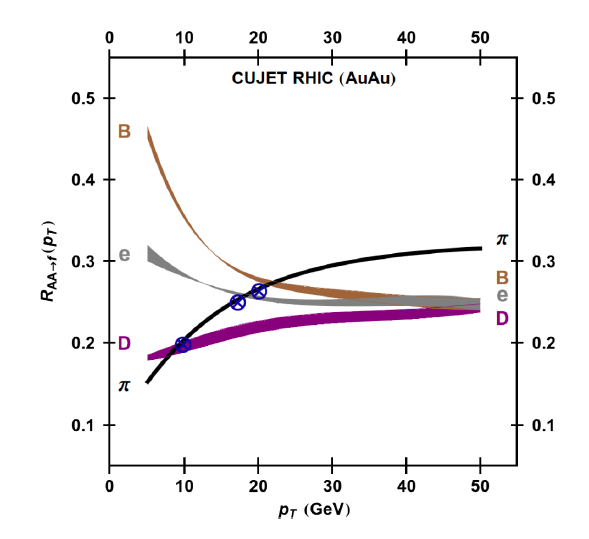
\includegraphics[width=0.45\textwidth]{fig/raa_CUJE.png}
\caption{Jet flavor tomography level crossing pattern of nuclear modification factors at middle rapidity of $\pi$, D, B, e calculations for central Au + Au 200 GeV collisions.}
\label{fig:raa_CUJE} 
\end{figure}

\begin{figure}
\centering
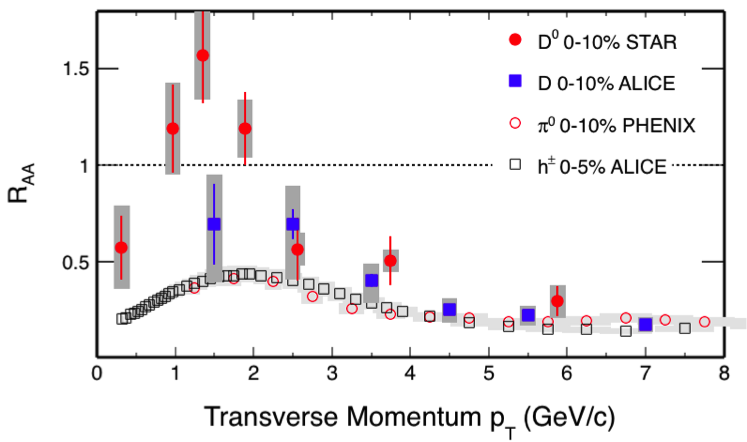
\includegraphics[width=0.5\textwidth]{fig/BeforeHFT.png}
\caption{(upper) $D^0$, $\pi$, $h^{\pm}$ $R_{AA}$ from different measurements. (bottom) $v_2$ of $D$ and $h^{\pm}$ from ALICE.}
\label{fig:BeforeHFT} 
\end{figure}

\section{\label{dataset}Datasets and Event Selection}

The dataset used in this analysis is P16id production of 2014 Au+Au 200 GeV data. This is the first year of physics running the new STAR HFT Detector. The analysis uses picoDst which is produced from MuDst.

The Minimum-Bias (MinBias) trigger is defined as a coincidence between the two VPDs, and an online collision vertex cut. Moreover, a pile-up protection at the trigger level was applied for the data taking. In this analysis, the MinBias trigger, denoted as ``vpdmb-5-p-nobsmd" and ``vpdmb-5-p-nobsmd-hlt", is used. The triggers used in this analysis are listed in Table~\ref{trigger}.

\begin{table}[htp]
\centering
\caption{Triggers ID used in this analysis from run14}
\label{trigger}
	\begin{center}
	\begin{tabular}{l|l}
%  \Xhline{1.6pt}
	Trigger ID	& description\\ \hline
	450050		& vpdmb-5-p-nobsmd-hlt\\ \hline
	450060		& vpdmb-5-p-nobsmd-hlt\\ \hline
	450005		& vpdmb-5-p-nobsmd\\ \hline
	450015		& vpdmb-5-p-nobsmd\\ \hline
	450025		& vpdmb-5-p-nobsmd\\ \hline
%  \Xhline{1.6pt}
	\end{tabular}
	\end{center}
\end{table}

Events used in this analysis are required to have a valid collision vertex $V_{z}$ (primary vertex) within 6 cm of the TPC center along $z$ direction (the beam direction) to ensure a uniform TPC acceptance and make sure the most tracks are within the PiXeL (PXL) detector coverage. The PXL detector is about 20 cm along the z direction, and the radius of the inner layer is about 2.8cm and outer layer is about 8 cm. Furthermore, the distance between the $V_{z}$ constructed by TPC and the vertex constructed by VPD ($V_{z}^{VPD}$, fast detector) is within 3 cm to reject the bad events. A radial length less than 2 cm for the vertex is required to reject the events from the beam hitting the beam pipe. After event selection, $\sim$875 million MinBias events are used for this analysis. Table~\ref{eventselection} lists the event selection criterion.

\begin{table}[htp]
\centering
\caption{Event selection in Au+Au collisions at 200 GeV for $D^0$.}
\label{eventselection}
\begin{tabular}{c}
\toprule[1.6pt]
Event Selection Criteria \\
\midrule[1.2pt]
\multirow{2}*{$!(|V_{x}|== 0 \ \&\& \ |V_{y}|== 0 \  \&\& \  |V_{z}|== 0) $ } \\
\\
\multirow{2}*{$|V_{z}|<$ 6 cm} \\
\\
\multirow{2}*{$|V_{r}|<$ 2 cm} \\
\\
\multirow{2}*{$|V_{z} - V_{z}^{VPD}|<$ 3 cm} \\ 
\\  
\bottomrule[1.6pt]
\end{tabular}
\end{table}

\subsection{Centrality Definition}

The centrality for Run14 200GeV Au+Au collisions MinBias sample is based on gRefMult. The gRefMult is defined as the number of global tracks with $|\eta|<0.5$, no less than 10 TPC hits, and Distance of Closest Approach (DCA) to primary vertex less than 3 cm with some correction according to $V_{z}$ and luminosity. The centrality definition according to the corrected gRefMult is listed in Table ~\ref{fig:centrality}. This is decided by comparing the measured gRefMult distribution with the Glauber model simulation. 

The basic procedure for centrality definition have three steps. First, need the quality assurance (QA) for the data set and remove those outlier runs. The second step would be correct the $V_{z}$ and luminosity dependence for the reference multiplicity (gRefmult). The last step would be compare our data with Glauber MC simulation and determine the centrality classification.

For the QA, several variables are used for the outlier selection, such as Refmult (primary track multiplicity), gRefmult (global track multiplicity), TofRefmult (tof track multiplicity) and etc. In the Fig.~\ref{fig:centrality_QA1} shows the $\langle$gRefmult$\rangle$ as a function of run index for the QA, and there are several outliers are identified. Those dashed lines are the 4$\times$RMS range, beyond those range, the runs are identified as bad run. And several iterations are did until all the runs are within these 4$\times$RMS range.


In the Fig.~\ref{fig:centrality_QA2} shows the $\langle$HFT $p_{T}$$\rangle$, which is the mean $p_{T}$ of HFT tracks, as a function of run index for the QA, and we can clearly see there is a deep before the run index $\sim$520 which corresponding to the run number 15107008. And also we saw the same structure in the Fig.~\ref{fig:centrality_QA3}, which shows the average of HFT matching Ratio in the $p_{T}$ range between 0.7 to 0.8 GeV/$c$ and Fig.~\ref{fig:centrality_QA4} shows this HFT matching ratio in the high $p_{T}$ range. So, basically those runs before day 107 were taken out for this analysis, since it will complicate our efficiency calculation.

This deep was identified later on with a lot of effort, it was due to the firmware issue. And more details can be found in the STAR documents below.

\url{https://drupal.star.bnl.gov/STAR/system/files/STAR_PXL_Firmware_Issue_Solved_Final_Report_Oct3_v2.pdf}

\begin{figure}[htbp]
\begin{minipage}[htbp]{0.52\linewidth}
\centering
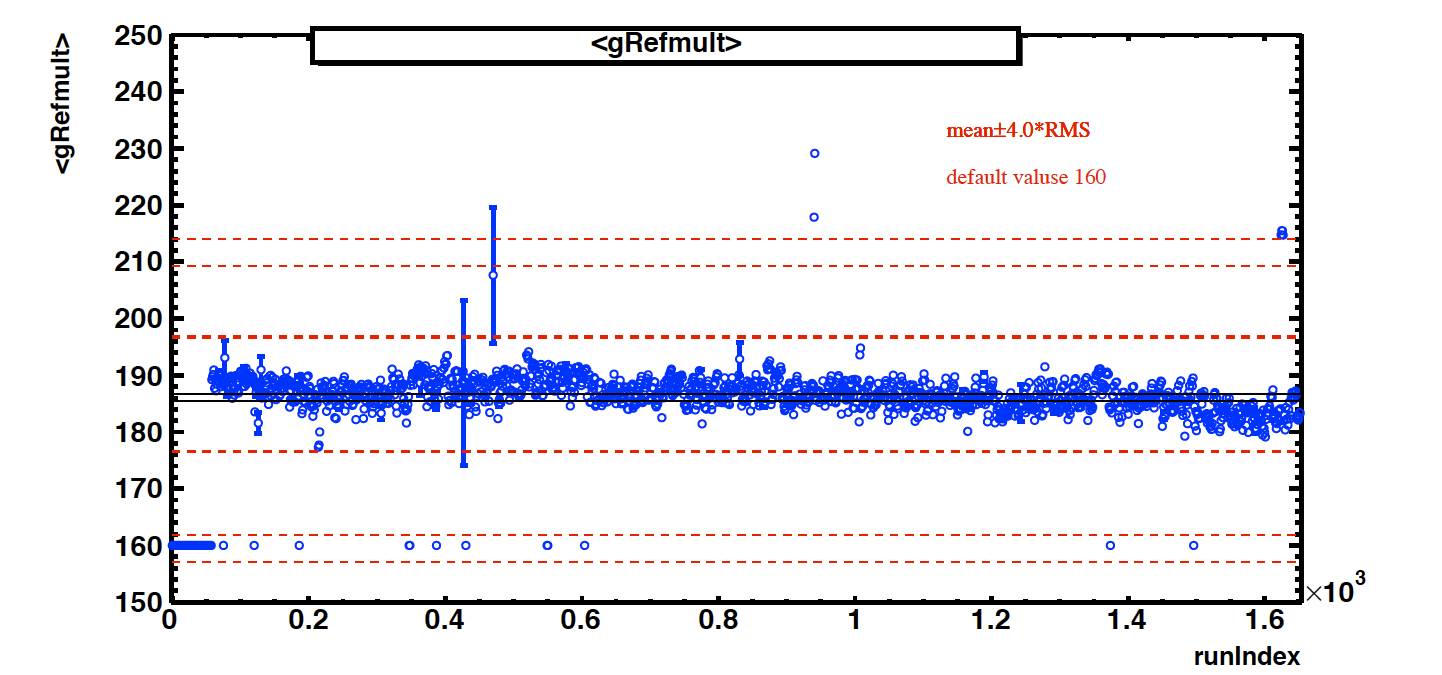
\includegraphics[width=1.0\textwidth]{fig/centrality_grefmult.png}
\caption{The mean value of gRefmult ($\langle$gRefmult$\rangle$) as a function of run index from QA.\label{fig:centrality_QA1}}
\end{minipage}
\hfill
\begin{minipage}[htbp]{0.52\linewidth}
\centering
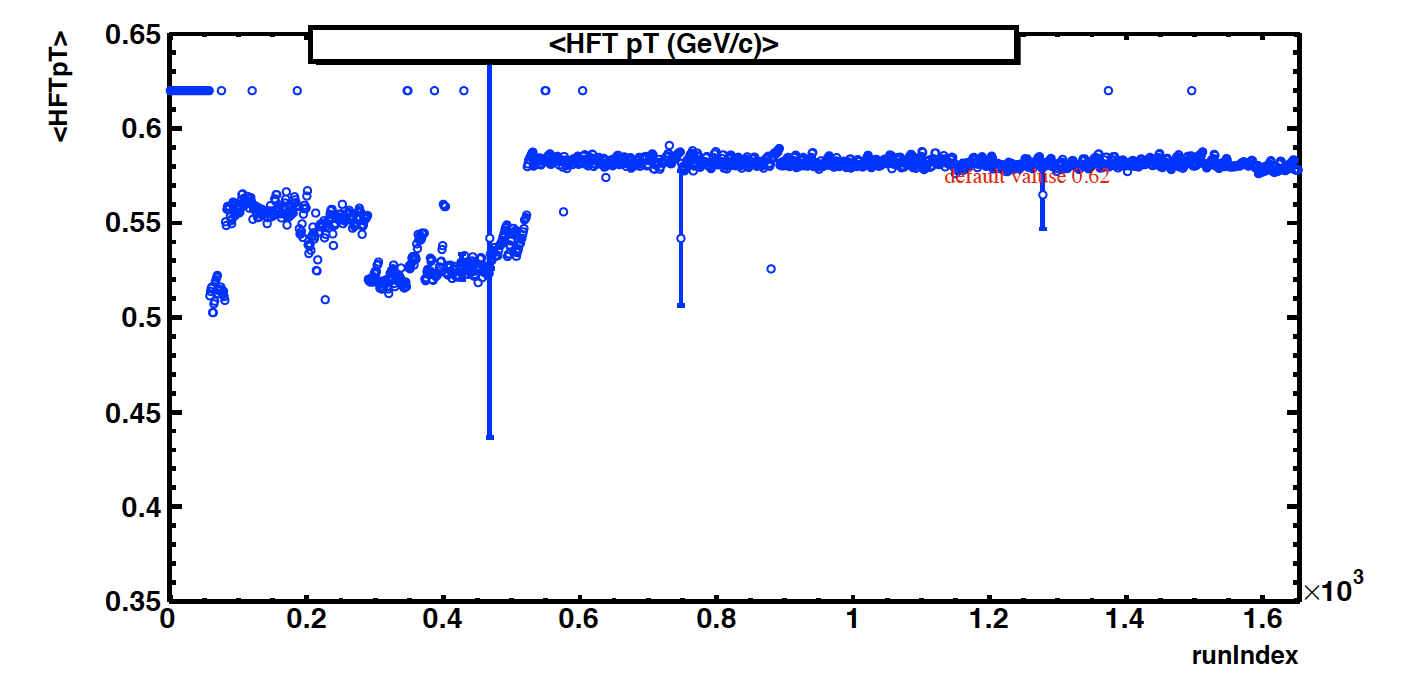
\includegraphics[width=1.0\textwidth]{fig/centrality_HFTpt.png} 
\caption{The mean value of $p_{T}$ for HFT matched track ($\langle$HFT $p_{T}$$\rangle$) as a function of index.\label{fig:centrality_QA2}}
\end{minipage}
\end{figure}


\begin{figure}[htbp]
\begin{minipage}[htbp]{0.52\linewidth}
\centering
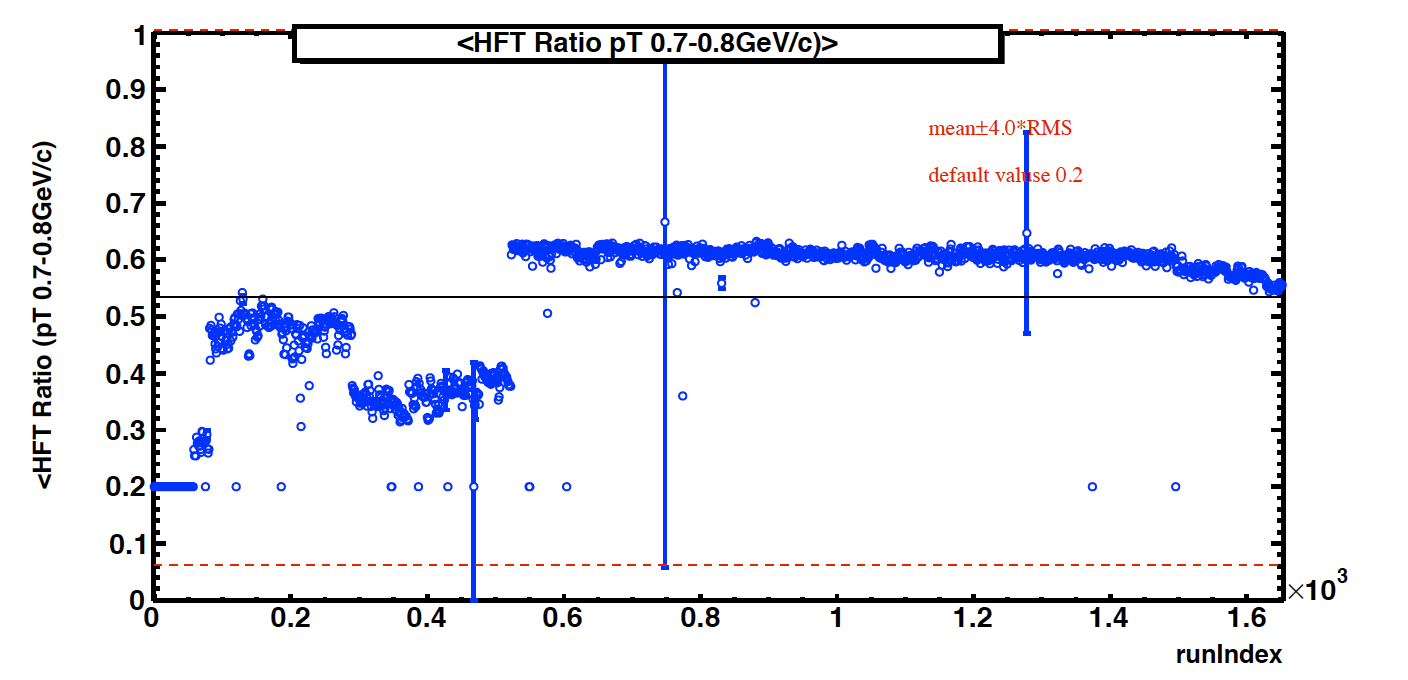
\includegraphics[width=1.0\textwidth]{fig/centrality_HFTratio.png}
\caption{The mean value of HFT matching ratio ($\langle$HFT $p_{T}$$\rangle$) as a function of run index at the transverse momentum range 0.7 < $p_{T}$ < 0.8 GeV/$c$.\label{fig:centrality_QA3}}
\end{minipage}
\hfill
\begin{minipage}[htbp]{0.52\linewidth}
\centering
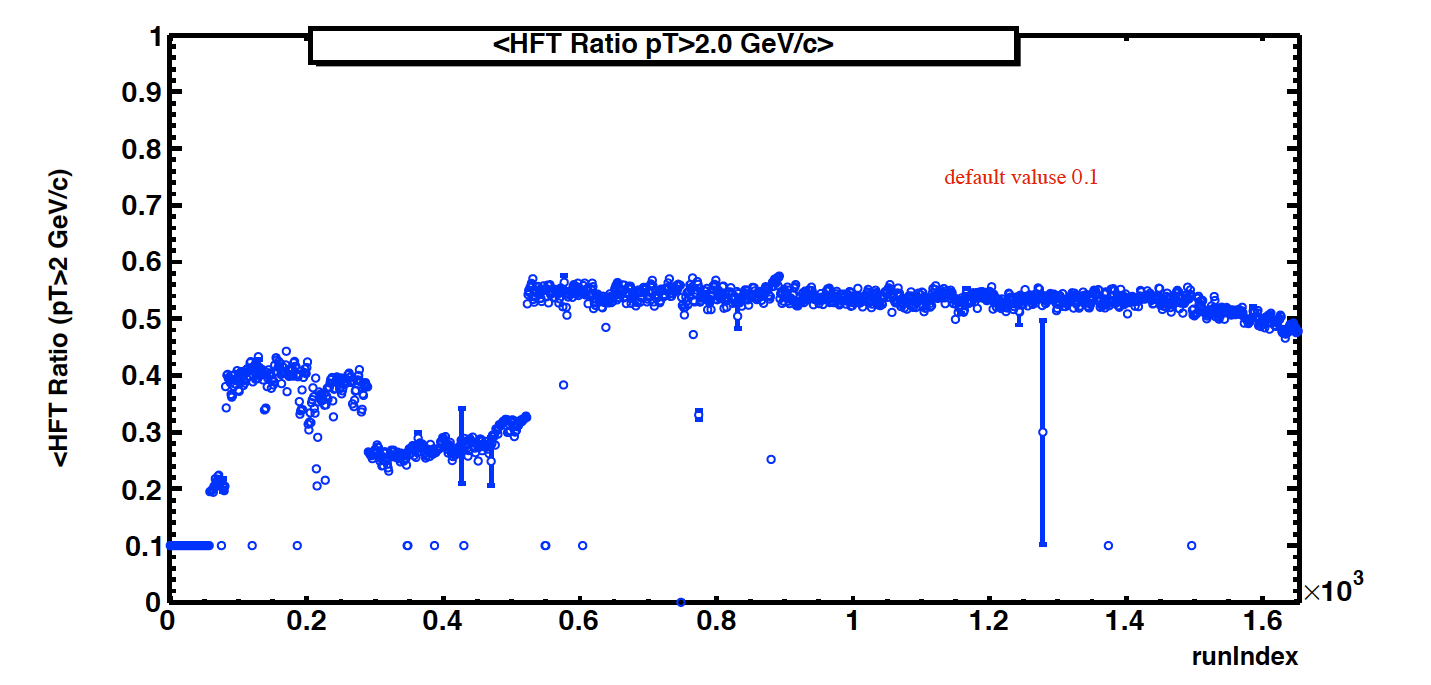
\includegraphics[width=1.0\textwidth]{fig/centrality_HFTratio2.png} 
\caption{The mean value of HFT matching ratio ($\langle$HFT $p_{T}$$\rangle$) as a function of run index at the transverse momenaum range $p_{T}$ > 2.0 GeV/$c$.\label{fig:centrality_QA4}}
\end{minipage}
\end{figure}

Fig.~\ref{fig:MB5_vz} and Fig.~\ref{fig:MB30_vz} show the normalized gRefmult distribution for several different $V_{z}$ range from -6 cm to 6 cm. The shape are quite different for VpdMB5 trigger in Fig.~\ref{fig:MB5_vz} while the Fig.~\ref{fig:MB30_vz} shows the same plots for VpdMB30 trigger ($V_z$ within range from -30 cm to 30 cm). This difference was explained by that the online Vpd vertex cut have a negative offset and the Vpd resolution has centrality dependence. As for the most central collisions, the resolution will be better than the most peripheral collisions. That is the reason we saw more events in the negative $V_{z}$ range and more central events for VpdMB5 trigger compared to VpdMB30 trigger.

\begin{figure}[htbp]
\begin{minipage}[htbp]{0.52\linewidth}
\centering
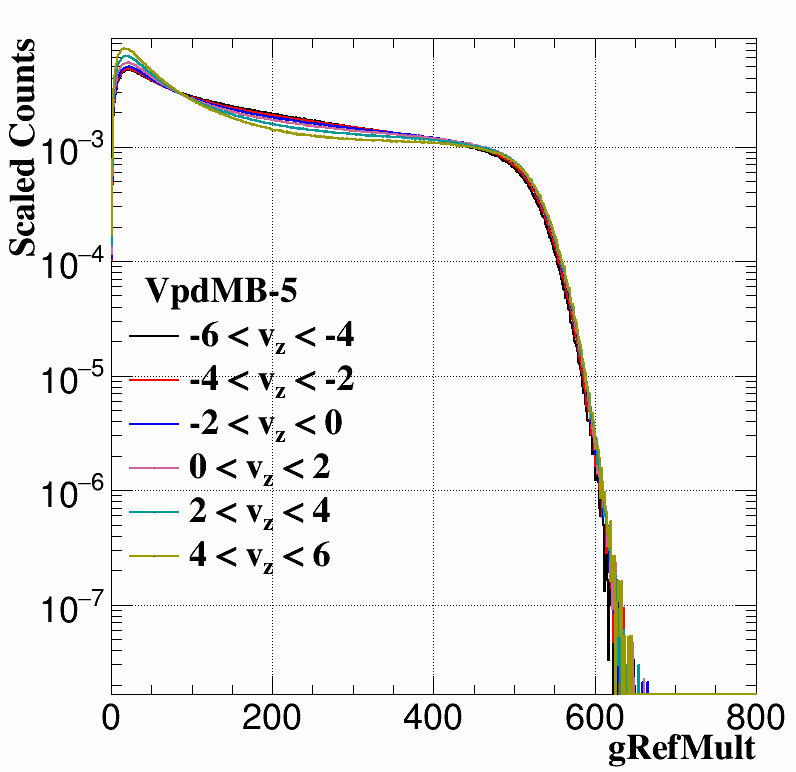
\includegraphics[width=0.75\textwidth]{fig/MB5_gref.png}
\caption{Normalized gRefmult distribution for VpdMB5 trigger along different $V_{z}$ range\label{fig:MB5_vz}}
\end{minipage}
\hfill
\begin{minipage}[htbp]{0.52\linewidth}
\centering
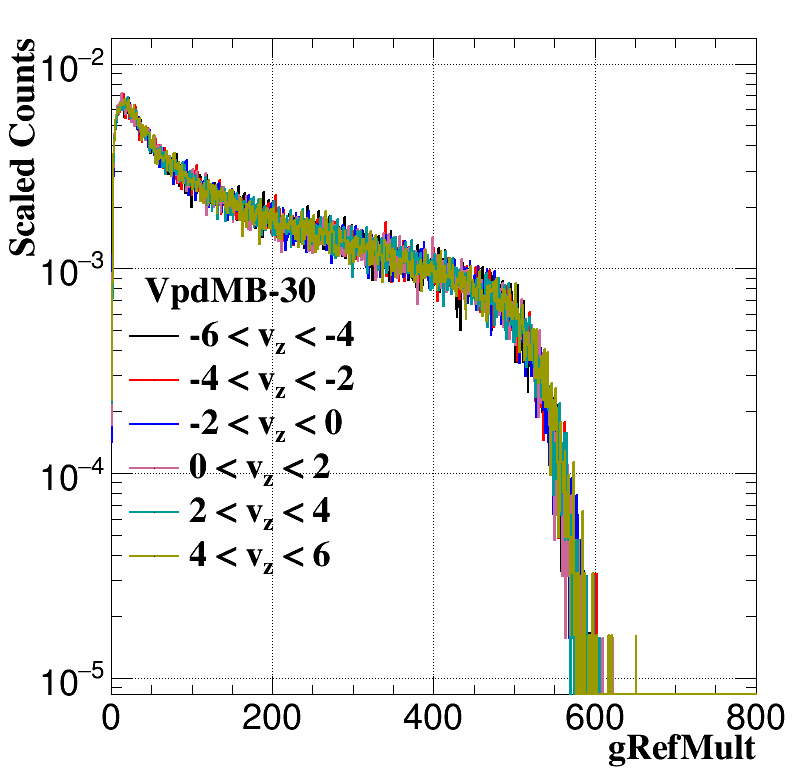
\includegraphics[width=0.75\textwidth]{fig/MB30_gref.png} 
\caption{Normalized gRefmult distribution for VpdMB30 trigger along different $V_{z}$ range\label{fig:MB30_vz}}
\end{minipage}
\end{figure}

As the gRefmult have the luminosity dependence (related to the TPC tracking efficiency have luminosity dependence), we need to take out this effect by doing ZdcX (Zdc coincidence rate) correction. Fig.~\ref{fig:MB5_zdc1} shows the mean value of gRefmult (<gRefmult>) distribution as a function of ZdcX. There was a clear slope for this distribution as shown by the fitting parameters. Here the fitting function is Eq.~\ref{funzdc},
\begin{equation}
f_{ZdcX} = p0 + p1*ZdcX
\label{funzdc}
\end{equation}
The goal of this correction is try to flatten this ZdcX dependence to take out of the luminosity effect. So here the correction factor was shown by  Eq.~\ref{funzdc2}.
\begin{equation}
f_{ZdcX} = \frac{1}{1 + p1/p0*ZdcX}
\label{funzdc2}
\end{equation}
After the ZdcX correction, this <gRefmult> is flat as shown by Fig.~\ref{fig:MB5_zdc2}.

For the $V_{z}$ dependence correction, we extract the high end point (h) from the fitting of gRefmult tail by the function of Eq.~\ref{funerf}.
\begin{equation}
f_{x} = A * TMath::Erf(-\sigma*(x-h)) + A
\label{funerf}
\end{equation}

\begin{figure}[htbp]
\begin{minipage}[htbp]{0.52\linewidth}
\centering
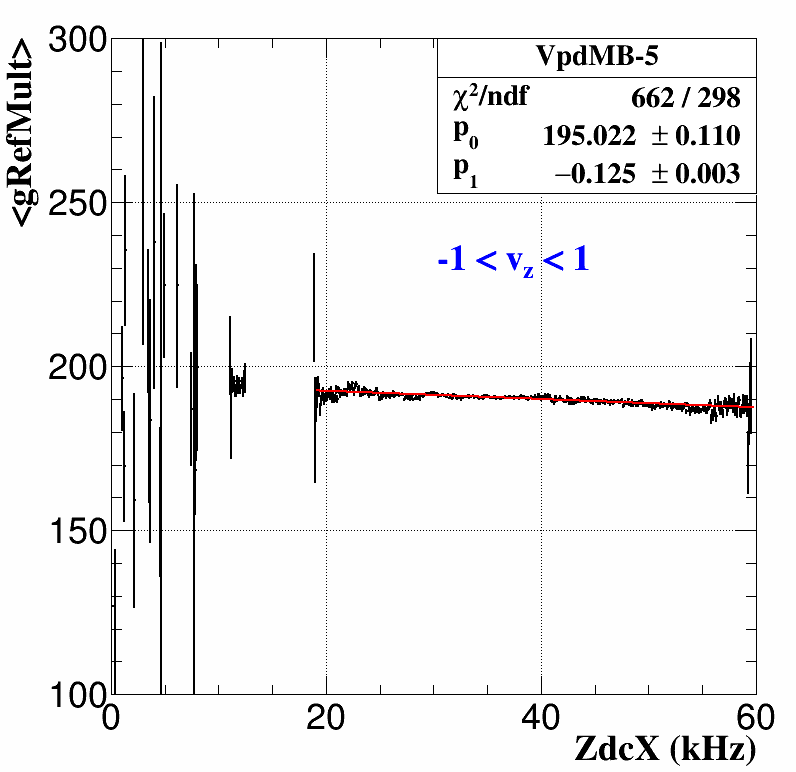
\includegraphics[width=0.75\textwidth]{fig/MB5_ZDCcor1.png}
\caption{<gRefmult> as function of ZdcX before correction.\label{fig:MB5_zdc1}}
\end{minipage}
\hfill
\begin{minipage}[htbp]{0.52\linewidth}
\centering
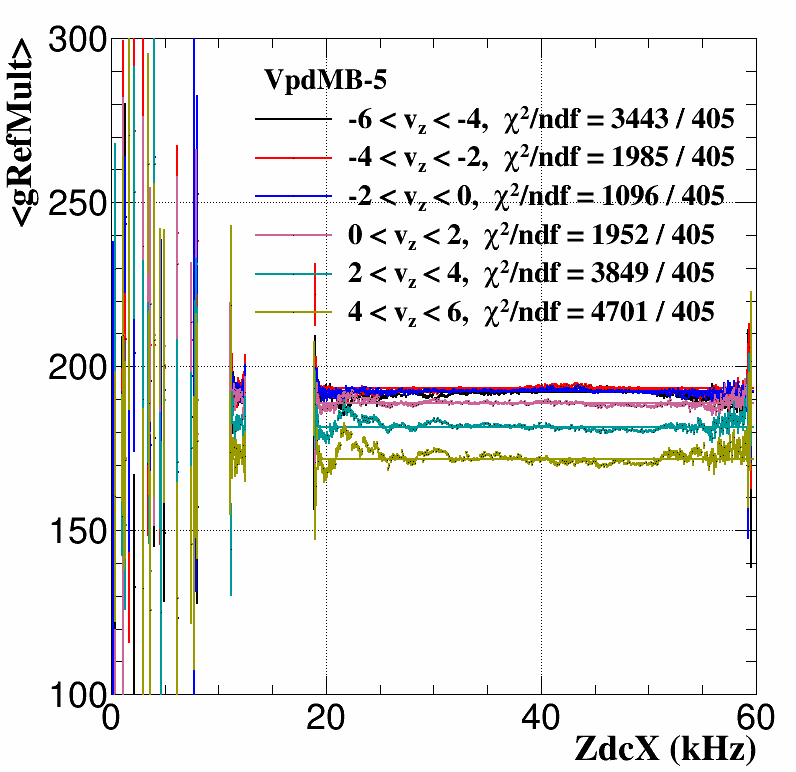
\includegraphics[width=0.75\textwidth]{fig/MB5_ZDCcor2.png} 
\caption{<gRefmult> as function of ZdcX after correction.\label{fig:MB5_zdc2}}
\end{minipage}
\end{figure}

Fig.~\ref{fig:MB5_vz1} shows an example of the fitting of gRefmult tail in the $V_{z}$ range from 1 cm to 2 cm. The fitting parameters were shown on the plot.

\begin{figure}[htbp]
\centering
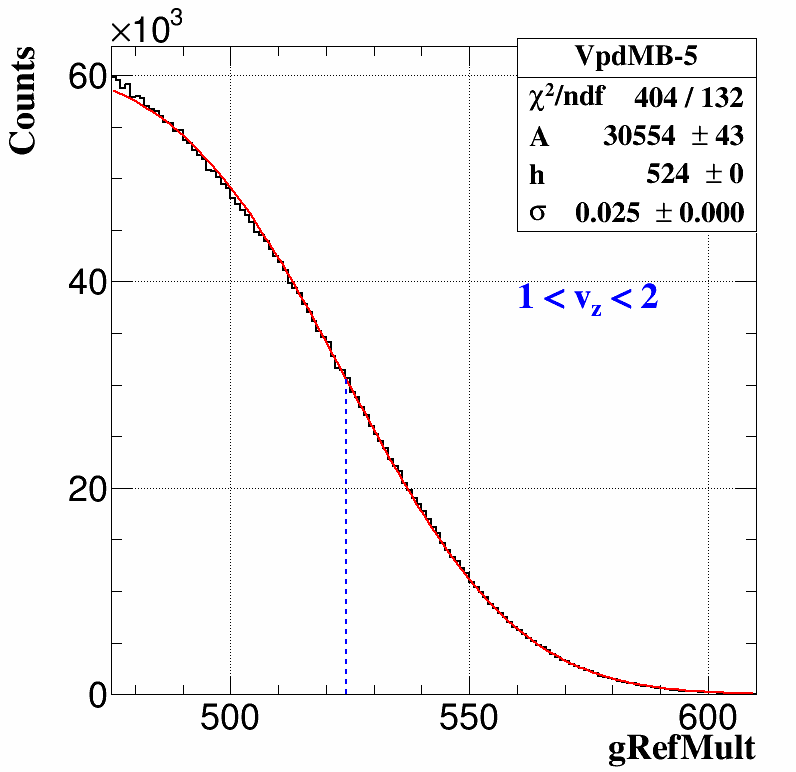
\includegraphics[keepaspectratio,width=0.5\textwidth]{fig/MB5_Vzcor1.png}
\caption{Fitting gRefmult tail distribution in the range of 1<$V_{z}$<2 cm by Eq.~\ref{funerf}.}
 \label{fig:MB5_vz1}
\end{figure}

With all the high end point value extracted along $V_{z}$ direction, this $V_{z}$ dependence was shown on Fig.~\ref{fig:MB5_vz2}. The similar method as ZdcX correction, we need to flatten this $V_{z}$ dependence, then the data point was fitted by 5th order polynomial function Eq.~\ref{funvz}, and then the correction factor was shown by Eq.~\ref{funvz2}
After the $V_{z}$ correction, this high end point is flat as shown by Fig.~\ref{fig:MB5_vz3}.

\begin{equation}
  f_{V_{z}} = p0 + p1*x + p2*x^2 + p3*x^3 + p4*x^4 + p5*x^5
\label{funvz}
\end{equation}

\begin{equation}
  f_{V_{z}} = \frac{p0}{p0 + p1*x + p2*x^2 + p3*x^3 + p4*x^4 + p5*x^5}
\label{funvz2}
\end{equation}


\begin{figure}[htbp]
\begin{minipage}[htbp]{0.52\linewidth}
\centering
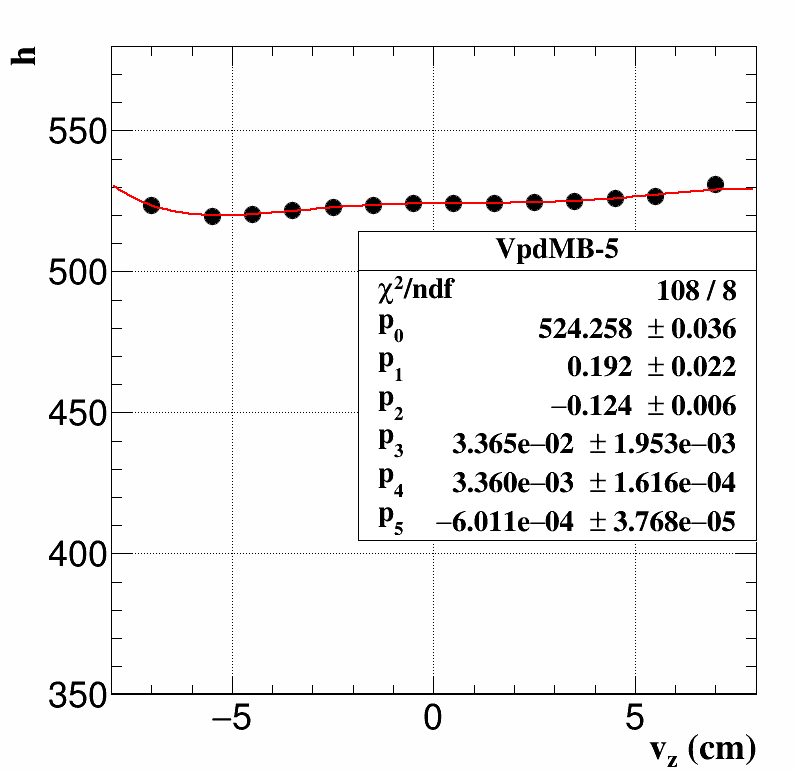
\includegraphics[width=0.75\textwidth]{fig/MB5_Vzcor2.png}
\caption{High end point as function of $V_{z}$ after correction.\label{fig:MB5_vz2}}
\end{minipage}
\hfill
\begin{minipage}[htbp]{0.52\linewidth}
\centering
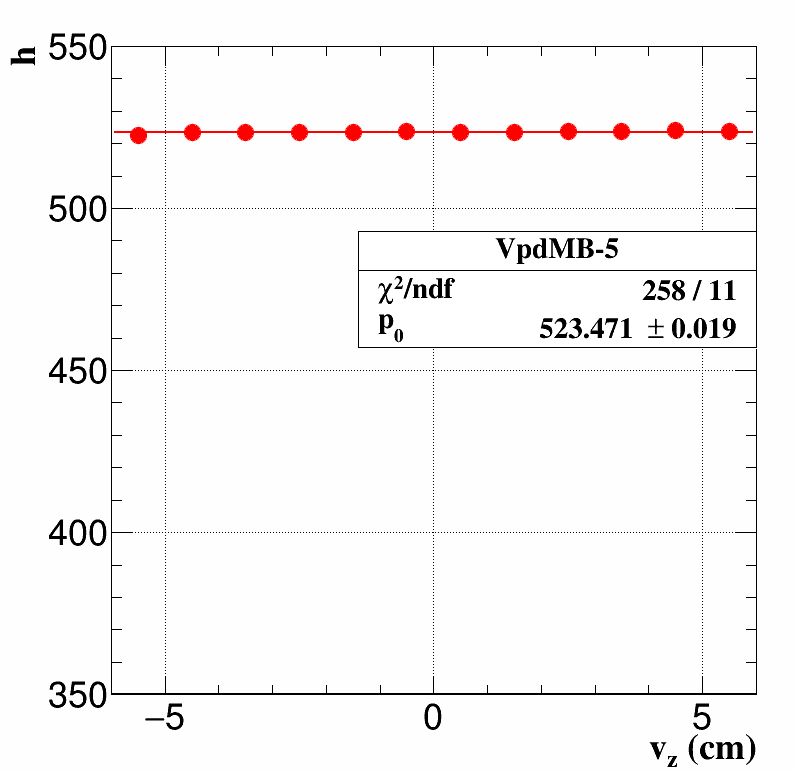
\includegraphics[width=0.75\textwidth]{fig/MB5_Vzcor3.png} 
\caption{High end point  as function of $V_{z}$ after correction.\label{fig:MB5_vz3}}
\end{minipage}
\end{figure}

As shown from Fig.~\ref{fig:MB5_vz} and Fig.~\ref{fig:MB30_vz}, the clear $V_{z}$ dependence need to avoid for VpdMB5 trigger. So, the centrality definition for VpdMB5 trigger was normalized to VpdMB30. After the ZdcX correction and $V_{z}$ correction, we directly take it as an additional correction factor for VpdMB5. These correction factor was show in Fig.~\ref{fig:MB5_vzscale}. After this additional correction, the distributions from VpdMB5 and VpdMB30 are same.

\begin{figure}[htbp]
\centering
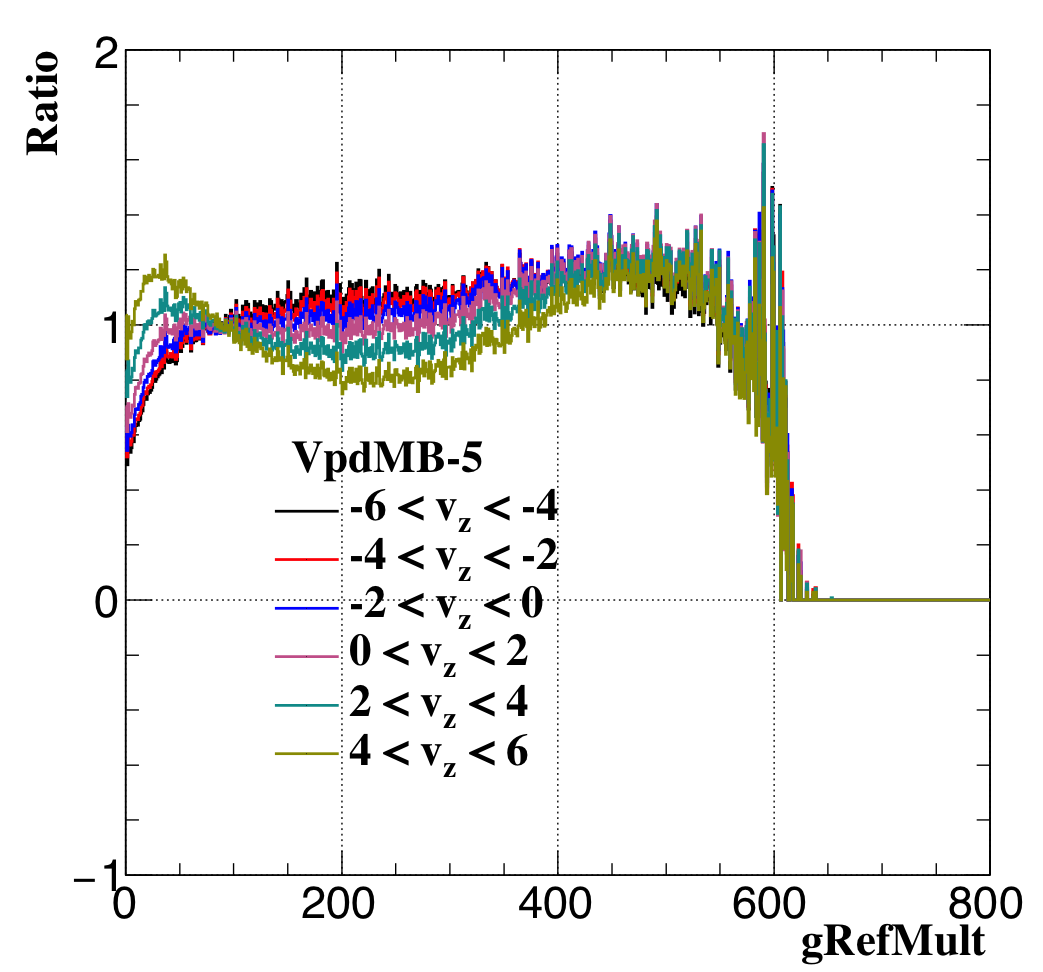
\includegraphics[keepaspectratio,width=0.5\textwidth]{fig/MB5_VzScale.png}
\caption{The double ratio of normalized gRefmult distribution from VpdMB5 over VpdMB30, this additional correction factor was try to normalized VpdMB5 to VpdMB30 trigger.}
 \label{fig:MB5_vzscale}
\end{figure}

The Vpd MinBias trigger has a trigger efficiency that are lower for periheral events. Fig.~\ref{fig:McData} shows the gRefmult after $V_{z}$ and ZdcX correction from data comparison with Glauber MC simulation. In the high end part the agreement was well, but in the low end part, due to this trigger ineffciency, there is clearly discrepancy between data and simulation. To do the measurement without centrality bias, a weight proportional to inverse trigger efficiency is applied. The weight as a function of corrected gRefMult is shown in Fig.~\ref{fig:vpdEffWeight}.

\begin{figure}[htbp]
\begin{minipage}[htbp]{0.52\linewidth}
\centering
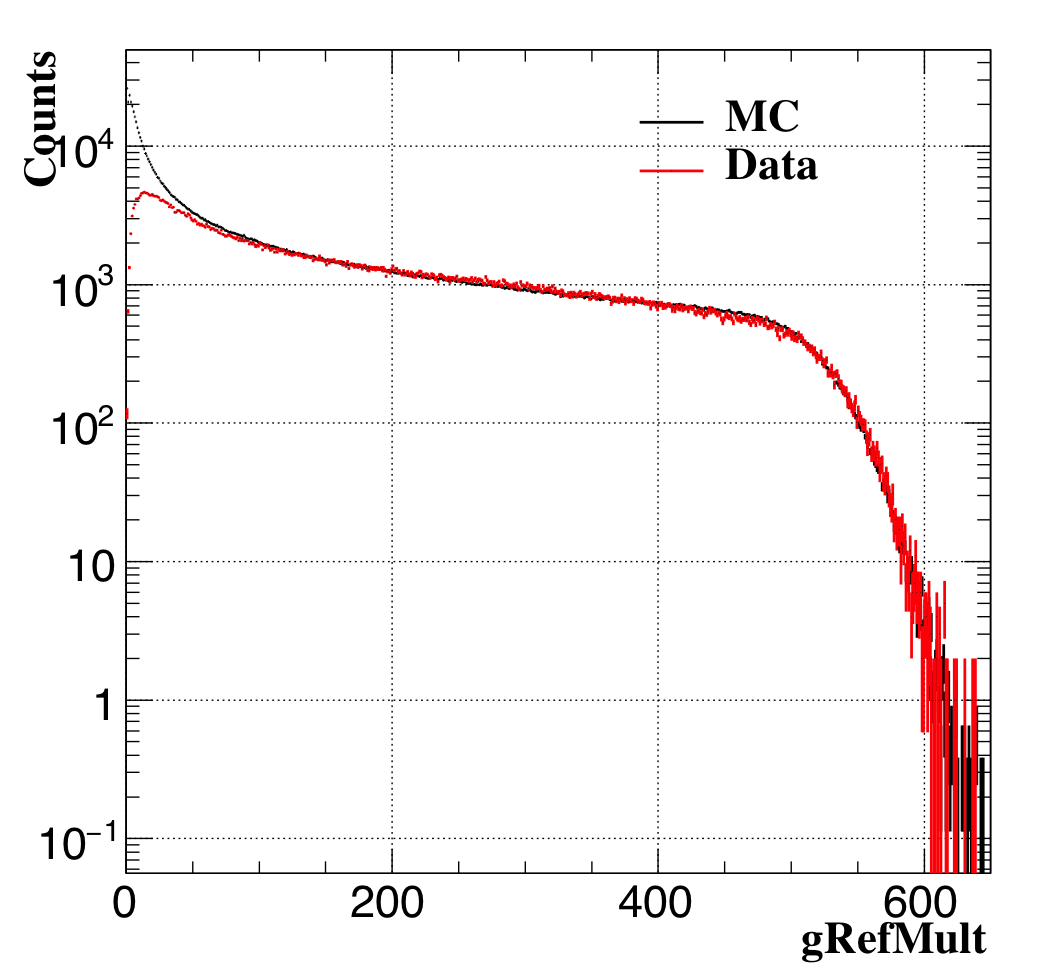
\includegraphics[width=0.75\textwidth]{fig/MB30_Mc_compare.png}
\caption{The comparison of corrected gRefMult between Data and Glauber MC. The red line is data and the black line is from Glauber MC.\label{fig:McData}}
\end{minipage}
\hfill
\begin{minipage}[htbp]{0.52\linewidth}
\centering
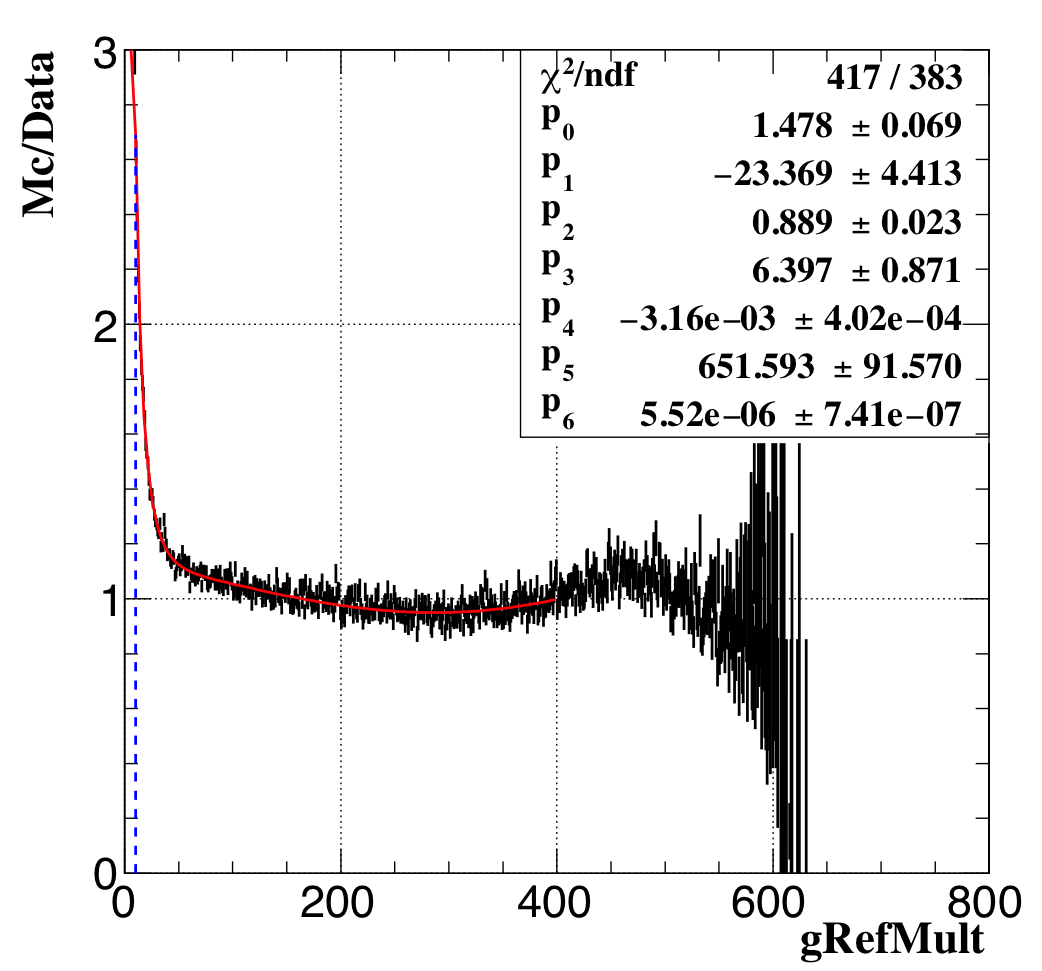
\includegraphics[width=0.75\textwidth]{fig/MB30_Mc_reweight.png} 
\caption{MC/data gRefmult distribution for Vpd MinBias trigger efficiency correction. The red line fit function is the correction reweight function.\label{fig:vpdEffWeight}}
\end{minipage}
\end{figure}

\begin{figure}[htbp]
\centering
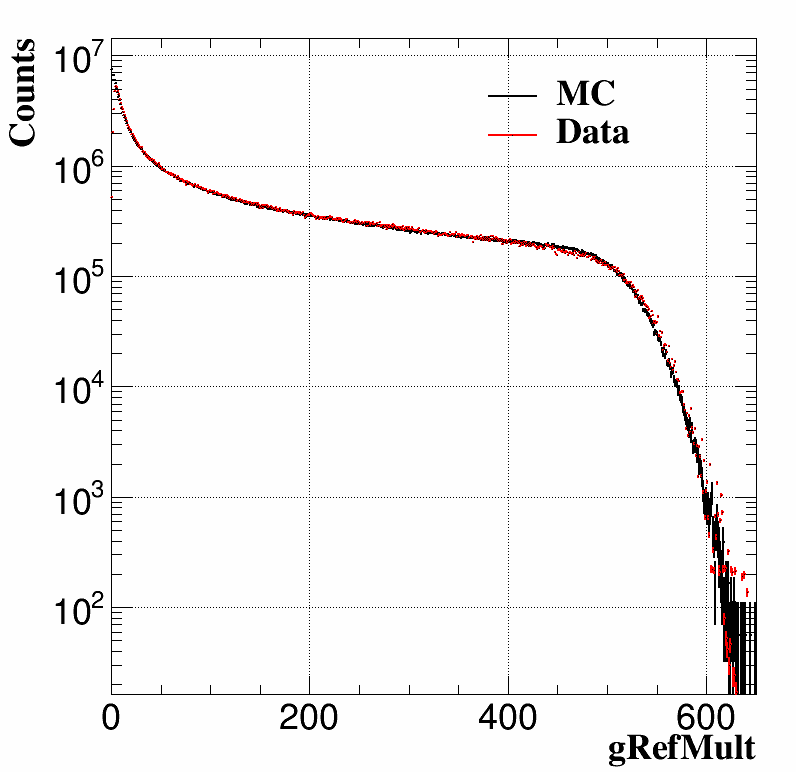
\includegraphics[keepaspectratio,width=0.5\textwidth]{fig/MB5_AfterALLMCData.png}
\caption{The comparison of corrected gRefMult (after all corrections and reweight) between Data and Glauber MC. The red line is data and the black line is from Glauber MC.\label{fig:MB5_afterAll}}
\end{figure}

After all these corrections including $V_{z}$, ZdcX, Vpd trigger inefficiency, and Vpd resolution for different centralities as discussed before. Final step, the data was compared to Glauber MC simulation as shown in Fig.~\ref{fig:MB5_afterAll}. And then the determined centrality classification can be found at Table ~\ref{centrality}.

\begin{table}[htp]
	\begin{center}
	\begin{tabular}{l|l|l|l}
  \toprule[1.6pt]
  \hline
  centrality & gRefMult & {$\langle$$N_{coll}$$\rangle$} & {$\langle$$N_{part}$$\rangle$} \\ \hline
  75-80$\%$ &	10-15	& 10.48 &	11.82 \\ \hline
	70-75$\%$ &	15-21	&	16.11 &	16.68 \\ \hline
	65-70$\%$ &	21-30	&	24.59 &	23.25 \\ \hline
	60-65$\%$ &	30-41	&	36.13 &	31.15 \\ \hline
	55-60$\%$ &	41-56	&	52.77 &	41.27 \\ \hline
	50-55$\%$ &	56-73	&	75.36 &	53.46 \\ \hline
  45-50$\%$ &	73-94	&	105.25 & 67.93 \\ \hline
  40-45$\%$ &	94-119 & 143.54 &	84.71 \\ \hline
  35-40$\%$ &	119-148	& 191.83 & 103.99 \\ \hline
	30-35$\%$ &	148-182	& 253.13 & 126.52 \\ \hline
	25-30$\%$ &	182-221	& 328.99 & 152.31 \\ \hline
	20-25$\%$ &	221-266	& 422.49 & 181.93 \\ \hline
	15-20$\%$ &	266-317	& 537.52 & 215.98 \\ \hline
	10-15$\%$ &	317-376	& 677.99 & 254.90 \\ \hline
	5-10 $\%$ &	376-443	& 852.75 & 299.95 \\ \hline
  0-5	 $\%$	& $>$443	& 1066.50	& 348.74 \\ \hline
  \hline
  \bottomrule[1.6pt]
	\end{tabular}
	\caption{Centrality defintion based on gRefMult}
	\label{centrality}
	\end{center}
\end{table}

\section{$D^0$ Reconstruction}

$D^{0}$ and $\bar{D^{0}}$ are reconstructed through the typically hadronic channel $K^{\mp}\pi^{\pm}$ using the topological method. In the following we will describe the daughter selection, the geometry cuts and how they are obtained through the TMVA tuning. We will show the $D^0$ signals for different $p_T$ bins. We will also discuss some related topics: the mixed event to reconstruct the combinatorial background, and the correlated background source shown as a `bump' at invariant mass lower than the $D^0$. 

\subsection{Daughter Selection}
\label{daughterSelection}
$D^0$ have a lifetime of $c\tau\sim123 \upmu$m. Thus the global tracks for daughter tracks are used in this analysis. The transverse momentum are required to $\geq$ 0.3 GeV/$c$ to ensure that the track can pass through the TPC and have less HFT miss matching, the number of hit points (nHits) along the track is $\geq$ 20 (of a maximum of 45) to ensure good momentum resolution.

The pion and kaon tracks are identified by combining Time Projection Chamber (TPC) and Time Of Flight detector (TOF). The TPC provides particle identification utilizing the energy loss information $dE/dx$, different particle species with the same momentum may have different $dE/dx$. In additional, different particle species with the same momentum have different velocities, thus the TOF can be used to identify different particle species in the $dE/dx$ crossover regions by precise velocity information ($1/\beta$ = $ct/l$). The normalized $dE/dx$, $n\sigma_x$ (x = $\pi$, K, p, e etc.), defined in Eq.~\ref{nsigma}, instead of $dE/dx$ is used in this analysis. Where $\langle{dE/dx}\rangle_{measured}$ and $\langle{dE/dx}\rangle_{x}$ represent measured and theoretical $dE/dx$, and $R$ is the STAR TPC $dE/dx$ resolution (typically $\sim$8\%). The $n\sigma_x$ should be close to a standard Gaussian distribution for each corresponding particle species (mean $=$ 0, $\sigma = $ 1).
\begin{equation}
  n\sigma_x = \frac{1}{R}log\frac{\langle{dE/dx}\rangle_{measured}}{\langle{dE/dx}\rangle_{x}}
\label{nsigma}
\end{equation}

Fig.~\ref{fig:tpcPID} shows the TPC energy loss dE/dx information versus momentum achieved from Run14 Au+Au 200GeV, there are several clear bands for different particle species such as $\pi$, K, p and e. 

Fig.~\ref{fig:tofPID} shows the TOF 1/Beta information versus momentum achieved from Run14 Au+Au 200GeV, also there are several clear bands for different particle species such as $\pi$, K, p . 

\begin{figure}[htbp]
\centering
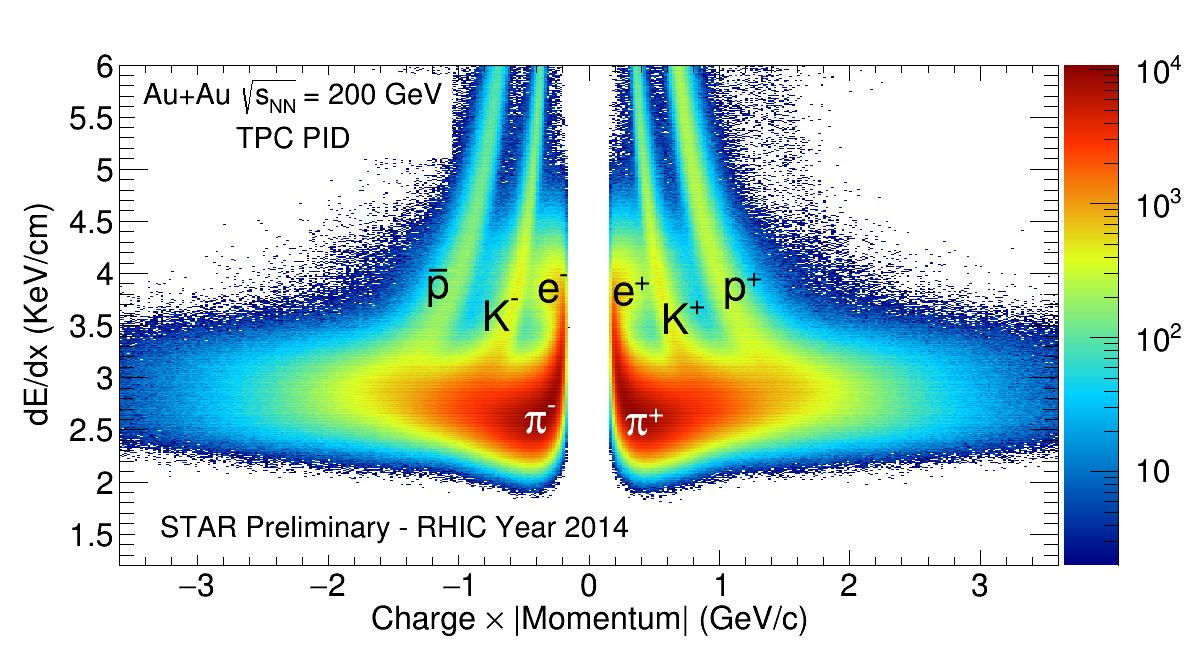
\includegraphics[keepaspectratio,width=0.8\textwidth]{fig/Run14_AuAu_dEdx_PR_copy.png}
\caption{TPC dE/dx versus charge$\times$momentum achieved from Run14 Au+Au 200GeV.}
 \label{fig:tpcPID}
\end{figure}

\begin{figure}[htbp]
\centering
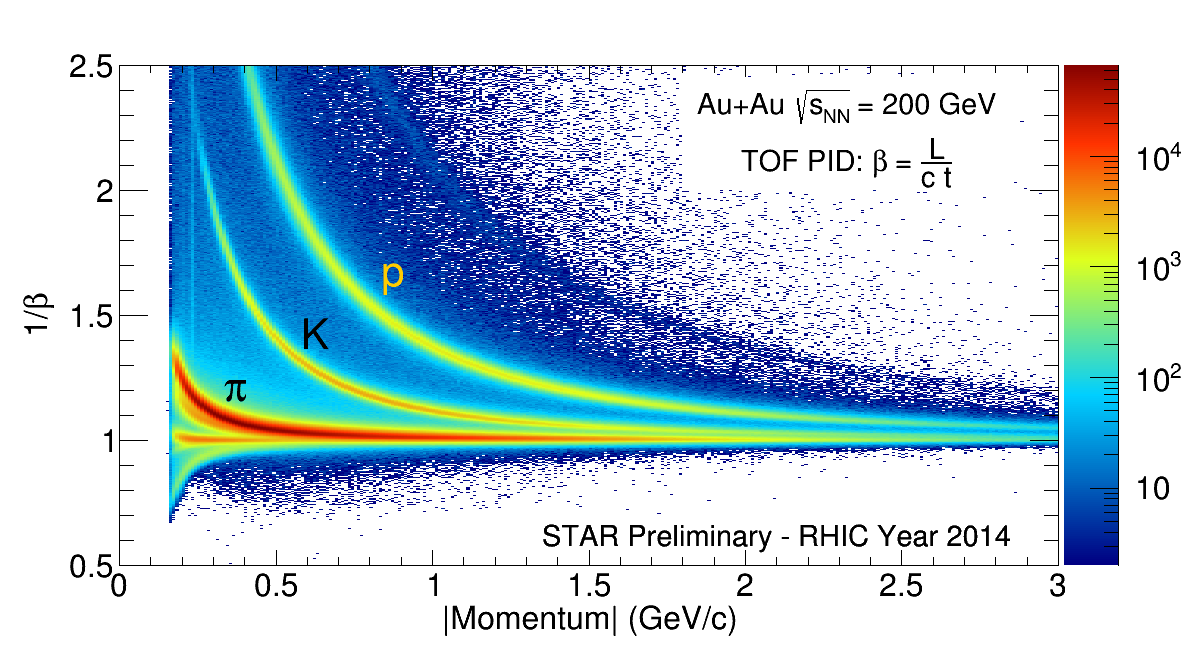
\includegraphics[keepaspectratio,width=0.8\textwidth]{fig/Run14_AuAu_tofBeta_PR.png}
\caption{TOF 1/Beta versus momentum achieved from Run14 Au+Au 200GeV.}
 \label{fig:tofPID}
\end{figure}

In summary, next list all the related track selections for $D^0$ daughters including track quality cut and particle identification cut.
\begin{itemize}
\item global tracks
\item $p_{T}$ > 0.3 GeV/$c$
\item $|\eta| < 1$
\item $nHitsFit \ge 20$, in TPC
\item at least one hit in every layer of PXL and IST
\end{itemize}

pion PID:
\begin{itemize}
  \item $|n\sigma_{\pi}| < 3.0 $, based on TPC dE/dx
  \item If TOF is avaliable (hybrid PID):  $|\frac{1}{\beta}-\frac{1}{\beta_{exp}}|<0.03$
\end{itemize}

kaon PID:
\begin{itemize}
  \item $|n\sigma_{K}| < 2.0 $, based on TPC dE/dx
  \item If TOF is avaliable (hybrid PID):  $|\frac{1}{\beta}-\frac{1}{\beta_{exp}}|<0.03$
\end{itemize}


\subsection{Topological Cut Optimization}

The secondary vertex is reconstructed with selected kaon and pion global tracks. In this analysis, the middle point on the Distance of the Closest Approach (DCA) between two daughter tracks is considered as the secondary decay vertex of the candidate $D^0$. As shown in Fig.~\ref{fig:D0cartoon}, 5 geometrical variables are chosen to select $D^0$ and reject combinatorial background, which is dominated by a pair of tracks directly from the primary vertex: decay length (the distance between the decay vertex and Primary Vertex PV), DCA between the 2 daughters, DCA between the reconstructed $D^0$ flying path and PV, DCA between the $\pi$ track and PV, and DCA between the $K$ track and PV. The cuts on these variables are optimized by the Toolkit for Multivariate Data Analysis (TMVA) package. They change according to the $D^0$ candidate $p_T$ in order to have the best significance in all the covered $p_T$ range. Additionally there is a $cos(\theta) > 0$ cut to make sure the decay vertex with respect to the primary vertex is roughly in the same direction as the momentum.

\begin{figure}[htbp]
\centering
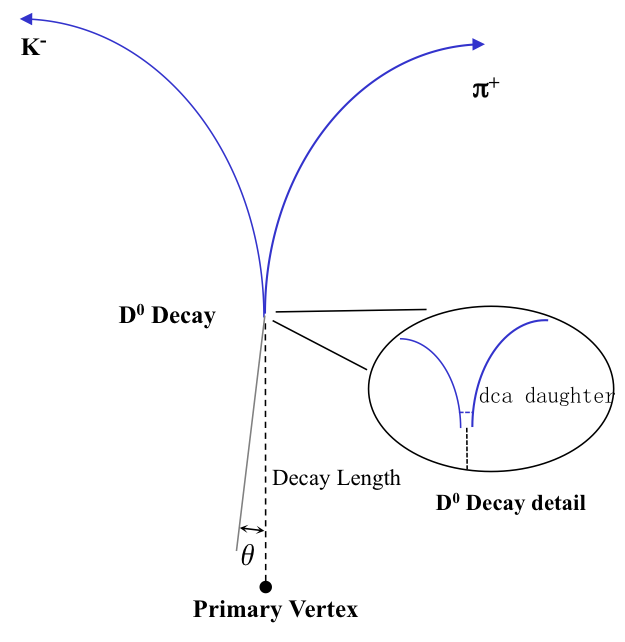
\includegraphics[keepaspectratio,width=0.6\textwidth]{fig/D0cartoon.png}
\caption{The topology of a $D^0$ decaying to a kaon and a pion.}
 \label{fig:D0cartoon}
\end{figure}

The TMVA need signal and background sample input for training. The signal sample is obtained from a toy fast-simulation and the background sample is from real data like sign pairs in $D^0$ mass window and unlike sign pairs in side bands range. 

Fig.~\ref{fig:variables} shows distributions of the 5 geometry variables for signal (blue) and background (red) plotted by the TMVA, for $p_T$ between 2 and 3 GeV/$c$.

\begin{figure}[htbp]
\centering
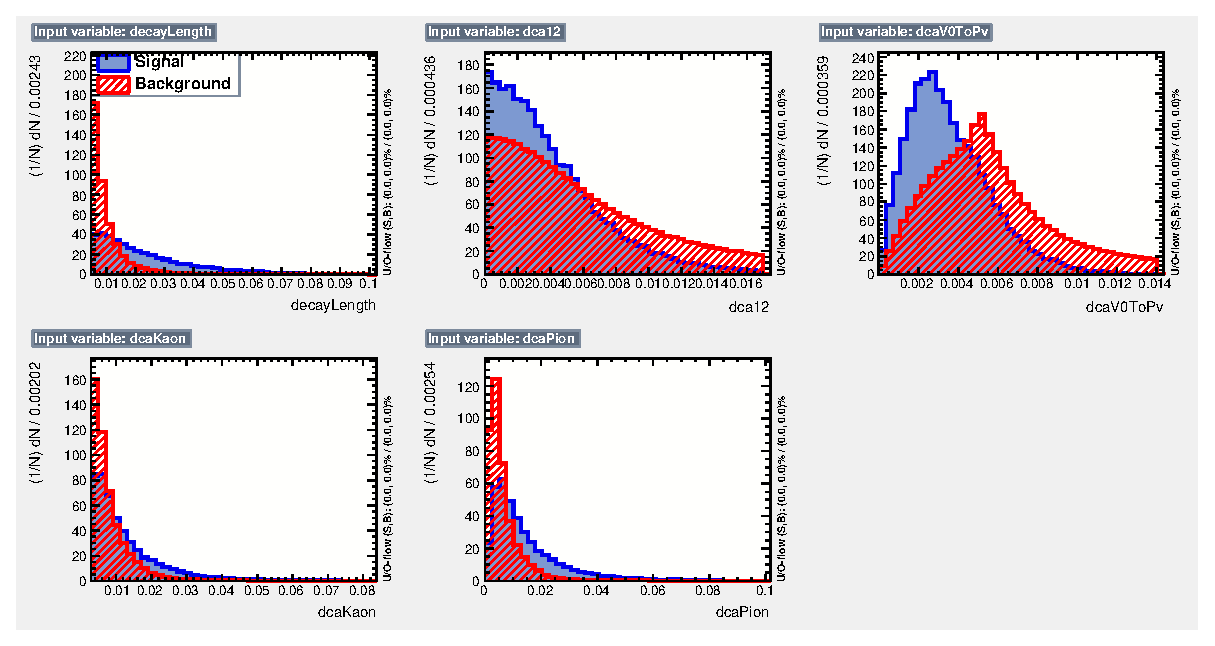
\includegraphics[keepaspectratio,width=1.0\textwidth]{fig/variables_id_c1.eps}
\caption{Distributions of the 5 geometry variables for signal (blue) and background (red).}
\label{fig:variables}
\end{figure}

The `cuts' option of TMVA is used to tune $D^0$ cuts. This option randomly sample different cut sets in the variable space, calculate signal and background efficiency for each cut set. Then one cut set with lowest background efficiency at certain signal efficiency. We can then pick the cut set with the best significance according to the signal and background yield corresponding to the whole data set. Fig.~\ref{fig:effPass4} shows the lowest background efficiency, significance and so on vs. signal efficiency for $p_T$ between 2 and 3 GeV/$c$. We can see that as cuts get tighter, signal and background efficiency both decrease, but background efficiency decreases much faster.

\begin{figure}[htbp]
\centering
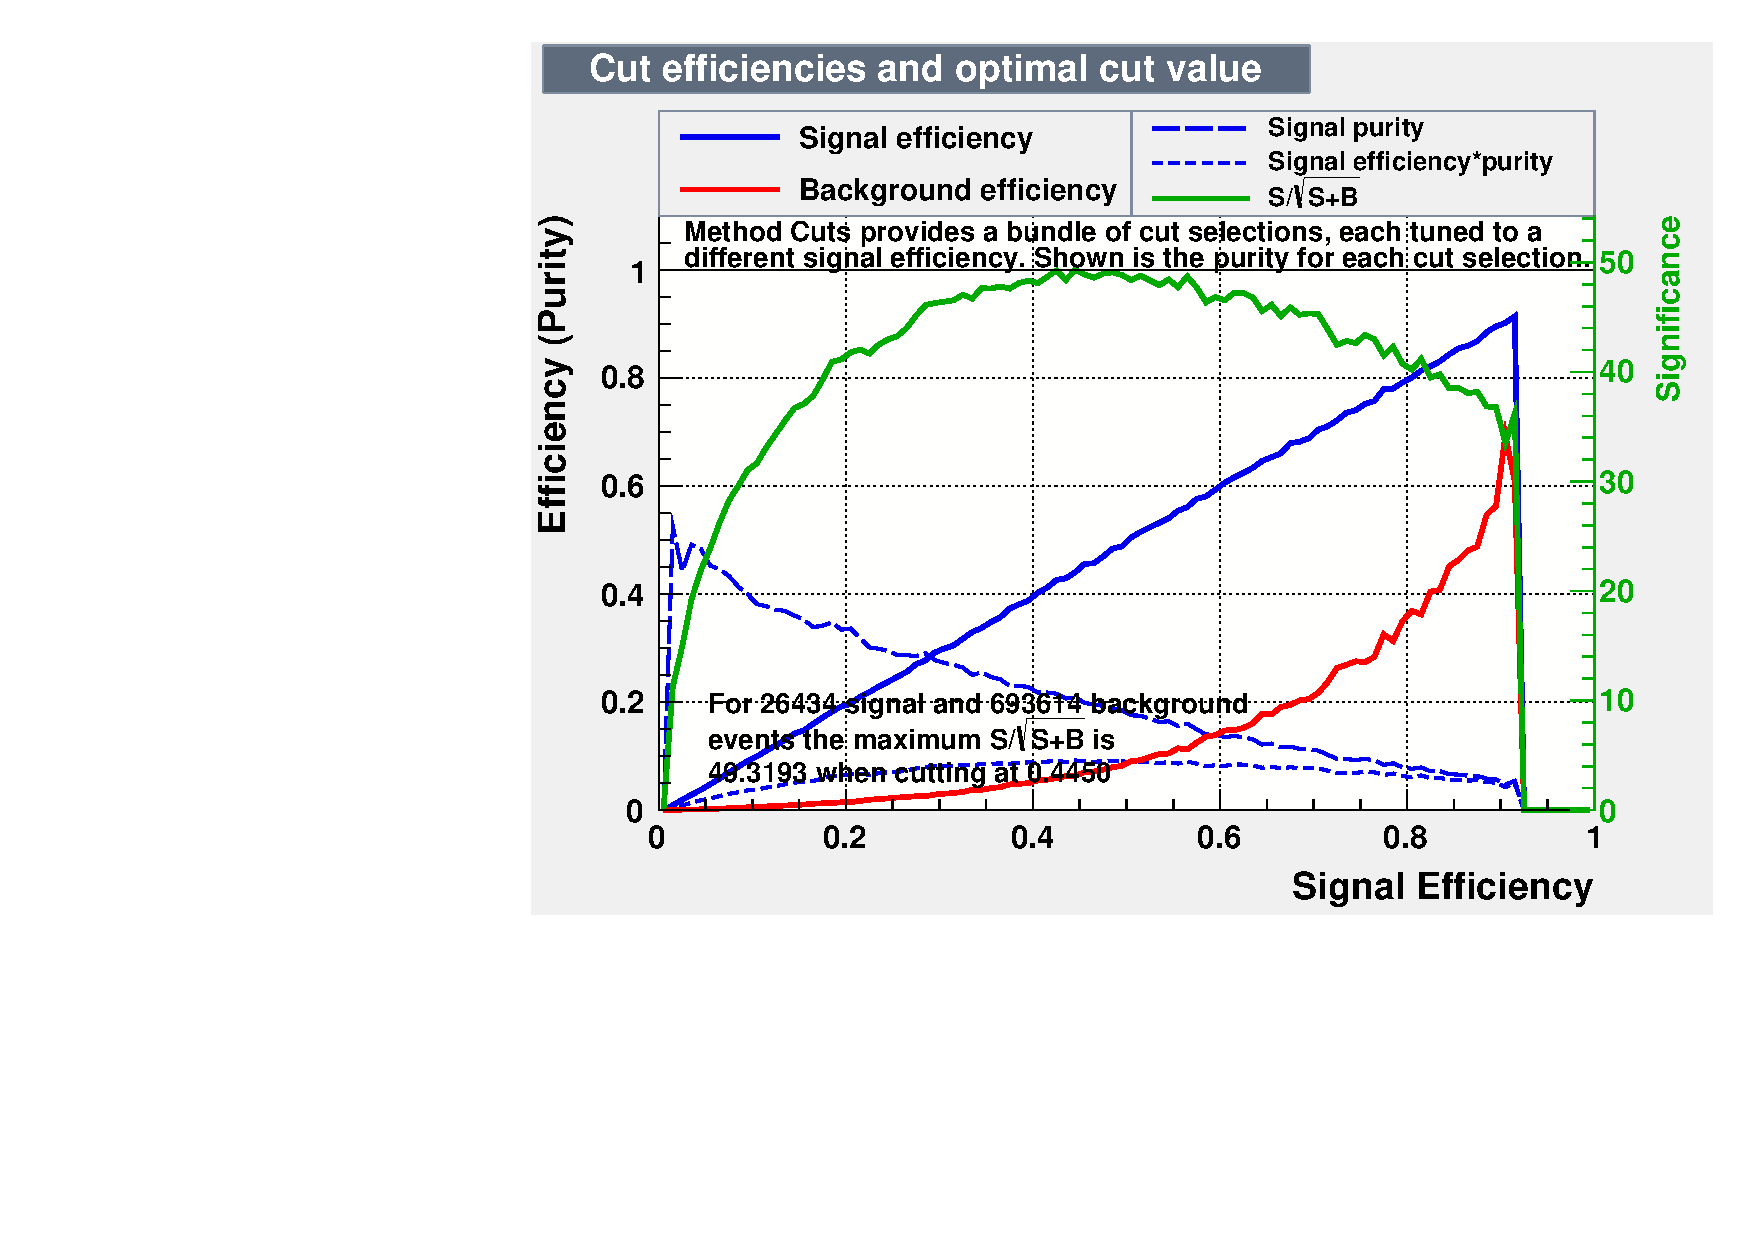
\includegraphics[keepaspectratio,width=0.5\textwidth,angle=0]{fig/effPass4.pdf}
\caption{Signal efficiency, lowest background efficiency, significance and so on vs. signal efficiency.}
\label{fig:effPass4}
\end{figure}

\begin{table}[htp]
  \centering
  \caption{Standard geometrical cuts for different $D^0$ $p_T$.}
  \label{geometryCuts}
  \begin{center}
    \begin{tabular}{l|l|l|l|l|l}
      % \Xhline{1.6pt}
      $D^0$ $p_T$ (GeV/$c$) & 0-1 & 1-2 & 2-3 & 3-5 & 5-10\\ \hline
      decay length (${\upmu}m$) $>$ & 145 & 181 & 212 & 247 & 259\\ \hline
      DCA between 2 daughters (${\upmu}m$) $<$ & 84 & 66 & 57 & 50 & 60\\ \hline
      DCA between $D^0$ and PV (${\upmu}m$) $<$ & 61 & 49 & 38 & 38 & 40\\ \hline
      DCA between $\pi$ and PV (${\upmu}m$) $>$ & 110 & 111 & 86 & 81 & 62\\ \hline
      DCA between $K$ and PV (${\upmu}m$) $>$ & 103 & 91 & 95 & 79 & 58\\ \hline
      % \Xhline{1.6pt}
    \end{tabular}
  \end{center}
\end{table}

\begin{table}[htp]
  \centering
  \caption{Tight geometrical cuts for different $D^0$ $p_T$.}
  \label{geometryCutsTight}
  \begin{center}
    \begin{tabular}{l|l|l|l|l|l}
      % \Xhline{1.6pt}
      $D^0$ $p_T$ (GeV/$c$) & 0-1 & 1-2 & 2-3 & 3-5 & 5-10\\ \hline
      decay length (${\upmu}m$) $>$ & 144 & 204 & 242 & 245 & 300\\\hline
      DCA between 2 daughters (${\upmu}m$) $<$ & 69 & 48 & 44 & 49 & 47\\ \hline
      DCA between $D^0$ and PV (${\upmu}m$) $<$ & 44 & 36 & 31 & 26 & 32\\ \hline
      DCA between $\pi$ and PV (${\upmu}m$) $>$ & 120 & 102 & 118 & 109 & 96\\ \hline
      DCA between $K$ and PV (${\upmu}m$) $>$ & 119 & 110 & 109 & 106 & 80\\ \hline
      % \Xhline{1.6pt}
    \end{tabular}
  \end{center}
\end{table}


\begin{table}[htp]
  \centering
  \caption{Loose geometrical cuts for different $D^0$ $p_T$.}
  \label{geometryCutsLoose}
  \begin{center}
    \begin{tabular}{l|l|l|l|l|l}
      % \Xhline{1.6pt}
      $D^0$ $p_T$ (GeV/$c$) & 0-1 & 1-2 & 2-3 & 3-5 & 5-10\\ \hline
      decay length (${\upmu}m$) $>$ & 110 & 168 & 187 & 199 & 180\\ \hline
      DCA between 2 daughters (${\upmu}m$) $<$ & 77 & 78 & 74 & 68 & 66\\ \hline
      DCA between $D^0$ and PV (${\upmu}m$) $<$ & 72 & 53 & 47 & 42 & 62\\ \hline
      DCA between $\pi$ and PV (${\upmu}m$) $>$ & 92 & 78 & 86 & 65 & 47\\ \hline
      DCA between $K$ and PV (${\upmu}m$) $>$ & 105 & 68 & 80 & 66 & 41\\ \hline
      % \Xhline{1.6pt}
    \end{tabular}
  \end{center}
\end{table}

The result of the geometry cuts tuned for best significance are shown in Table \ref{geometryCuts}. These are the standard cuts used in the $D^0$ reconstruction to calculate the spectra central value.

For $D^0$ estimation, another 2 sets of geometry cuts are tuned with TMVA, with 50\% and 150\% signal efficiency relative to the standard cuts. They do not give the overall best $D^0$ significance, but for the certain signal efficiency, they are still the cuts with the lowest background efficiency and best $D^0$ significance. With 50\% and 150\% signal efficiency relative to the standard cuts, their significance is still about 80\% of the standard cuts with the overall best significance. These 2 cuts sets are listed in Table \ref{geometryCutsTight} and \ref{geometryCutsLoose}.

For more details can be found in the $D^0$ $v_2$ technicl note, basically we use the same cuts for spectra analysis and $v_2$ analysis.

\subsection{Mixed Event Background}

To construct the mixed event background it is important to combine events with some degree of similarity, such as events are classified according to the position of the primary vertex (PV) along the beam-line, the centrality class and the orientation of the event plane. Ten bins of equal width were used for both the event plane ($\Psi\in[-\pi,\pi]$) and the position of the primary vertex($V_z\in[-6,6]$), as well as nine centrality classes between 0-80\%, for a total of 900 event `categories'.

Table \ref{eventBuf} summarizes the important information saved for the event mixing:

\begin{table}[htp]
\centering
\caption{Summary of information saved for the event mixing}
\label{eventBuf}
\begin{tabular}{ l | l  }
\toprule[1.6pt]
StMixerTrack & StMixerEvent \\
\midrule[1.2pt]
Origin & PV Origin \\
\\
Momentum & Magnetic Field \\
\\
Q-Vector & Event Plane \\
\\
Track information & Array of mixer tracks \\
\\
  &Array of indices to identified pions \\
\\
  & Array of indices to identified kaons \\
\\
\bottomrule[1.6pt]
\end{tabular}
\end{table}

Fig.~\ref{fig:mixedEvent_pt1_2} and Fig.~\ref{fig:mixedEvent_pt4_5} show the invariant mass distribution for the foreground and two different uncorrelated backgrounds: same event like-sign and mixed event unlike-sign in two $p_T$ bins include 1-2 GeV/$c$ and 4-5 GeV/$c$. The mixed event backgrounds have been scaled to the foreground using the integration range $m_{K\pi}\in[1.6,2.1]$ GeV/$c^{2}$.

\begin{figure}[htbp]
\centering
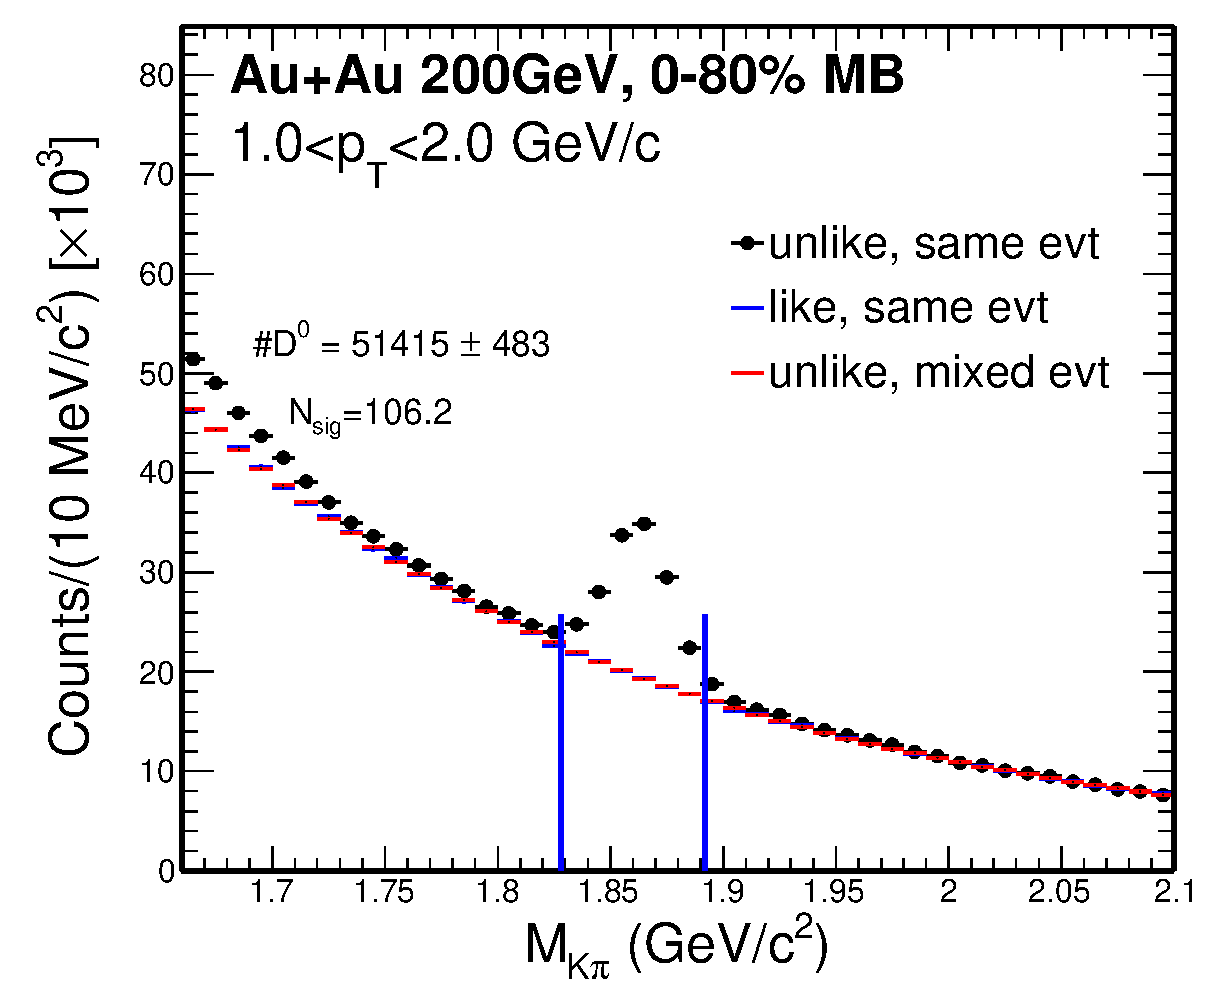
\includegraphics[keepaspectratio,width=0.6\textwidth]{fig/Mixed_cent_1_9_pt_1_2.eps}
\caption{Invariant mass distribution for foreground and two descriptions of combinatorial background in 1 < $p_T$ < 2 GeV/$c$.}
\label{fig:mixedEvent_pt1_2}
\end{figure}

\begin{figure}[htbp]
\centering
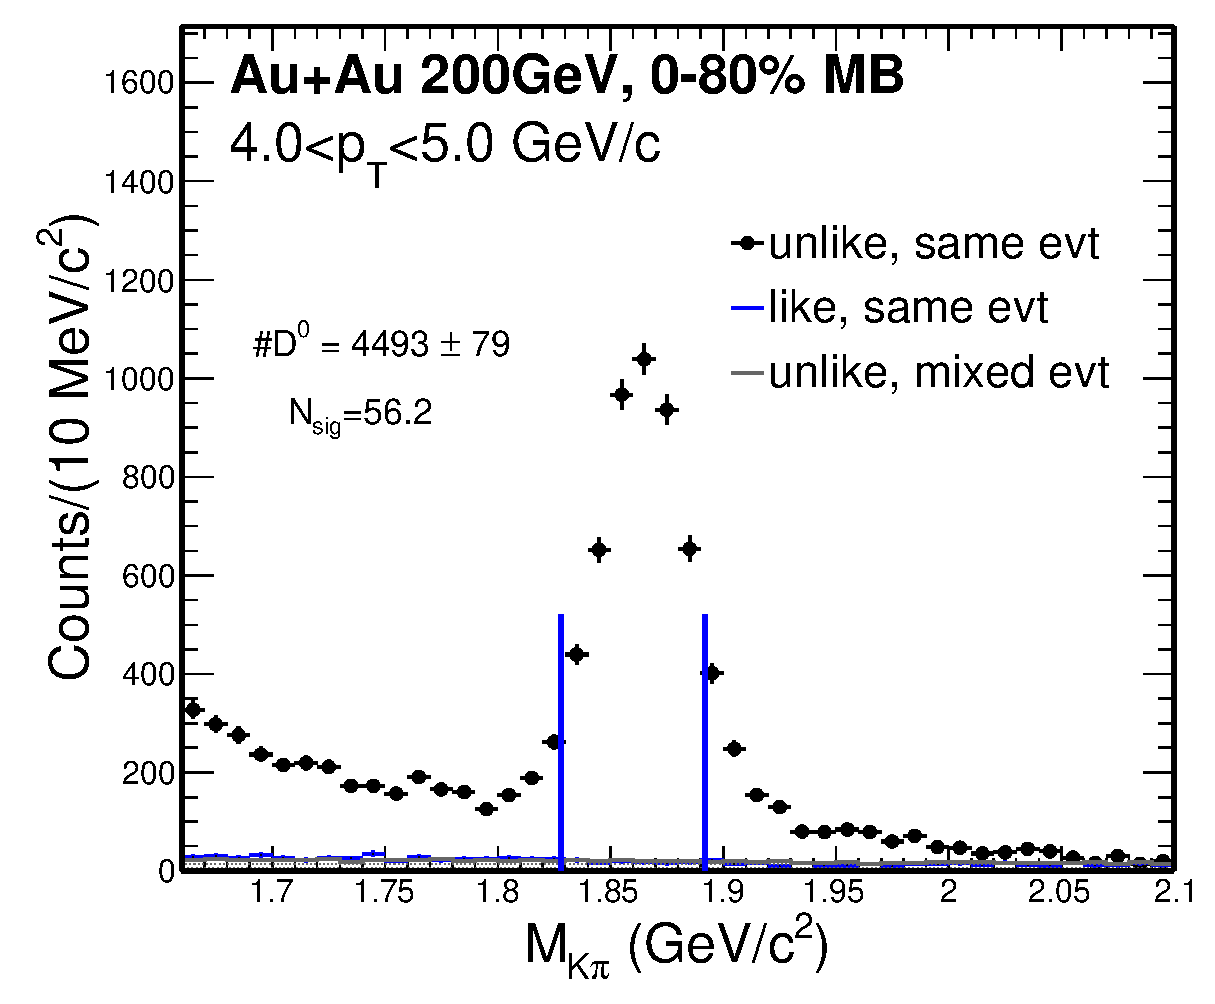
\includegraphics[keepaspectratio,width=0.6\textwidth]{fig/Mixed_cent_1_9_pt_4_5.eps}
\caption{Invariant mass distribution for foreground and two descriptions of combinatorial background in 4 < $p_T$ < 5 GeV/$c$.}
\label{fig:mixedEvent_pt4_5}
\end{figure}

There is good agreement between the two descriptions of the combinatorial background and they appear to provide an adequate description in the vicinity of the $D^0$ signal and the mixed event backgrounds have improved statistical precision.

It is interesting to observe the presence of an `excess' in the foreground, relative to all of the background curves, below roughly 1.75 GeV/$c^2$.  This so called bump was investigated using the Data Driven Fast Simulator, and will be covered briefly in the following section.

\subsection{Correlated background `bump' for $D^0$ meson}

The contributions to the invariant mass spectrum from the following $D^0$ and $D^\pm$ decays were included in a qualitative study of the correlated background: 

\begin{itemize}
\item $D^0 \rightarrow K^-\pi^+$ (B.R. 0.039)
\item $D^0 \rightarrow  K^-\pi^+\pi^0$ (B.R. 0.011)
\item $D^0 \rightarrow  K^-\rho^+ \rightarrow K^-\pi^+\pi^0$ (B.R. 0.108)
\item $D^0 \rightarrow  K^{*-}\pi^+\rightarrow K^-\pi^+\pi^0$ (B.R. 0.007)
\item $D^+ \rightarrow  K^-\pi^+\pi^+$ (B.R. 0.073 $\times$ 0.415)
\end{itemize}

The charm fragmentation ratio used is the following from ZEUS Collaboration (arXiv:hep-ex/0508019 - Table 4):

\begin{itemize}
\item f($c \rightarrow D^+$) = 0.217 
\item f($c \rightarrow D^0$) = 0.523 
\item f($c \rightarrow D^+_s$) = 0.095
\item f($c \rightarrow \Lambda^+_c$) = 0.144
\item f($c \rightarrow D^{*+}$) = 0.200
\end{itemize}

\begin{figure}[htbp]
\centering
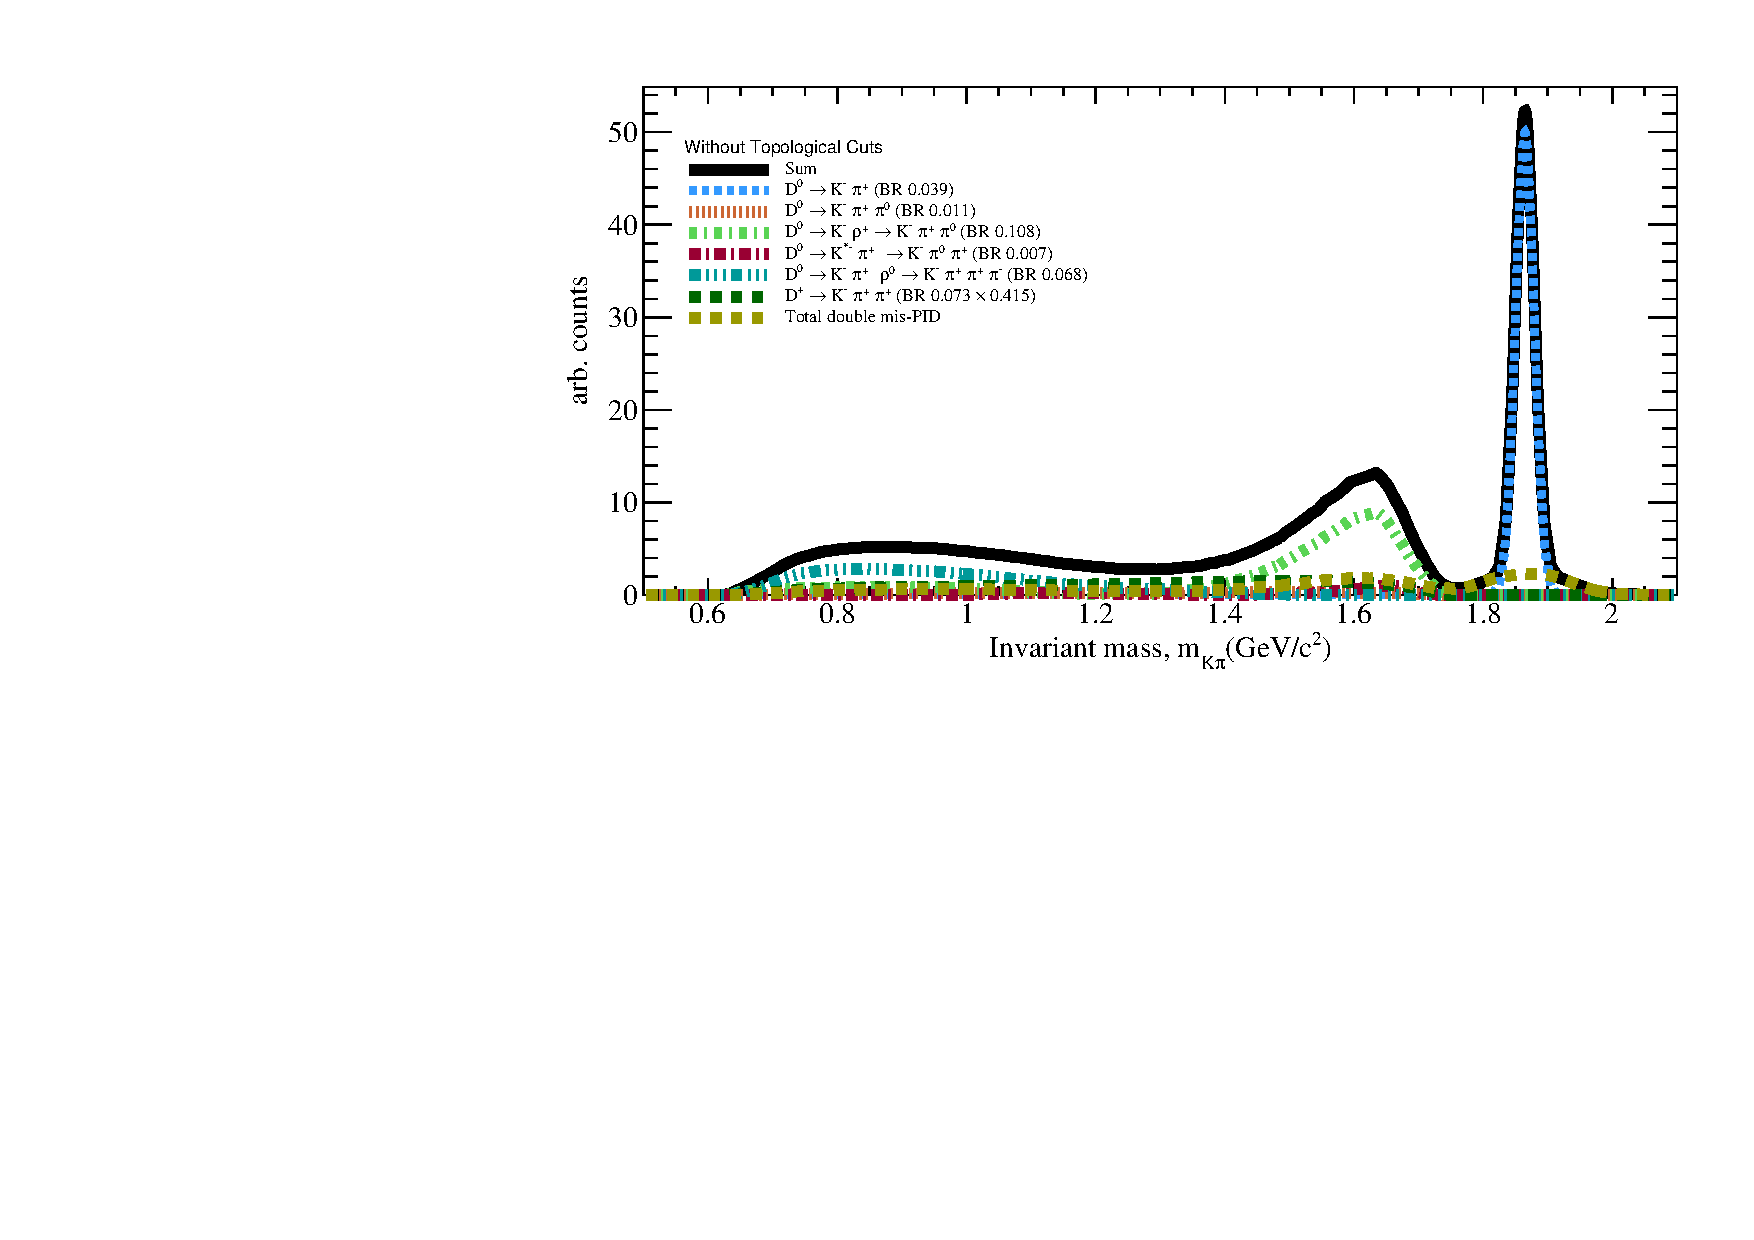
\includegraphics[keepaspectratio,width=0.7\textwidth,angle=0]{fig/D0Bump_without_topo.pdf}
\caption{Simulated contribution to the invariant mass spectrum from cocktail without topological cut}
\label{fig:cocktail1}
\end{figure}

\begin{figure}[htbp]
\centering
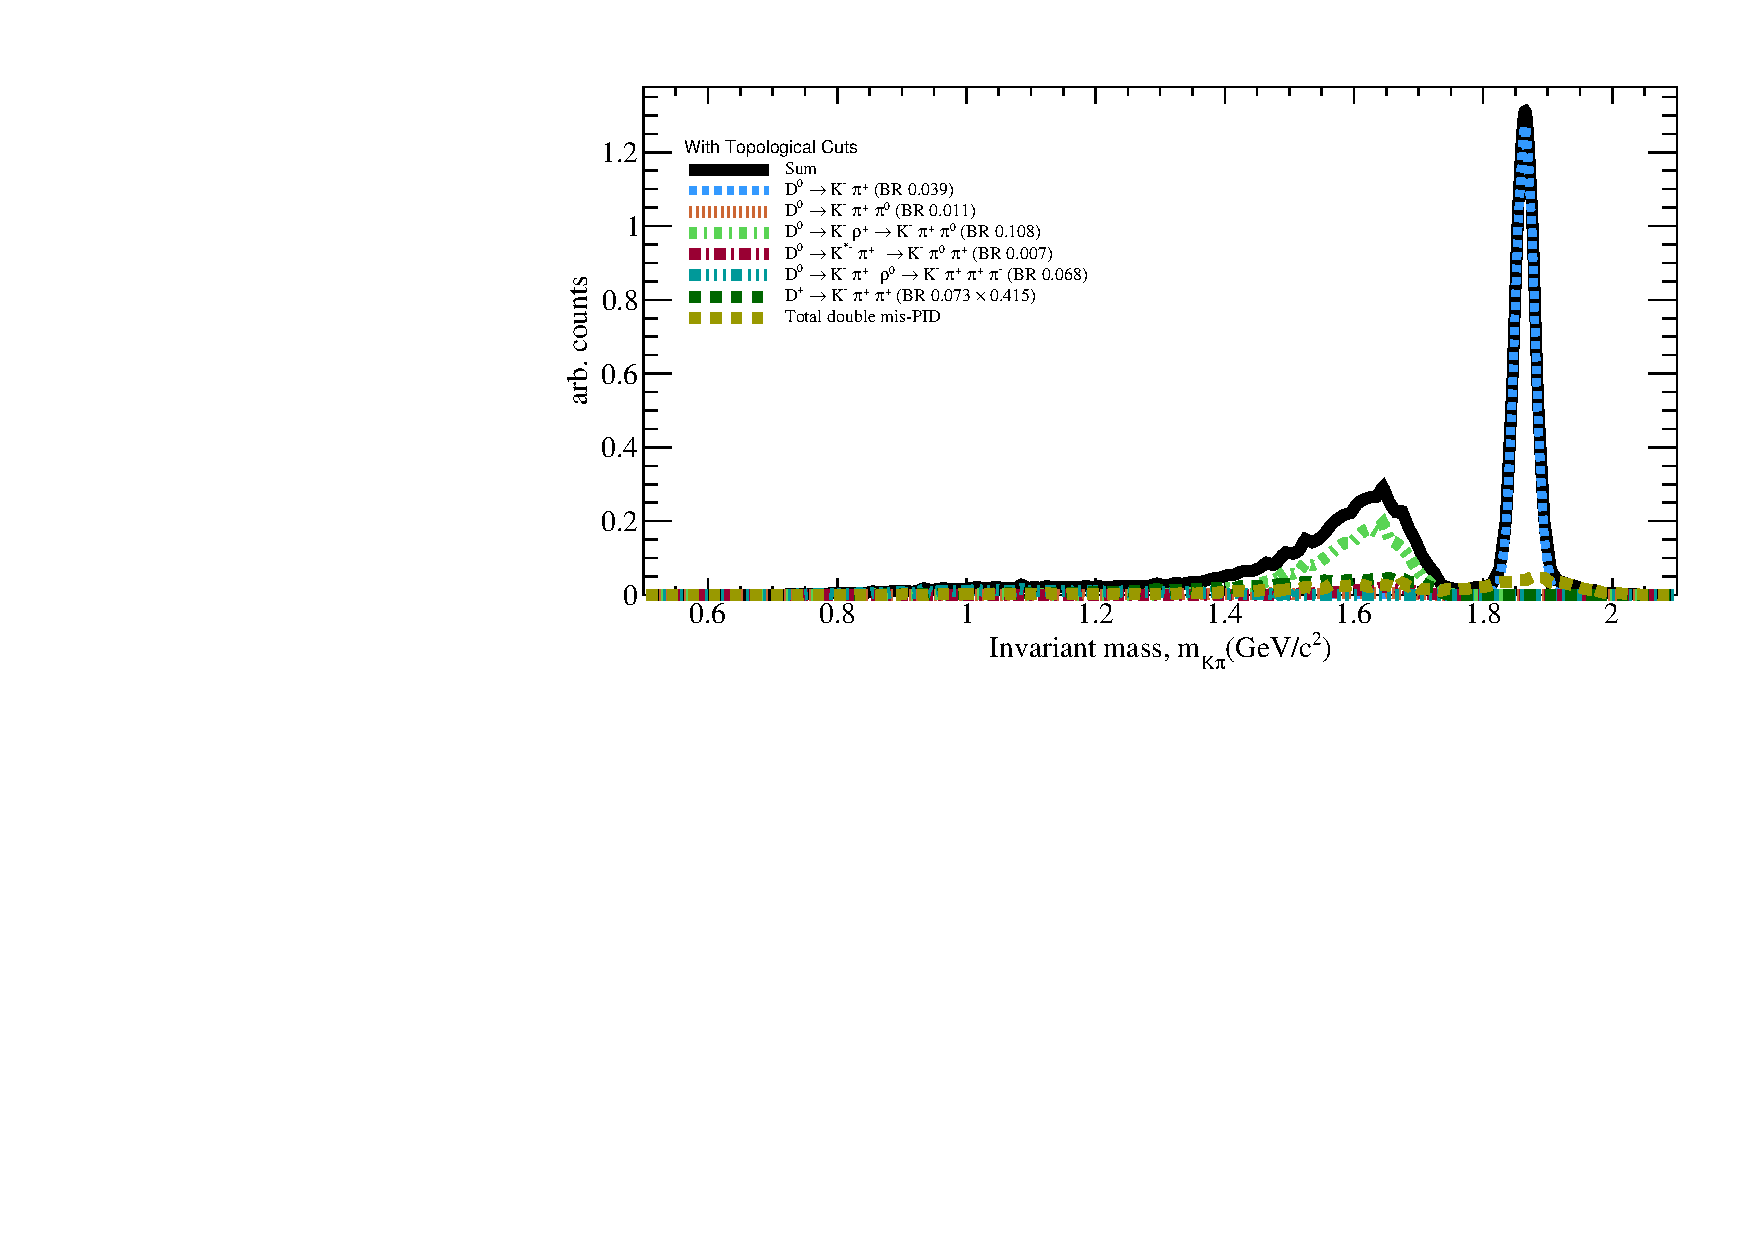
\includegraphics[keepaspectratio,width=0.7\textwidth,angle=0]{fig/D0Bump_with_topo.pdf}
\caption{Simulated contribution to the invariant mass spectrum from cocktail with topological cut}
\label{fig:cocktail2}
\end{figure}

Fig.~\ref{fig:cocktail1} and Fig.~\ref{fig:cocktail2} show the invariant mass spectrum obtained from the cocktail after scaling by the branching ratio for different decays as well as the fragmentation ratio for the different charmed meson species.

The spectrum is shown before and after the $D^0\rightarrow K\pi$ topological cuts have been applied. It is clear that the contributions from correlated background can, at least in part, account for the enhancement observed below roughly 1.7 GeV/$c^2$.

The cocktail simulation was then scaled by fitting the amplitude of the $D^0$ peak obtained from fast simulator to the signal observed in data, and the cocktail was then added to the mixed event background. Fig.~\ref{fig:bump1} and Fig.~\ref{fig:bump2} shows a comparison between the invariant mass distribution obtained from data and the spectrum obtained by combining the mixed event background and the results from the data-driven Fast-Simulator.

\begin{figure}[htbp]
\centering
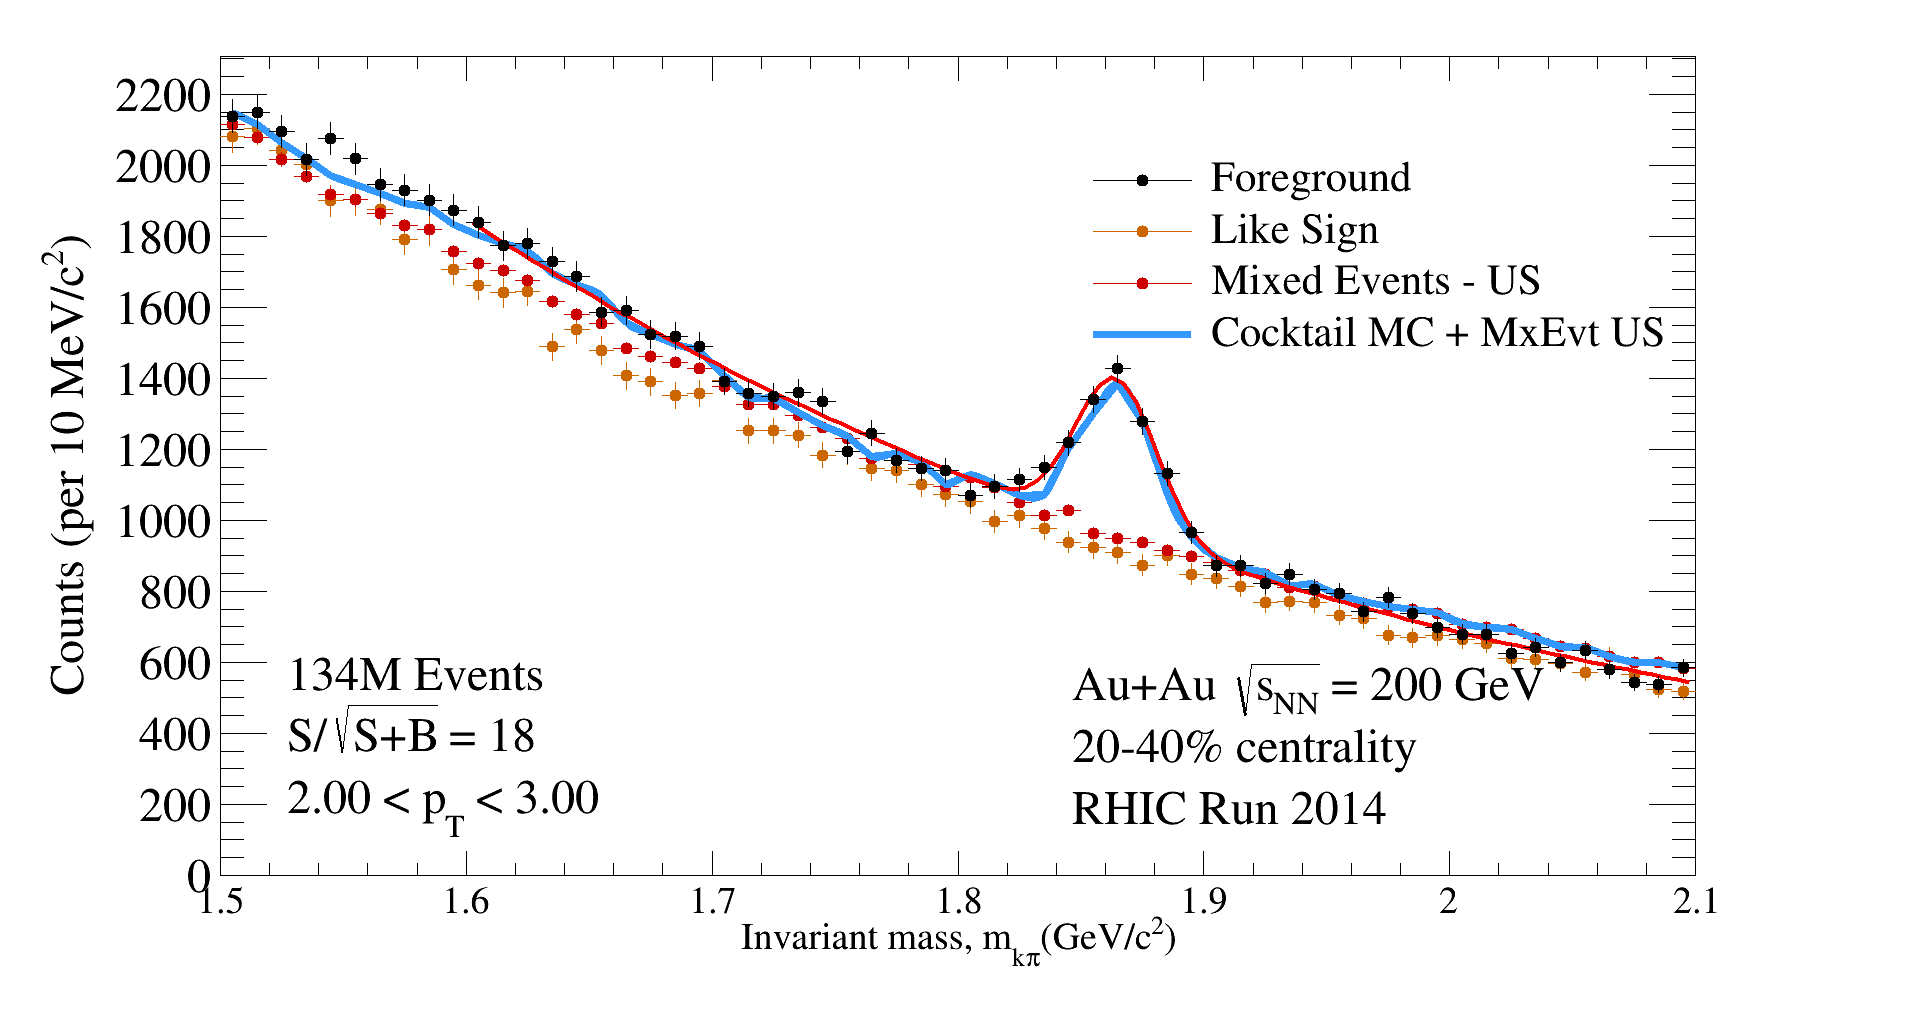
\includegraphics[keepaspectratio,width=0.7\textwidth]{fig/D0_FG_EvMxBg_coktail_2040_2_pT_3.png}
\caption{Comparison of $K\pi$ invariant mass distribution for unlike-sign (US) foreground, like-sign combinatorial background, unlike-sign (US) mixed events combinatorial background, and unlike-sign (US) mixed events combinatorial background + toy montecarlo cocktail for correlated background, for 2 < $p_T$ < 3 GeV/$c$.}
\label{fig:bump1}
\end{figure}

\begin{figure}[htbp]
\centering
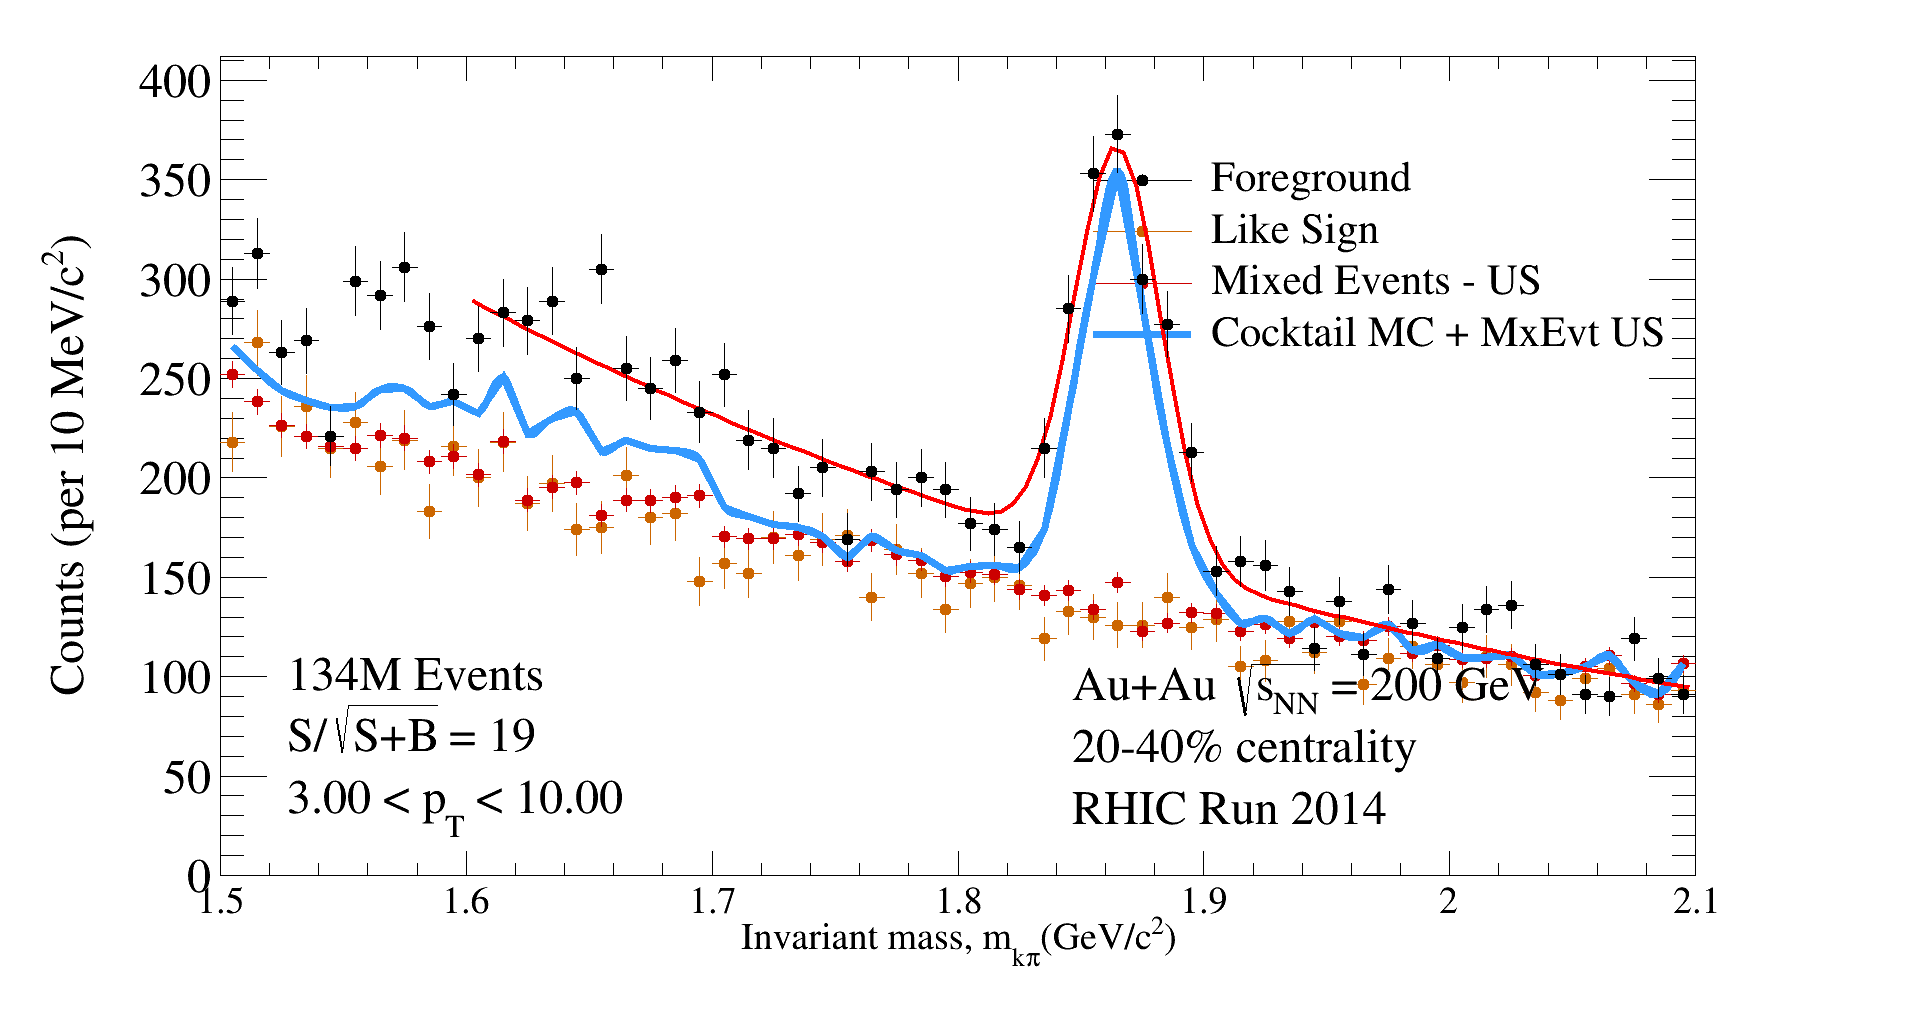
\includegraphics[keepaspectratio,width=0.7\textwidth]{fig/D0_FG_EvMcBg_cocktail_2040_3_pT_10.png}
\caption{Similar Comparison of $K\pi$ invariant mass distribution as Fig.~\ref{fig:bump1}, for 3 < $p_T$ < 10 GeV/$c$.}
\label{fig:bump2}
\end{figure}

The inclusion of correlated background sources can qualitatively describe the foreground observed, reproducing the location of the bump structure albeit underestimating the degree of enhancement itself. Furthermore, there is likely a finite contribution to the observed bump originating from jet correlations which should be included to improve on the description of the background.

It should also be noted that the studies presented here were done with an early version of the fast simulator which only included the $p_T$ and centrality dependence of sampled distributions, revisiting the studies with more differential distributions should improve on these results.

Nonetheless, the results provide confidence in a qualitative understanding on the sources of the correlated background and, what is more, suggest that the contribution from these source in the $D^0$ signal range is dominated by double mis-PID, and is nearly negligible as shown in the following sub-section.

% For the more details of the mixed-event backgrounds and the `bump' structures in the foreground, they also can be found in the $v_2$ analysis note.

\section{Efficiency Correction}
General idea.....

To obtain the real invariant mass spectrum of $D^0$ within STAR acceptance ($|\eta_{\pi}| \leq 1, |\eta_{K}| \leq 1, |Y_{K\pi}| \leq 1$), the raw spectrum should correct for the efficiency. The $K\pi$ pair efficiency within STAR acceptance is evaluated by folding the TPC related efficiency to the HFT related efficiency as shown on Eq.~\ref{effEqu}. For the TPC related tracking efficiency shows on the first term, we use STAR standard Full GEANT simulation. For the HFT related efficiency include the second and third terms which reflect to HFT acceptance and topological cuts, we developed the `Data-Driven Fast simulation' which will discuss later.

\begin{equation}
  \textup{Efficiency} \times \textup{Acceptance}  = \textup{TPC Tracking Eff} \otimes \textup{HFT Tracking Eff} \otimes \textup{Topollogy Cuts}
\label{effEqu}
\end{equation}

This formula can be written in another way when we consider the particles identification (PID) Eq.~\ref{effEqu2}. Here the PID part are able to factorized as Eq.~\ref{effEqu3}, Eq.~\ref{effEqu4}.

\begin{equation}
  \frac{\textup{HFT}}{\textup{MC}} =  \frac{\textup{TPC}_\textup{{withPID}}}{\textup{MC}} \otimes \frac{\textup{HFT}_\textup{{withPID}}}{\textup{TPC}_\textup{{withPID}}} \otimes \textup{PID}
\label{effEqu2}
\end{equation}

\begin{equation}
  \varepsilon(HFT \& PID_{TPC} \& PID_{TOF}) = \varepsilon(HFT | _{PID_{TPC} \& PID_{TOF}}) \times \varepsilon_{PID}(TPC\&TOF)
\label{effEqu3}
\end{equation}

\begin{equation}
  \varepsilon_{PID}(TPC\&TOF) = \varepsilon_{PID}(TOF | TPC) \times \varepsilon_{TPC}
\label{effEqu4}
\end{equation}

\subsection{Single Track Efficiency}

The single track efficiency losses have two contributions, the detector inefficiency and particle identification cuts. The detector efficiency includes the TPC tracking efficiency ($\varepsilon_{TPC}$) and the TOF matching efficiency ($\varepsilon_{TOF}$). The particle identification cut efficiency ($\varepsilon_{PID}$) includes the efficiencies of TOF velocity (1/$\beta$) and the $dE/dx$ selection cuts. So the single track efficiency can be derived by the Eq.~\ref{singleeff}

\begin{equation}
\varepsilon = \varepsilon_{TPC} \times \varepsilon_{TOF} \times \varepsilon_{PID}
\label{singleeff}
\end{equation}

\subsection{TPC Tracking Efficiency}

The TPC tracking efficiency ($\varepsilon_{TPC}$) is evaluated via the standard STAR embedding technique. TPC efficiency including two parts, TPC response and acceptance efficiency. The Monte Carlo (MC) tracks are embedded into the raw data to have a realistic detector occupancy environment. The raw data is randomly sampled over the entire Au+Au minimum-bias data set, while the number of embedded MC tracks is constrained to 5\% of the measured multiplicity of the real events to avoid a sizable impact on the realistic TPC tracking efficiency. The MC tracks, with flat $p_{T}$, $\eta$, and $\phi$, are generated and passed through the full GEANT simulation of the STAR detector geometry, and then mixed with the real data . The mixed signals are processed using the same procedures as real data.  The quality assurance is made to ensure the MC simulation reproduces the real data before studying the TPC tracking efficiency (Embedding QA). The TPC tracking efficiency is derived by taking the ratio of the number of reconstructed MC tracks ($N_{rec}$), satisfying the track quality cuts used in the data analysis, over the number of embedded MC tracks ($N_{emb}$), as shown in Eq.~\ref{tpceff}

\begin{equation}
\varepsilon_{TPC} = \frac{N_{rec}\;(nHitsFit\geq20\;\&\;dca\leq1\;\&\;|\eta|\leq1\;\&\;nCommonHits > 10)}{N_{emb}\;(|\eta|\leq1)}
\label{tpceff}
\end{equation}

The TPC tracking efficiency in Run14 Au+Au collisions at 200 GeV is shown below. Fig ~\ref{fig:mpion} shows the TPC tracking efficiency for pion plus from four different classifications, from up to down, the centrality is from the most peripheral to most central collision. As we see, in the most central top 0-5\% collisions, due to the large occupancy the TPC tracking efficiency is much lower than the central one. Fig. ~\ref{fig:mkaon} shows the same plot for kaon minus. The Kaon can be decay inside TPC, that's the reason the TPC tracking efficiency is lower than pion.

\begin{figure}[htbp]
\begin{minipage}[htbp]{0.52\linewidth}
\centering
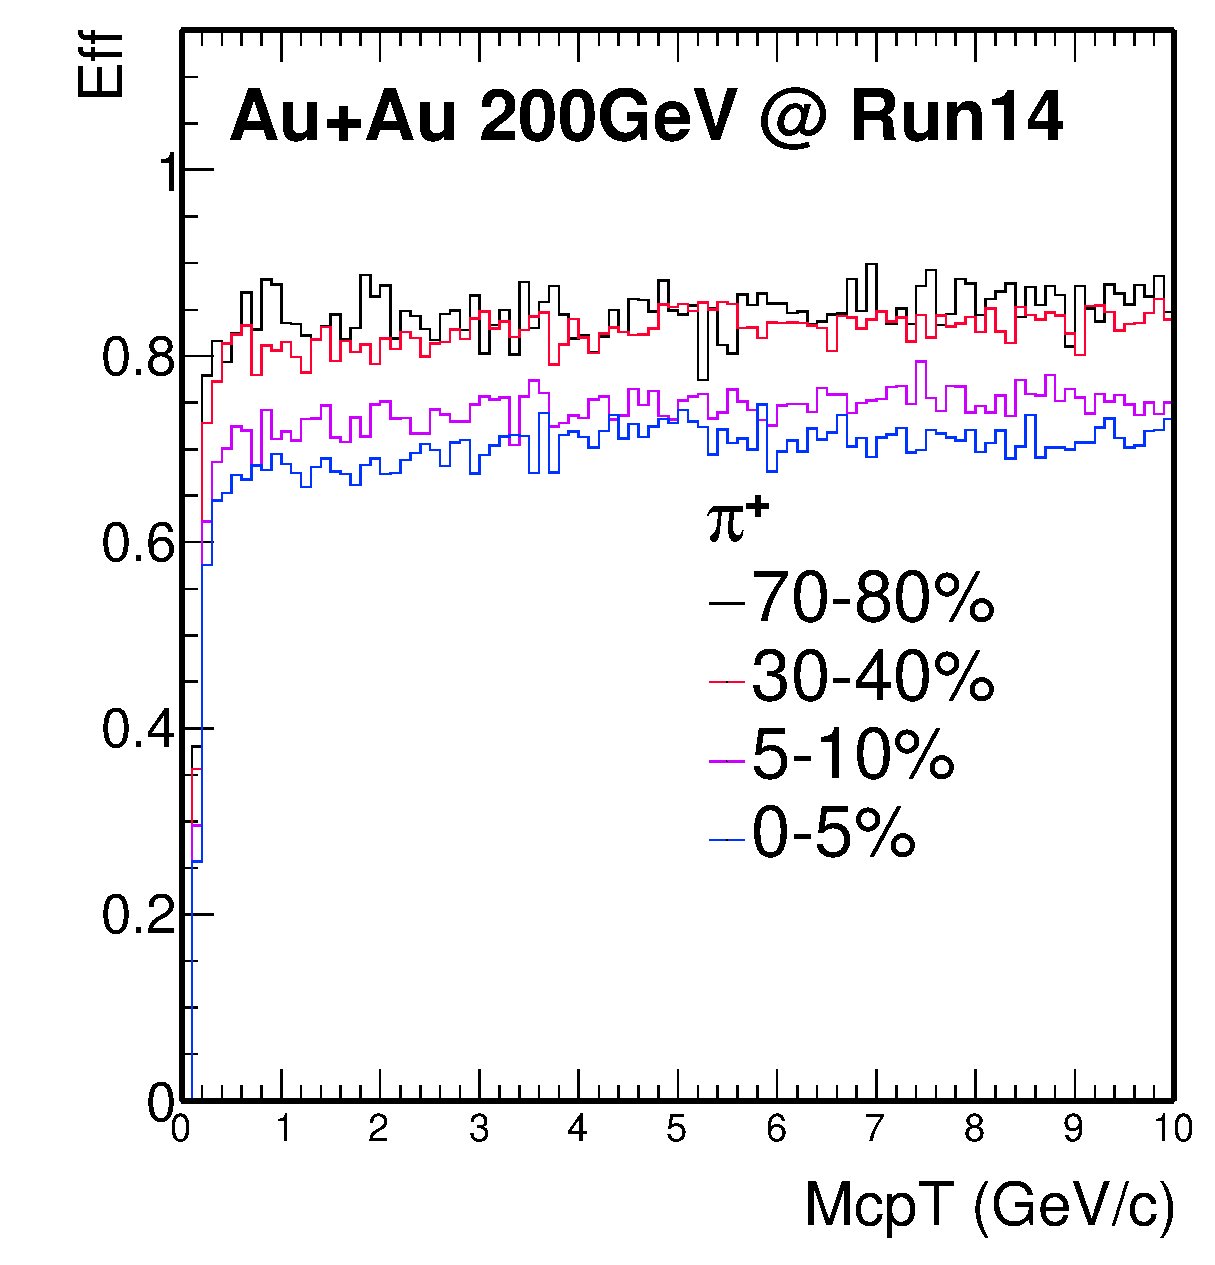
\includegraphics[width=1.0\textwidth]{fig/pion.eps}
\caption{TPC tracking efficiency in Run14 Au+Au collisions at 200 GeV for Pion. \label{fig:mpion}}
\end{minipage}
\hfill
\begin{minipage}[htbp]{0.52\linewidth}
\centering
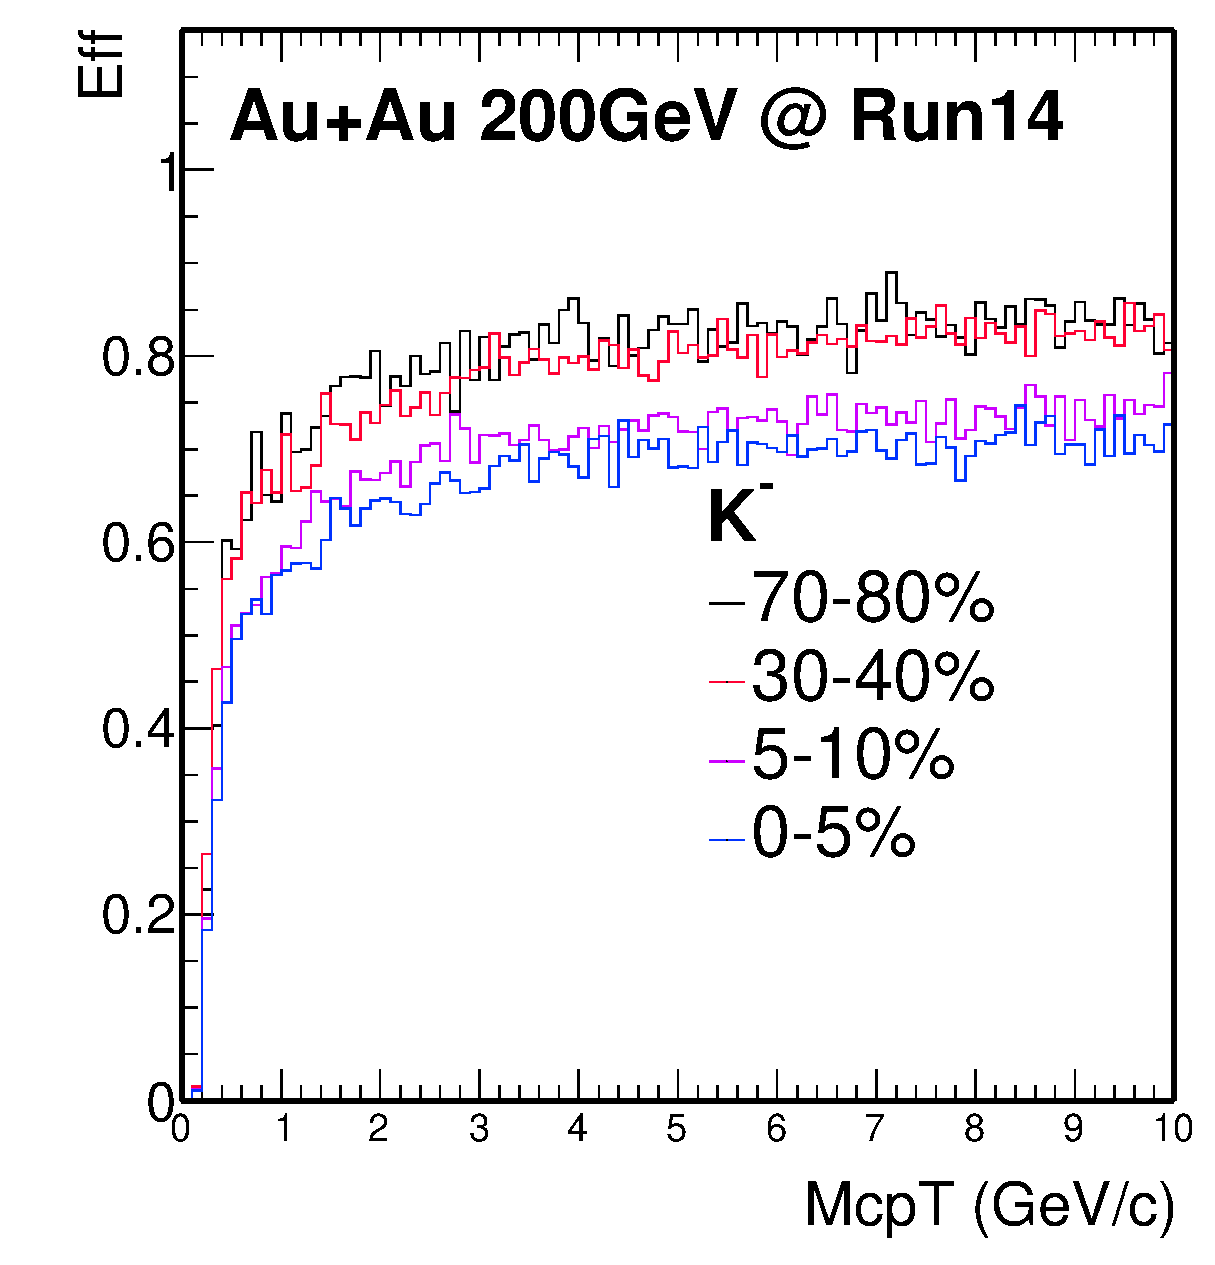
\includegraphics[width=1.0\textwidth]{fig/kaon.eps} 
\caption{TPC tracking efficiency in Run14 Au+Au collisions at 200 GeV for Kaon. \label{fig:mkaon}}
\end{minipage}
\end{figure}

\subsection{TOF Matching Efficiency}

For the $D^0$ analysis, we use the hybrid PID for TOF. Which means when TOF is available we use TOF and TPC, when it's not available we just use TPC. The TOF matching efficiency ($\varepsilon_{TOF}$), including the TOF response and the acceptance difference between the TPC and TOF, is evaluated by the real data. It can be calculated by comparing the number of qualified tracks matched with the TOF (with $\beta$ > 0, $N_{matched}$) over  the number of qualified tracks ($N_{TPC}$).

\begin{figure}[htbp]
\begin{minipage}[htbp]{0.52\linewidth}
\centering
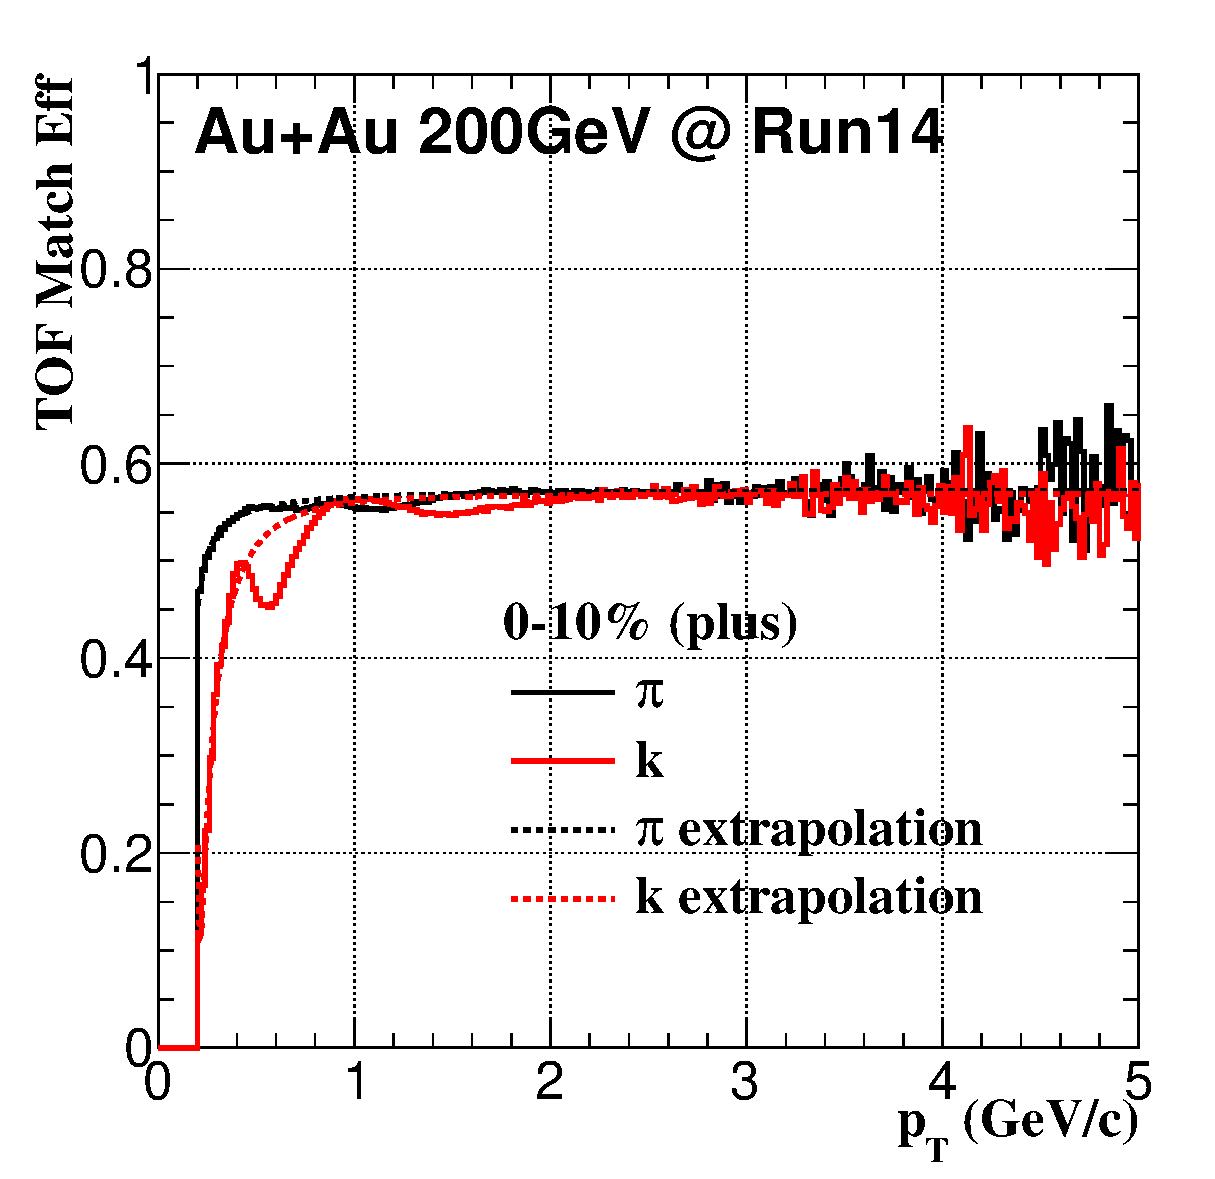
\includegraphics[width=1.0\textwidth]{fig/tofMatchEff_Run14_Fit_cent1.eps}
\caption{TOF match efficiency in Run14 Au+Au collisions at 200 GeV for positive charge particle in 0-10\%. \label{fig:mtof010}}
\end{minipage}
\hfill
\begin{minipage}[htbp]{0.52\linewidth}
\centering
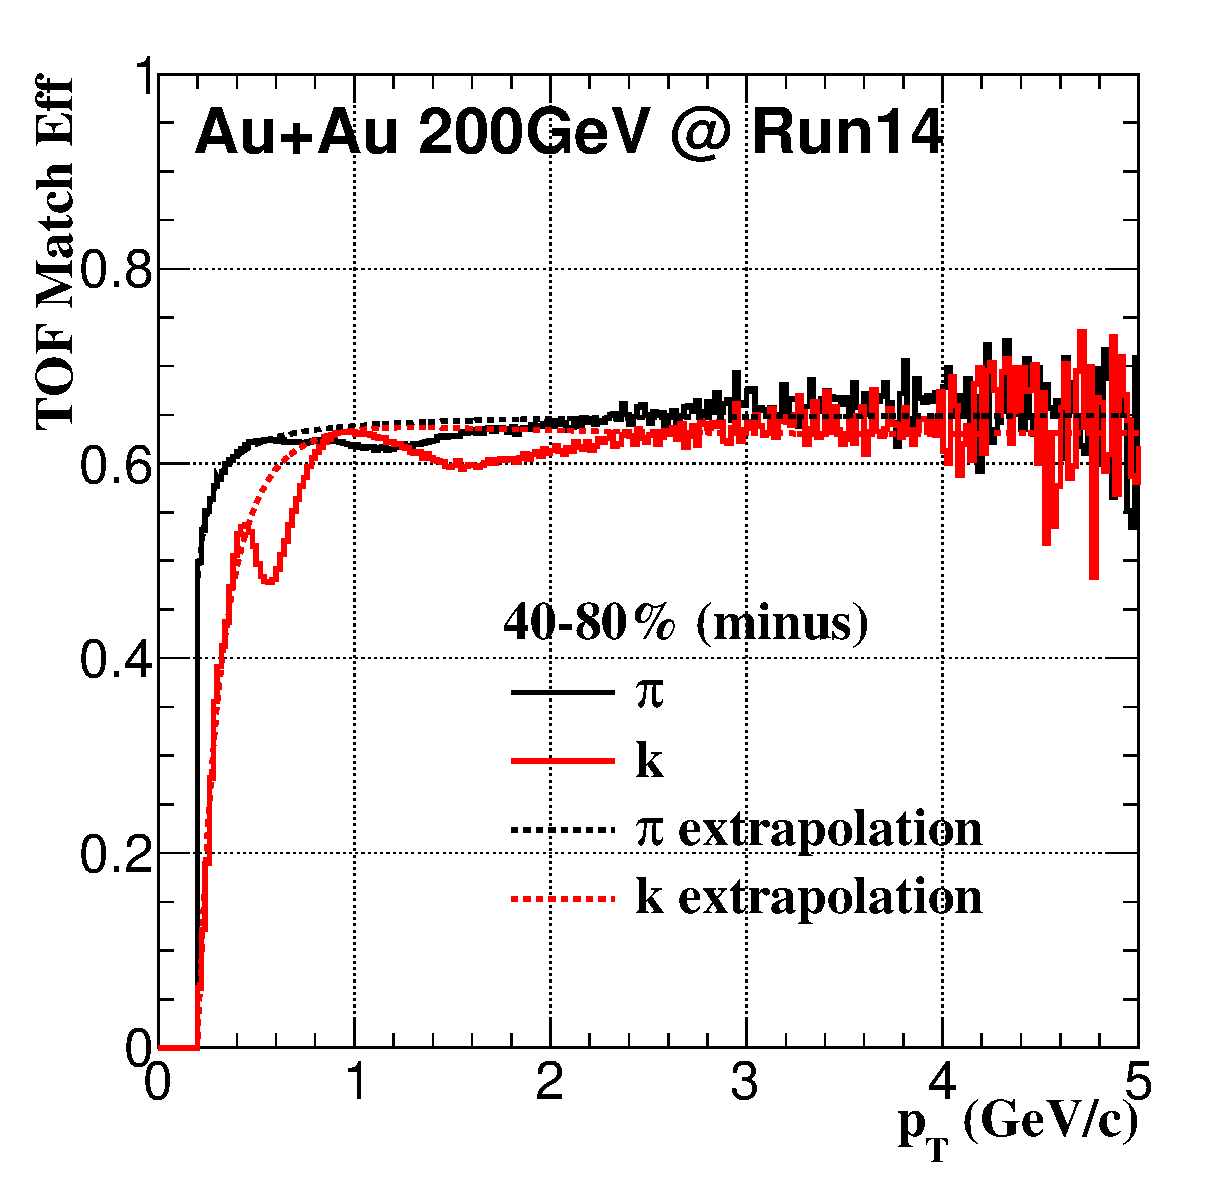
\includegraphics[width=1.0\textwidth]{fig/tofMatch_minus_Eff_Run14_Fit_cent3.eps} 
\caption{TOF match efficiency in Run14 Au+Au collisions at 200 GeV for negative charge particle in 40-80\%. \label{fig:mtof4080}}
\end{minipage}
\end{figure}


Fig.~\ref{fig:mtof010} shows the TOF match efficiency in Run14 Au+Au collisions at 200 GeV for positive charge particles such as $\pi^{+}$,$K^{+}$ in the centrality 0-10\%. Fig.~\ref{fig:mtof4080} shows the same plots for negative charge particles in the centrality from 40-80\%. For the pion TOF match efficiency, the tread is much smooth compare to kaon. As we see, there are some deep for the TOF match efficiency at some certain $p_{T}$ range from kaon, such as kaon in the $p_{T}$ around 0.6 GeV/$c$. This effect was studied using Hijing simulation, it's found that this is due to the hadron contaminations. 

Fig.~\ref{fig:tpck2} shows the $n\sigma_{K}$ distributions from Hijing in the $p_{T}$ range from 0.5 - 0.7 GeV/$c$. The solid lines are for particles from TPC , and the dashed lines are for particles also include TOF match information. The total yield was scaled to have the same number of pions for this comparison, since the TOF matching have $\sim$30-40\% efficiency lost. In a simple case, if we select kaons with the cut $|n\sigma_{K}| < 1 $, after the requiring of TOF match,the width of this $n\sigma_{K/\pi}$ distribution changed, and the contaminations from pions are reduced. As what we see the dashed black line have less contributions to the kaons peak within $|n\sigma_{K}| < 1$ compare to the solid black line. We also checked this effect in the other $p_{T}$ range such as 0.2 - 0.5 GeV/$c$ and 1.0 - 1.5 GeV/$c$ as shown in Fig.~\ref{fig:tpck1} and Fig.~\ref{fig:tpck3}. This effect is neglectable in the low $p_{T}$ range 0.2 - 0.5 GeV/$c$ since the TPC can well separate pions and kaon. In the high $p_{T}$ range, the dE/dex are overlap with each other for kaon and pion, it's not able to distinguish them only use TPC.

\begin{figure}[htbp]
\centering
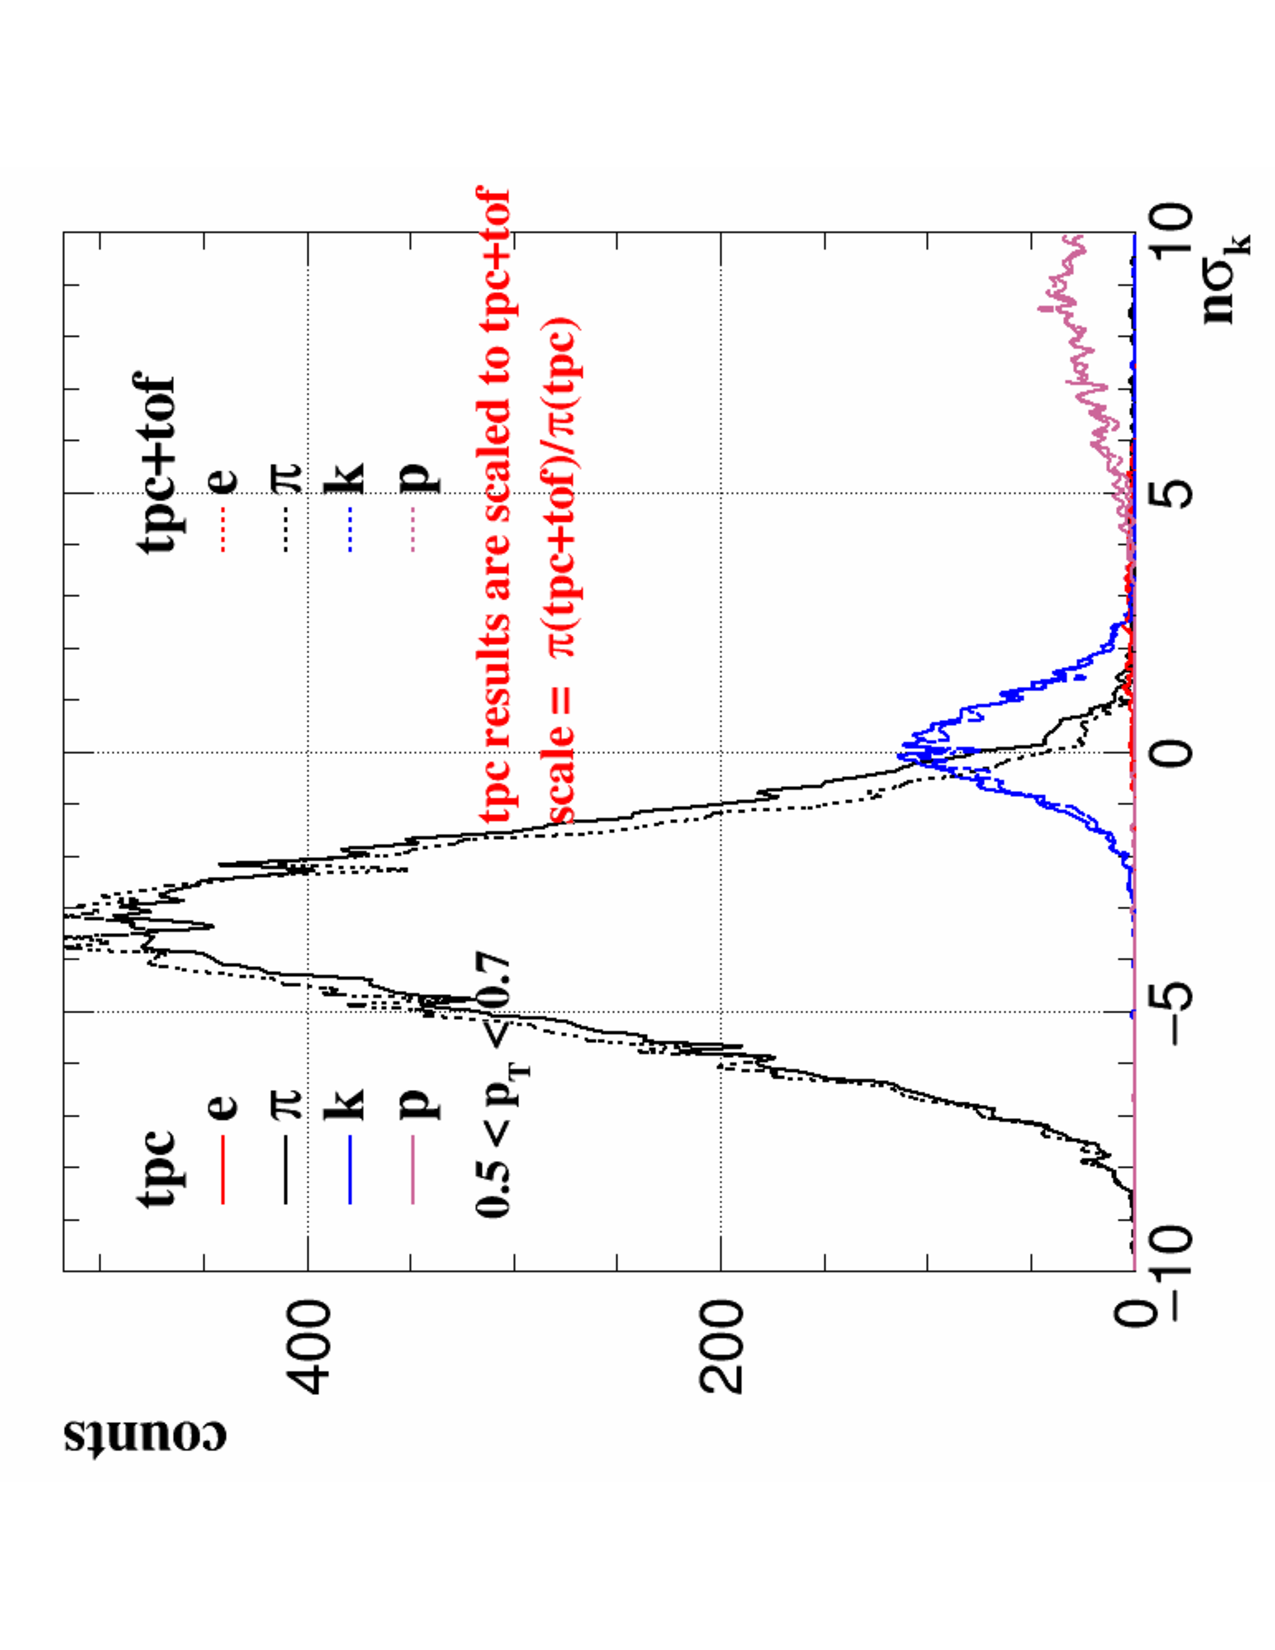
\includegraphics[keepaspectratio,width=0.6\textwidth,angle=-90]{fig/tofMatch_Hijing_nSigmaK.pdf}
\caption{$n\sigma_{K}$ distributions for 0.5 < $p_T$ < 0.7 GeV/$c$. The solid lines are from TPC and dashed lines are from TPC + TOF.}
\label{fig:tpck2}
\end{figure}

\begin{figure}[htbp]
\begin{minipage}[htbp]{0.52\linewidth}
\centering
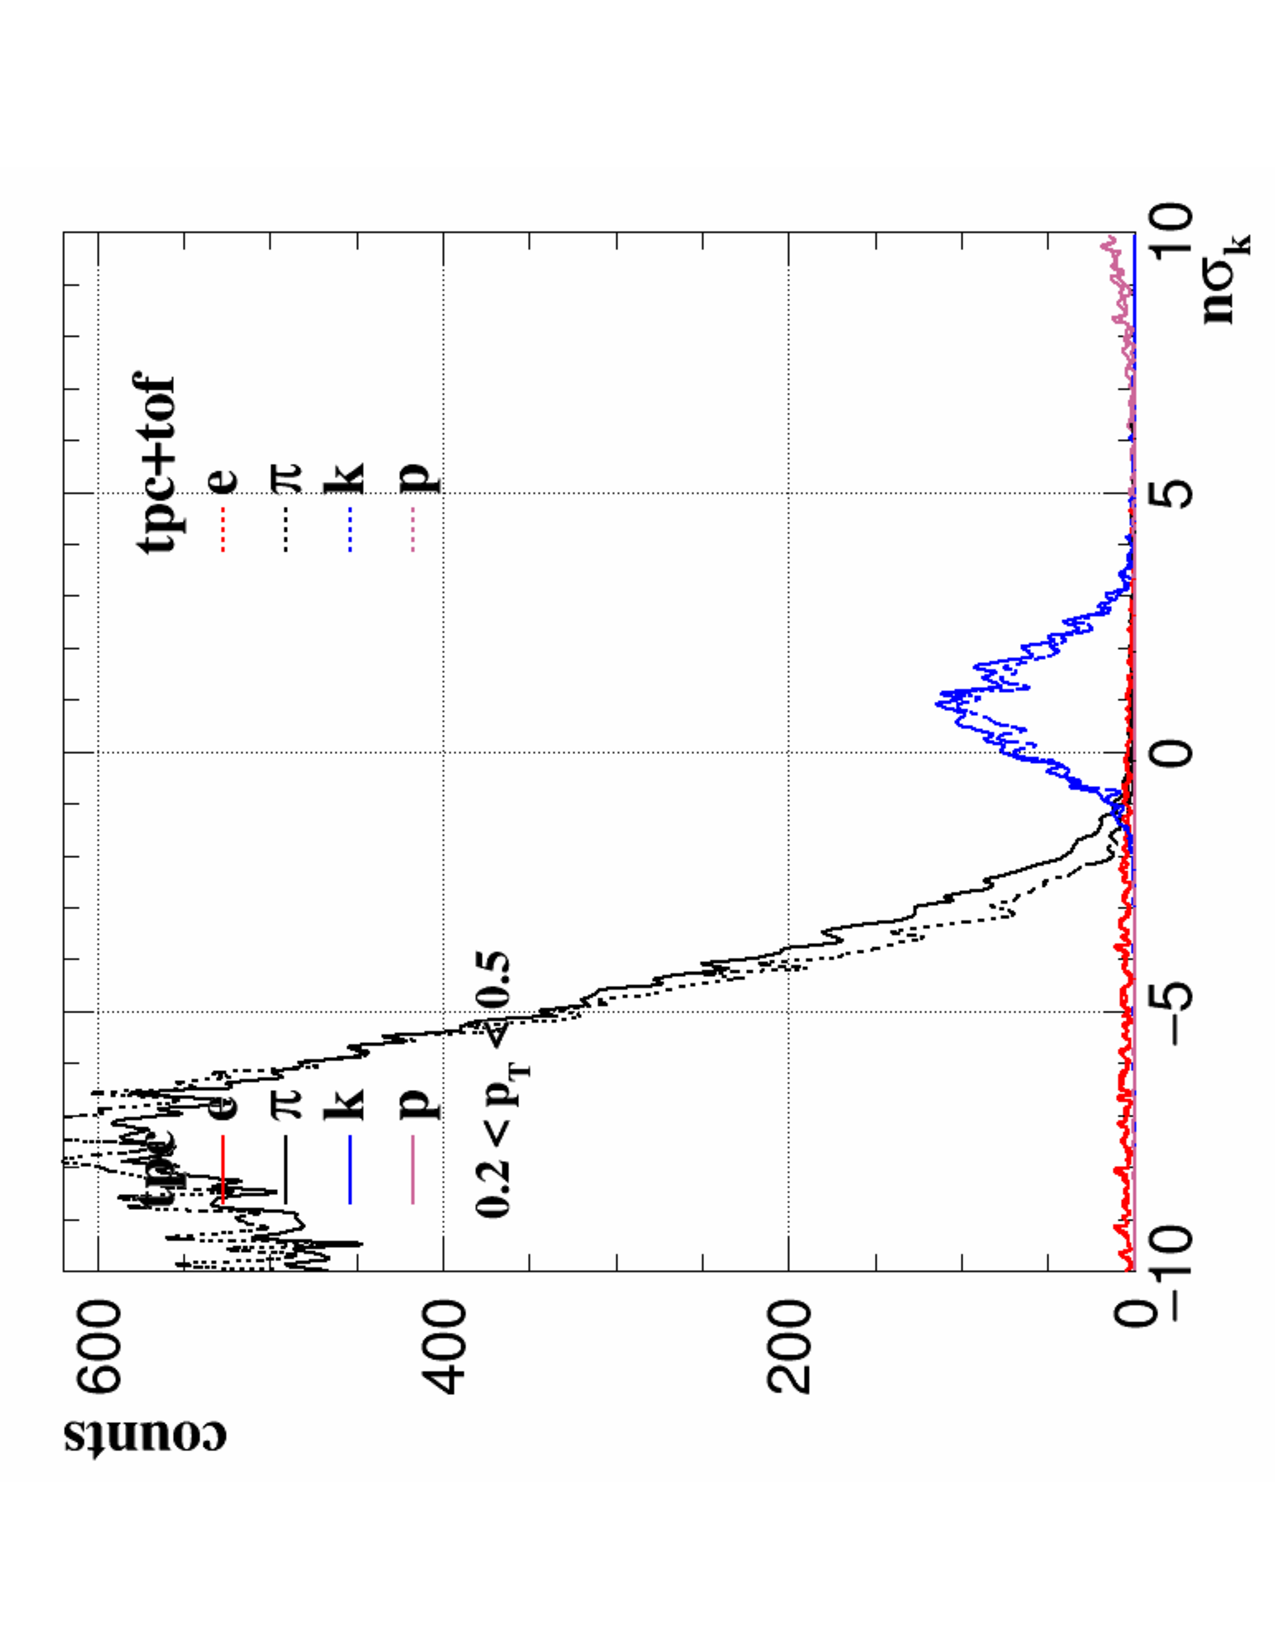
\includegraphics[width=1.0\textwidth,angle=-90]{fig/tofMatch_Hijing_nSigmaK1.pdf}
\caption{$n\sigma_{K}$ distributions for 0.2 < $p_T$ < 0.5 GeV/$c$. The solid lines are from TPC and dashed lines are from TPC + TOF.\label{fig:tpck1}}
\end{minipage}
\hfill
\begin{minipage}[htbp]{0.52\linewidth}
\centering
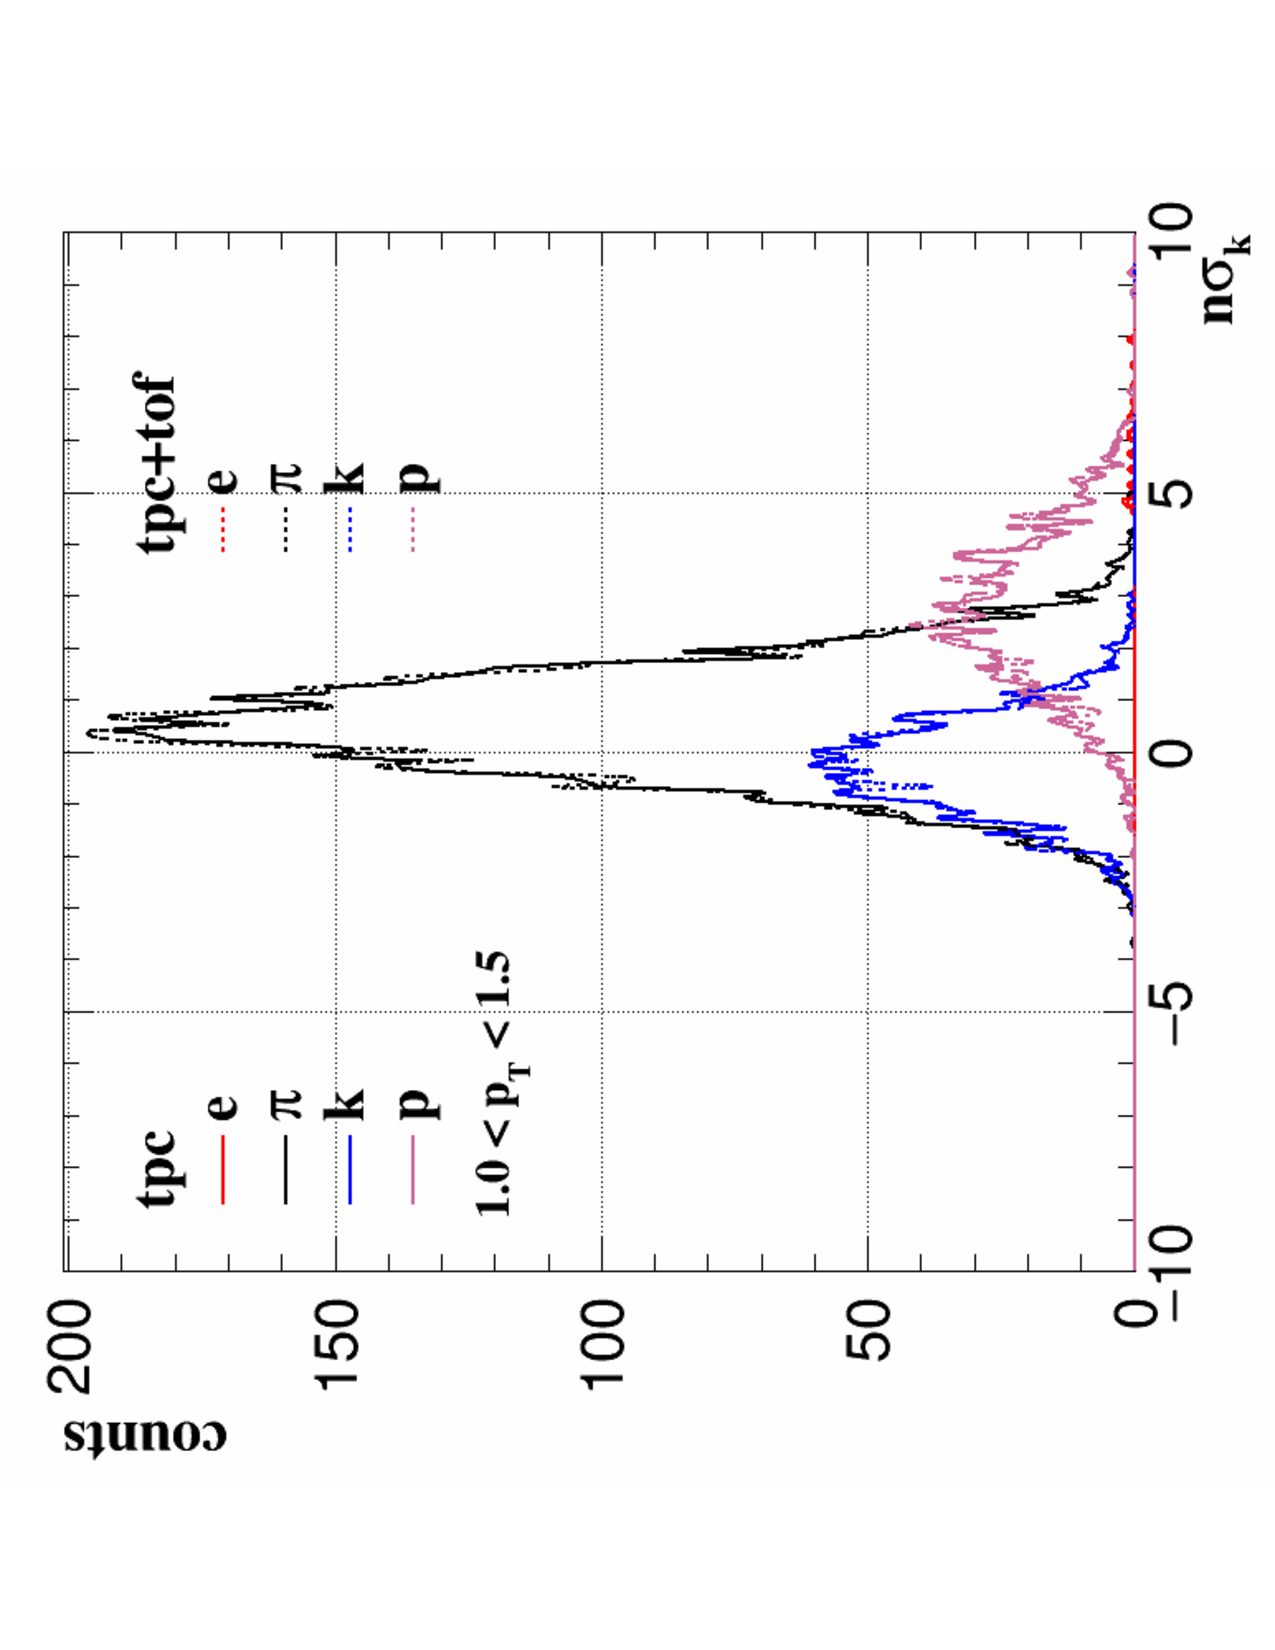
\includegraphics[width=1.0\textwidth,angle=-90]{fig/tofMatch_Hijing_nSigmaK2.pdf} 
\caption{$n\sigma_{K}$ distributions for 1.0 < $p_T$ < 1.5 GeV/$c$. The solid lines are from TPC and dashed lines are from TPC + TOF.\label{fig:tpck3}}
\end{minipage}
\end{figure}

\subsection{PID Cut Efficiency}
\label{pideff}
The particle identification cut efficiency ($\varepsilon_{PID}$) includes two components: the TOF velocity ($1/\beta$) cut efficiency and $dE/dx$ cut ($n\sigma_{K/\pi}$) efficiency. Pure pions and kaons sample are used to evaluate the TOF velocity cut efficiency and TPC $n\sigma_{K/\pi}$ cut efficiency. Fig.~\ref{fig:ksmass} shows the $\pi\pi$ pairs invariant mass distributions. The black line is the unlikesign foreground, and the red line is background using likesign method. With this $K_{s}^{0}$ candidates, we can statistical extract the pure pion sample for the PID efficiency study. Fig.~\ref{fig:phimass} shows the $KK$ pairs invariant mass distributions. Still with the unlikesign and likesign method, the $\Phi$ meson candidates are reconstructed, and we can statistical extract the pure kaon sample for the PID efficiency study.

\begin{figure}[htbp]
\begin{minipage}[htbp]{0.52\linewidth}
\centering
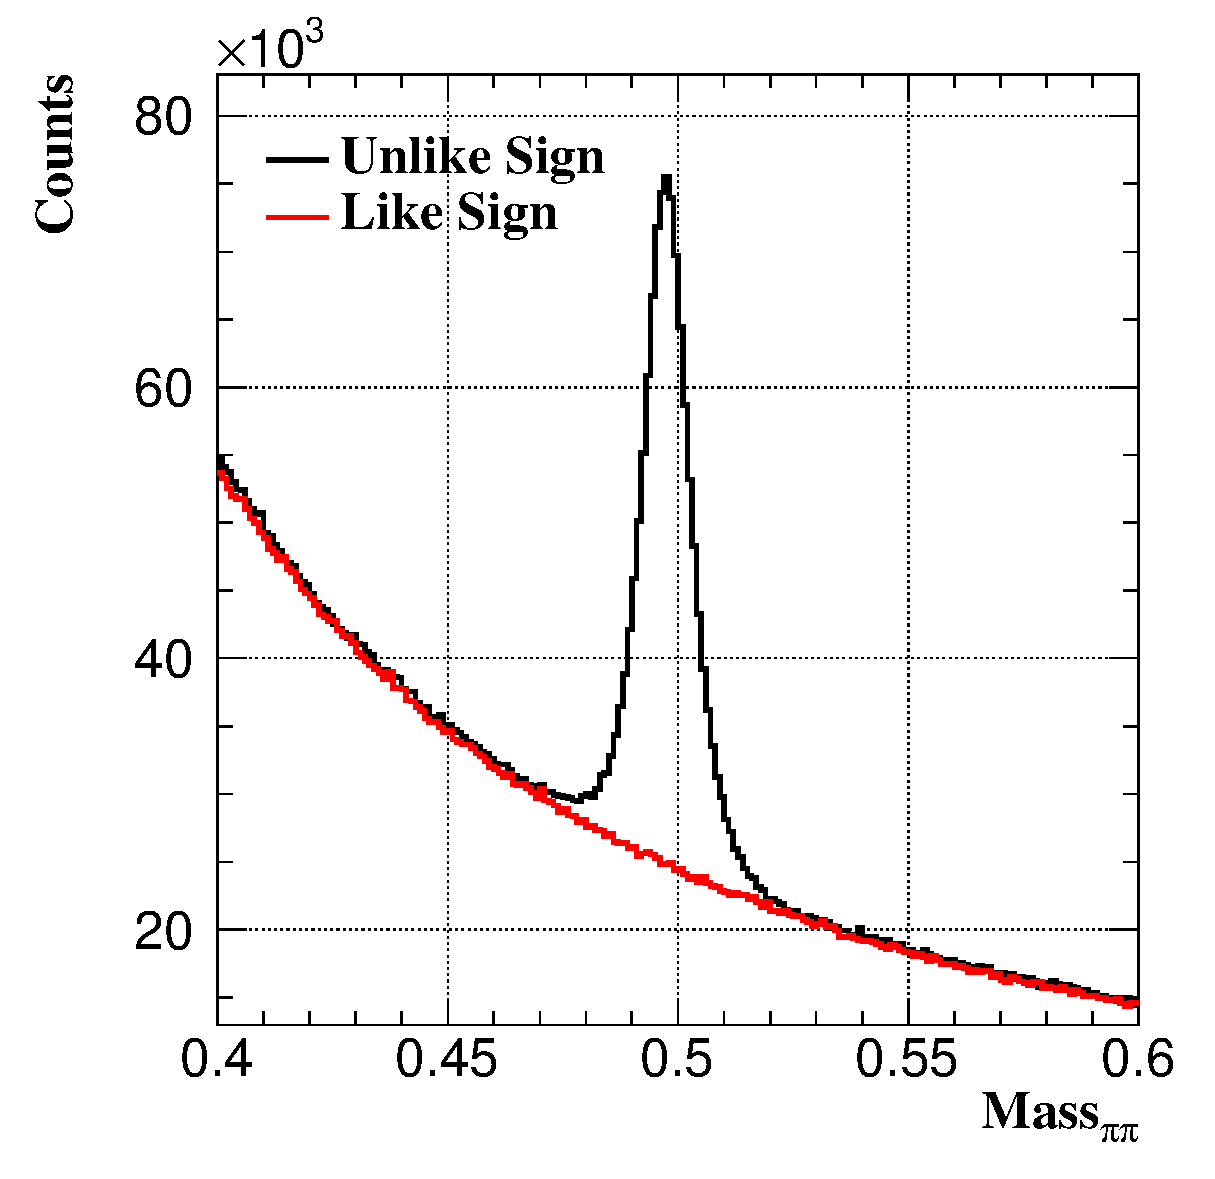
\includegraphics[width=1.0\textwidth]{fig/massKshort.eps}
\caption{The $\pi\pi$ pairs invariant mass distributions. The black line is the unlikesign foreground, and the red line is background using likesign method. \label{fig:ksmass}}
\end{minipage}
\hfill
\begin{minipage}[htbp]{0.52\linewidth}
\centering
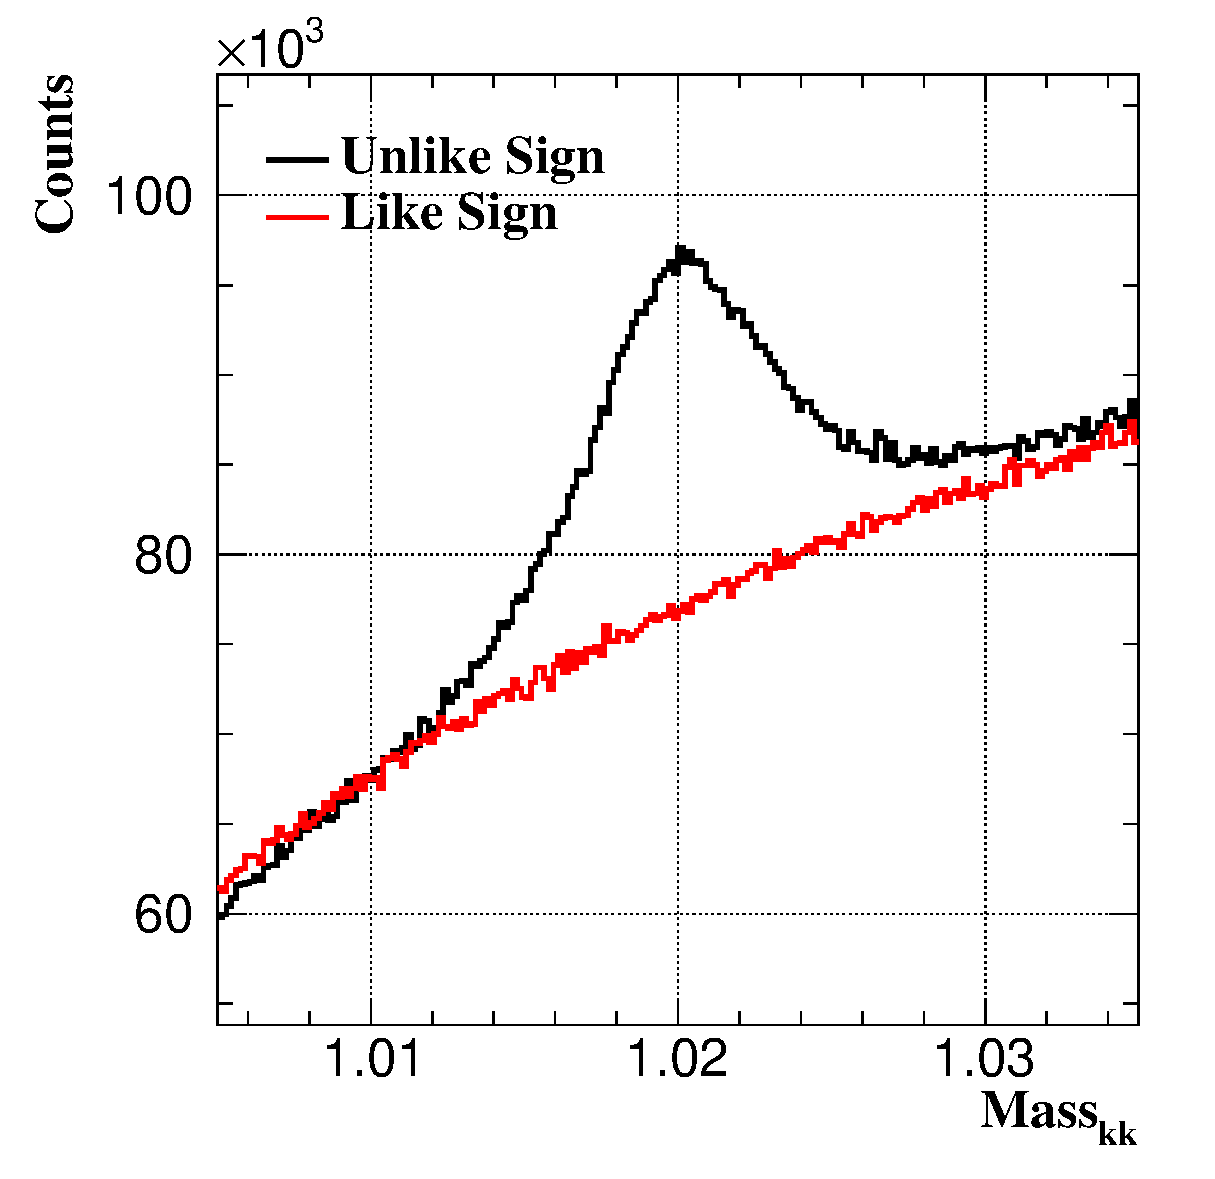
\includegraphics[width=1.0\textwidth]{fig/massPhi.eps} 
\caption{The $KK$ pairs invariant mass distributions. The black line is the unlikesign foreground, and the red line is background using likesign method. \label{fig:phimass}}
\end{minipage}
\end{figure}

\subsubsection{$n\sigma_{K/\pi}$ Cut Efficiency}

The $n\sigma_{K/\pi}$ cut efficiency is derived from the Gaussian fit using those pure samples. The $n\sigma_{K/\pi}$ distributions are fitted with Gaussian function, the mean value and sigma value are plotted as Fig.~\ref{fig:pionmean} and Fig.~\ref{fig:pionsigma}. With these mean and sigma distributions, assuming they follow the Gaussian function, for example, Fig.~\ref{fig:pionnsigmaeff} depicts the $n\sigma_{\pi}$ cut efficiency in Run14 Au + Au collisions at 200 GeV for pions. For kaons, we use the same method extracting this $n\sigma_{K}$ cut efficiency.

\begin{figure}[htbp]
\begin{minipage}[htbp]{0.5\linewidth}
\centering
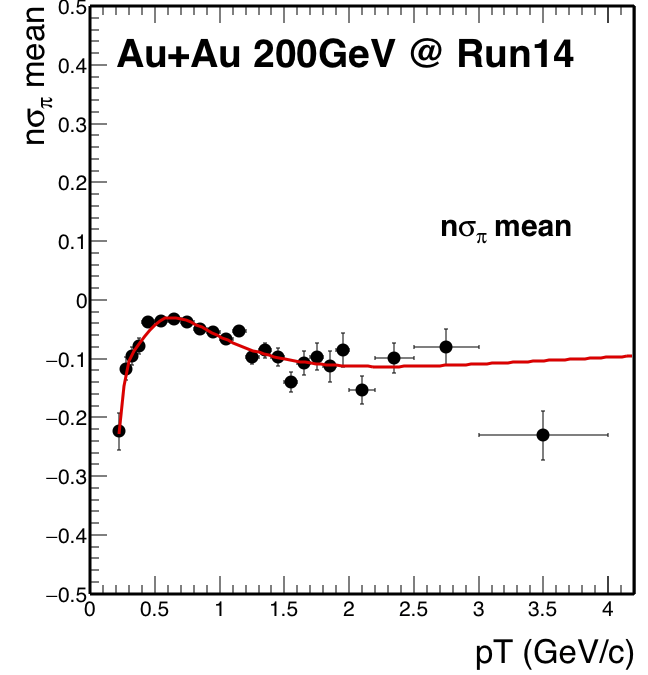
\includegraphics[width=1.0\textwidth]{fig/nSigPion_mean.png}
\caption{The mean value of $n\sigma_{\pi}$ distributions vs momentum. The red line is fitted function with polynomial function. \label{fig:pionmean}}
\end{minipage}
\hfill
\begin{minipage}[htbp]{0.5\linewidth}
\centering
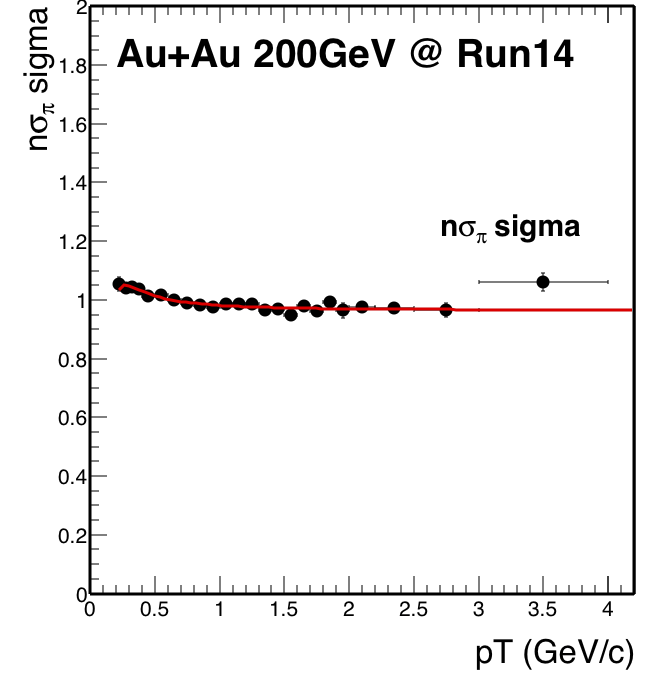
\includegraphics[width=1.0\textwidth]{fig/nSigPion_sigma.png}
\caption{The sigma value of $n\sigma_{\pi}$ distributions vs momentum. The red line is fitted function with polynomial function. \label{fig:pionsigma}}
\end{minipage}
\end{figure}

\begin{figure}[htbp]
\centering
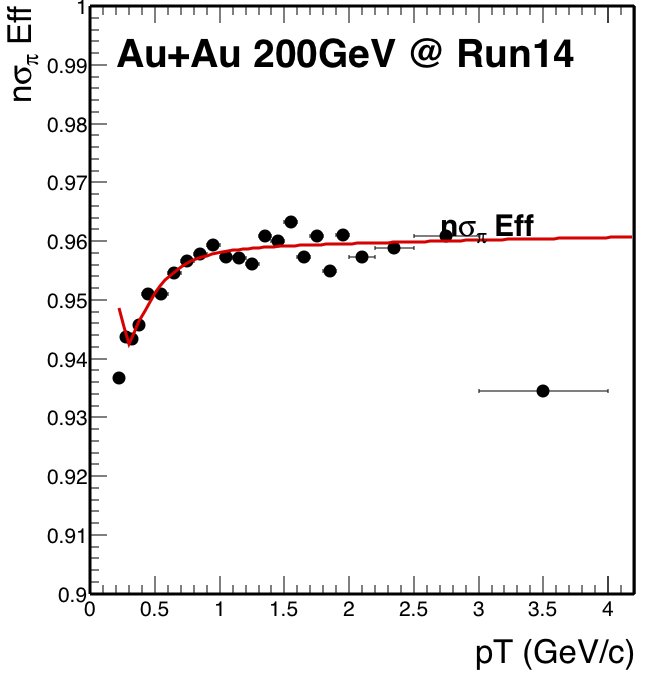
\includegraphics[keepaspectratio,width=0.55\textwidth]{fig/nSigPion_Eff.png}
\caption{$n\sigma_{\pi}$ cut efficiency along with momentum. Red line is the fitted polynomial function}
\label{fig:pionnsigmaeff}
\end{figure}

\subsubsection{$1/\beta$ Cut Efficiency}
The $1/\beta$ cut efficiency is also derived from the Gaussian fit using those pure samples. The efficiency is very high since the $1/\beta$ cut is very loose, it's almost $\sim$100\% for this analysis as shown on Fig.~\ref{fig:piontofeff} and Fig.~\ref{fig:kaontofeff}.

\begin{figure}[htbp]
\begin{minipage}[htbp]{0.5\linewidth}
\centering
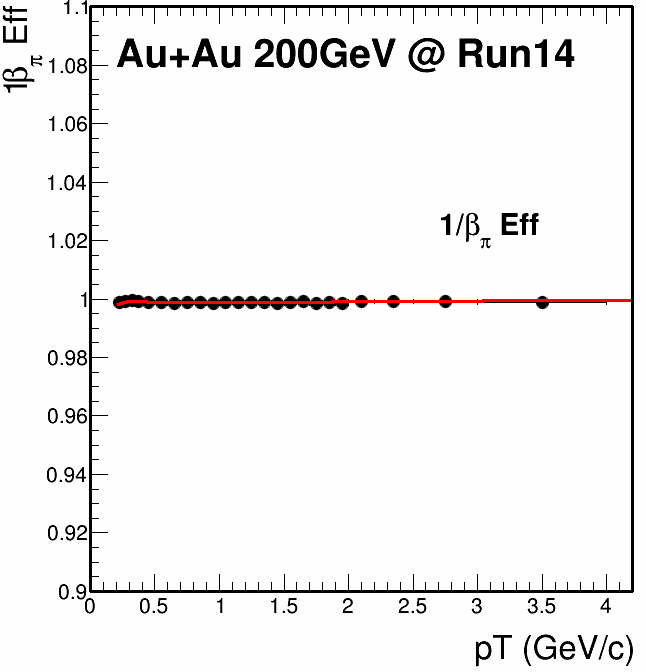
\includegraphics[width=1.0\textwidth]{fig/nSigPionTof_eff.png}
\caption{$1/\beta$ cut efficiency along with momentum for pion. Red line is the fitted function. \label{fig:piontofeff}}
\end{minipage}
\hfill
\begin{minipage}[htbp]{0.5\linewidth}
\centering
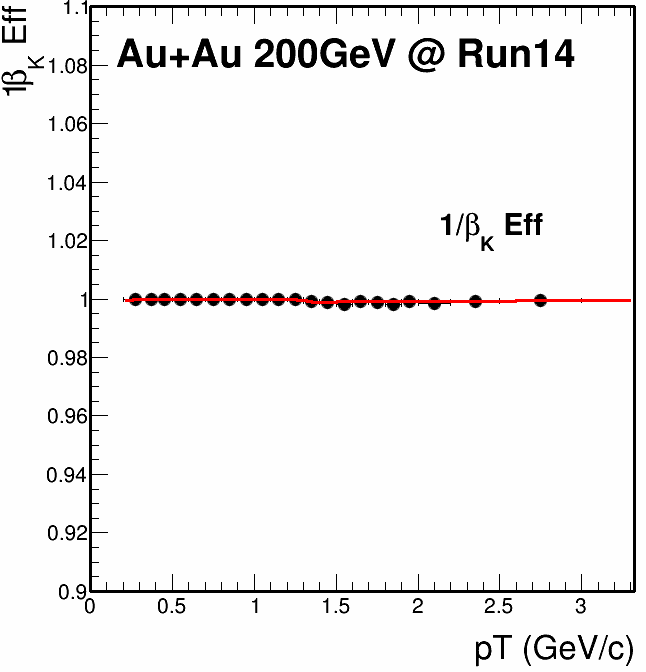
\includegraphics[width=1.0\textwidth]{fig/nSigKaonTof_eff.png}
\caption{$1/\beta$ cut efficiency along with momentum for kaon. Red line is the fitted function. \label{fig:kaontofeff}}
\end{minipage}
\end{figure}


\subsection{Data-driven fast Monte Carlo setup for HFT and Topological Cut Efficiency}

As discussed in the beginning of this section, the HFT related efficiency shown on Eq.~\ref{effEqu} including two items: HFT acceptance and topological cuts. Since the HFT embedding is not ready yet at that time, we developed the `Data-Driven Fast simulation' for the HFT related efficiency correction. And this method was validated with full GEANT simulation and will be discuss later.

\subsubsection{Assumptions}
\label{assumptions}
Before we discuss the details procedure of the method, it's better to make it clear, this data-driven simulation is based on several assumptions. And the validating will be tested step by step in the later section.
\begin{itemize}
\item Factorization of tracking efficiency:
\begin{equation}
\frac{\textup{HFT}}{\textup{MC}} = \frac{\textup{HFT}}{\textup{TPC}} \times \frac{\textup{TPC}}{\textup{MC}}
\label{efffact}
\end{equation}
\item Spatial resolution of HFT is encoded in two variables: $\textup{DCA}_{\textup{XY}}$ and $\textup{DCA}_{\textup{Z}}$ (two dimensions correlated).
\item Vertex resolution, which is possibly folded in the DCA resolution of single tracks and correlated for kaons and pions, is a negligible, at least for semi-central to central events.
\item The contribution of feed-down particles from secondary decays to DCA distributions is negligible.
\item Mis-matched daughter tracks are removed by topological cuts.
\end{itemize}

\subsubsection{Ingredients}
\label{ingredients}
There are several input ingredients for this fast-simulation package which is extracted from data.
\begin{itemize}
\item Extract $\textup{V}_\textup{z}$ distributions from data (centrality dependent).
\item Extract ratio of HFT matched tracks to TPC tracks from data (This ratio includes all mismatched tracks) (particle species, centrality, $p_T$, $\eta$, $\phi$, $\textup{V}_\textup{z}$ dependence).
\item Extract $\textup{DCA}_{\textup{XY}}$ - $\textup{DCA}_{\textup{Z}}$ distributions from data. Assuming that data DCA distributions is dominated by primary particles (particle species, centrality, $p_T$, $\eta$, $\textup{V}_\textup{z}$ dependence).
\item Extract TPC efficiency and momentum resolution from embedding (particles, centrality and $p_T$ dependence).
\end{itemize}

Fig.~\ref{hftRatioExample} shows an example of the input HFT match ratio in the certain $\eta$, $\textup{V}_\textup{Z}$, $\phi$ and centrality range. The HFT match ratio increase in the low pt range due to the high mismatch occupancy and keep flat in the high $p_T$ range. This ratio have a strong dependence on these differential such as $\eta$ and $\textup{V}_\textup{Z}$ since this is effected by HFT acceptance. Fig.~\ref{DcaExample} shows an example of the $\textup{Dca}_{\textup{XY}}$ vs $\textup{Dca}_{\textup{Z}}$ distribution in the certain $p_T$, $\eta$, $\textup{V}_\textup{Z}$ and centrality range. The axis binning is dynamic binning (non-uniform) since the most central (around 0) part is the dominate part. Limited by the computing memory, the most central part use fine binning and others use the unrefined binning as shown on the plots.

In total, there are 11 ($\phi$) $\times$ 10 ($\eta$) $\times$ 6 ($\textup{V}_\textup{z}$) $\times$ 9 (centrality) $\times$ 2 (particles) 1D histograms (36 $p_T$ binning) for HFT match efficiency.
There are 5 ($\eta$) $\times$ 4 ($\textup{V}_\textup{z}$) $\times$ 9 (centrality) $\times$ 2 (particles) histograms $\times$ 19 ($p_T$) 2D histograms (144 $\times$ 144 Dca binning) for Dca resolution smearing.

Effectively, these 1D and 2D histograms encode HFT efficiency, acceptance and spatial resolution performance in Run14 data.

\begin{figure}[htbp]
\begin{minipage}[htbp]{0.52\linewidth}
\centering
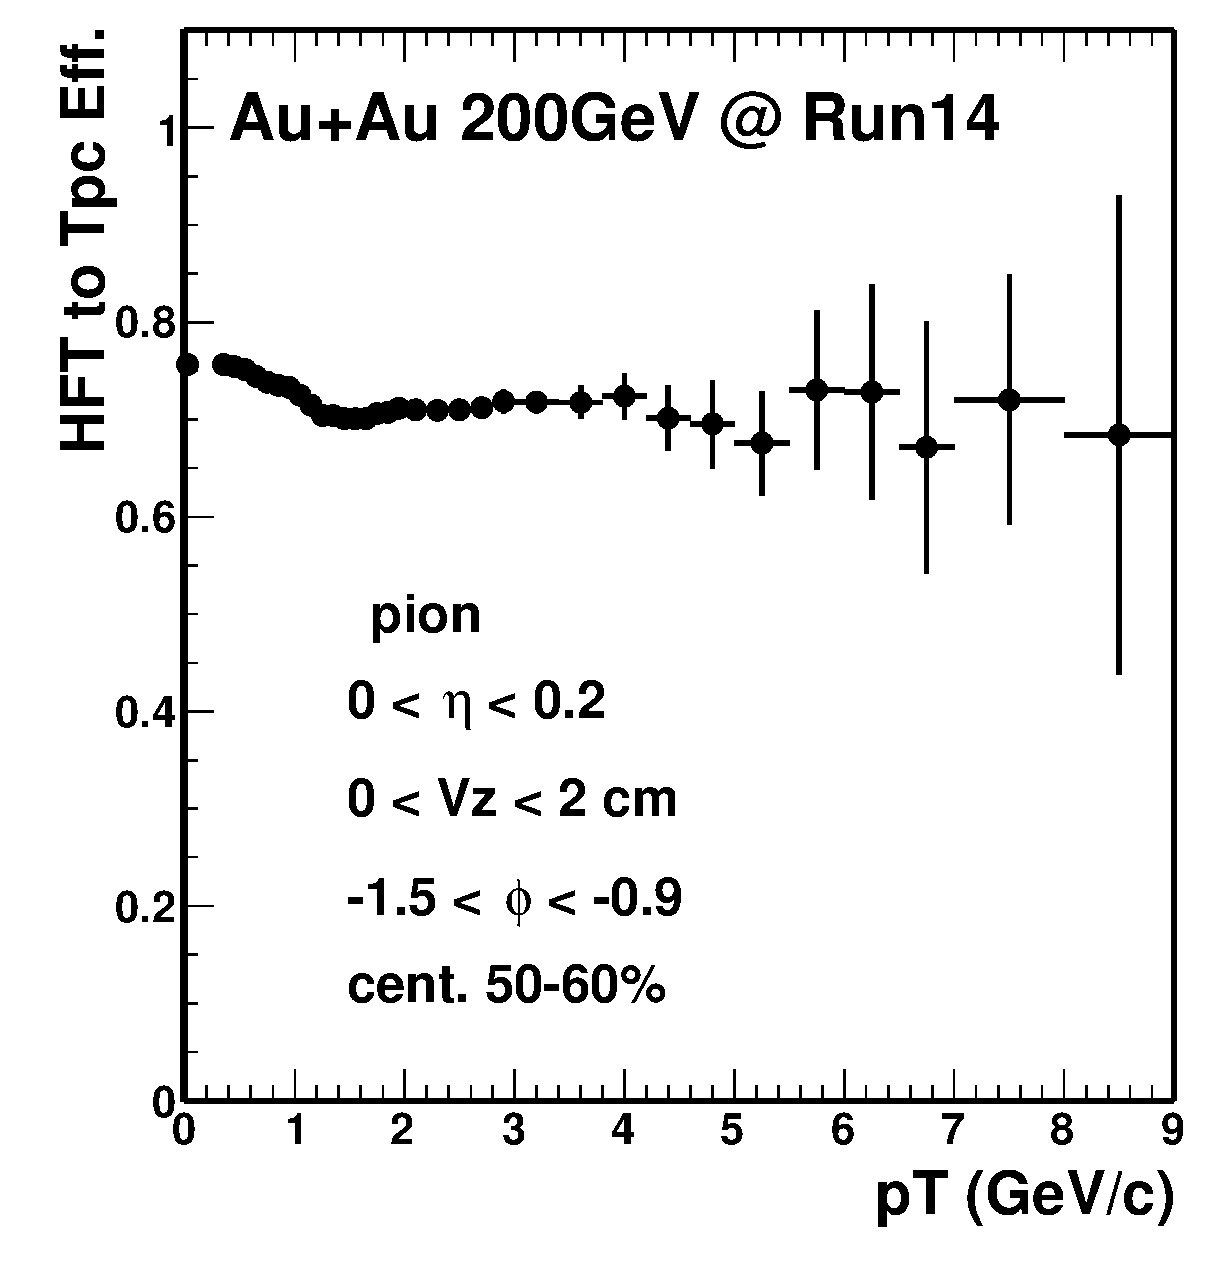
\includegraphics[width=1.0\textwidth,angle=0]{fig/hftRatioExample.eps}
\caption{ HFT to TPC track match ratio for pion at certain $\eta$,$\textup{V}_{\textup{Z}}$,$\phi$,centrality range. \label{hftRatioExample}}
\end{minipage}
\hfill
\begin{minipage}[htbp]{0.52\linewidth}
\centering
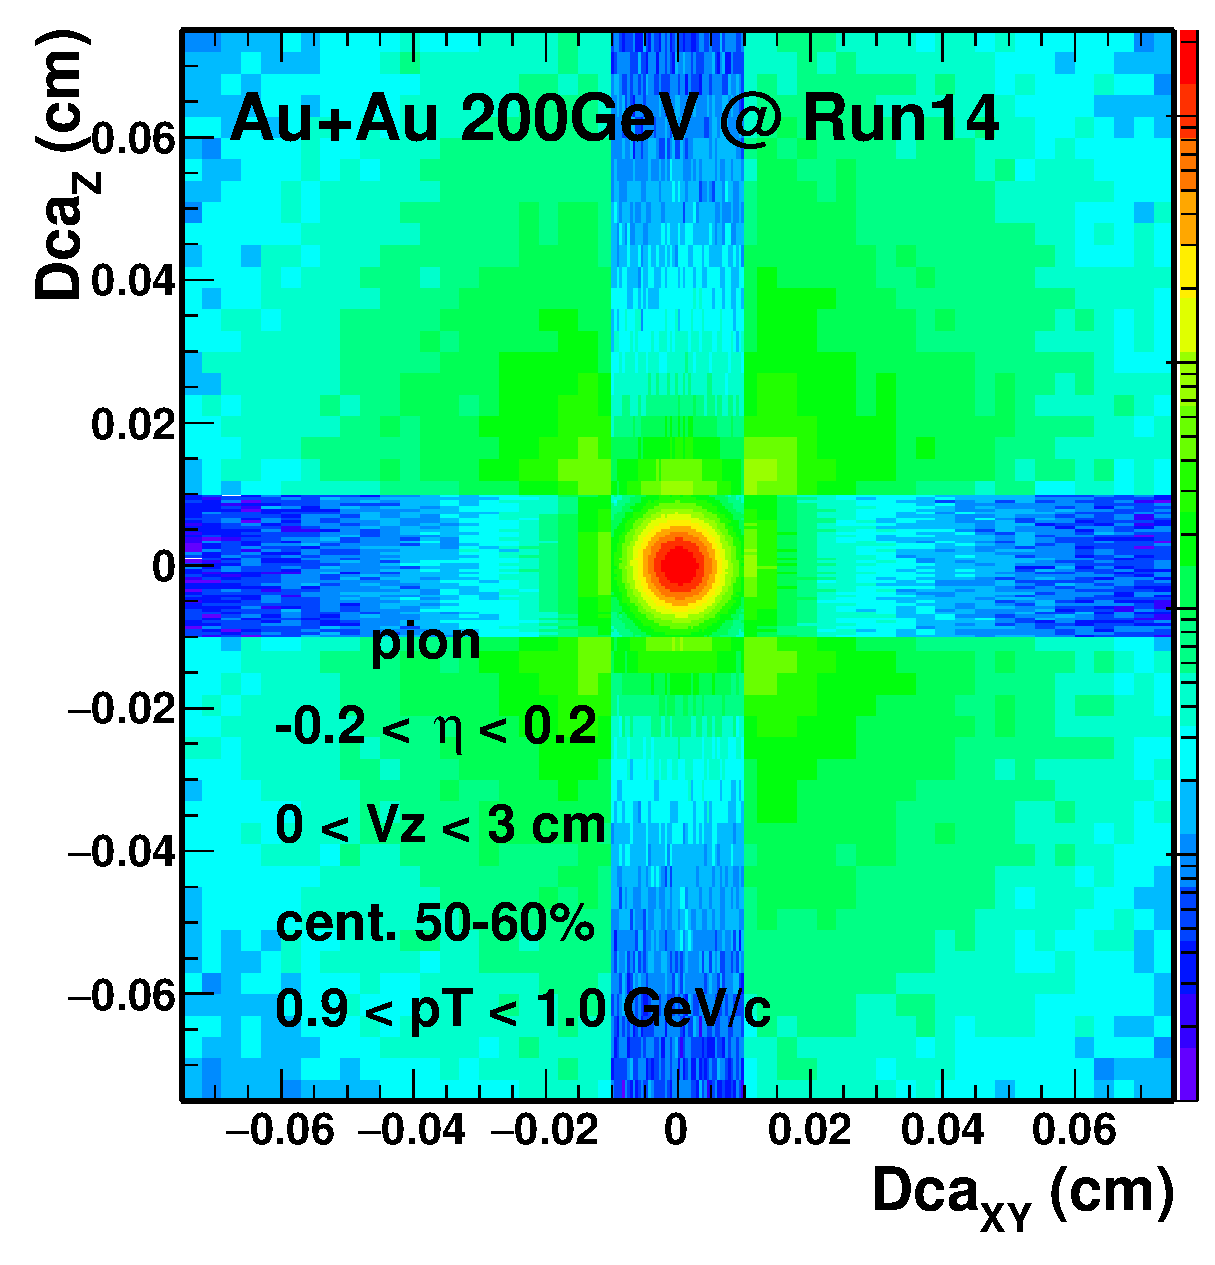
\includegraphics[width=1.0\textwidth,angle=0]{fig/DcaExample.eps} 
\caption{$\textup{Dca}_{\textup{XY}}$ vs. $\textup{Dca}_\textup{Z}$ for pion at certain $\eta$,$\textup{V}_{\textup{Z}}$,centrality range. \label{DcaExample}}
\end{minipage}
\end{figure}

\subsubsection{Recipe}
\label{recipe}
After all the input ingredients ready for the fast-simulation, a simple toy MC simulation (PYTHIA/EvtGen) is applied for the efficiency study. The basic recipe is following:
\begin{itemize}
\item Sample $\textup{V}_\textup{z}$ distribution according to data distribution.
\item Generate $D^0$ flat in $p_T$ and rapidity and decay it.
\item Smear momentum according the embedding.
\item Smear $DCA_{\textup{XY}}$ and $DCA_\textup{Z}$ of Kaons and Pions independently according to distributions from data.
\item Apply HFT matching efficiency from HFT ratio.
\item Apply TPC reconstruction efficiency.
\item Reconstruct $D^0$
\end{itemize}

\subsubsection{$D^0$ Efficiency and Topological Distribution}

As discussed in the recipe, we obtain the efficiency step by step as shown on Fig.~\ref{D0effStep}. First we have the TPC efficiency shown by red maker which is after the $p_T$, $\eta$ acceptance cut and TPC tracking efficiency from embedding. Then after folding in the HFT matching efficiency, the second item is obtained on black circle. Last step is after the topological cut, as shown by the cyan marker. As see in the low $p_T$ part, the topological cut efficiency is really small due to the tight cut as the combinatorial background is huge.

\begin{figure}[htbp]
\begin{minipage}[htbp]{0.52\linewidth}
\centering
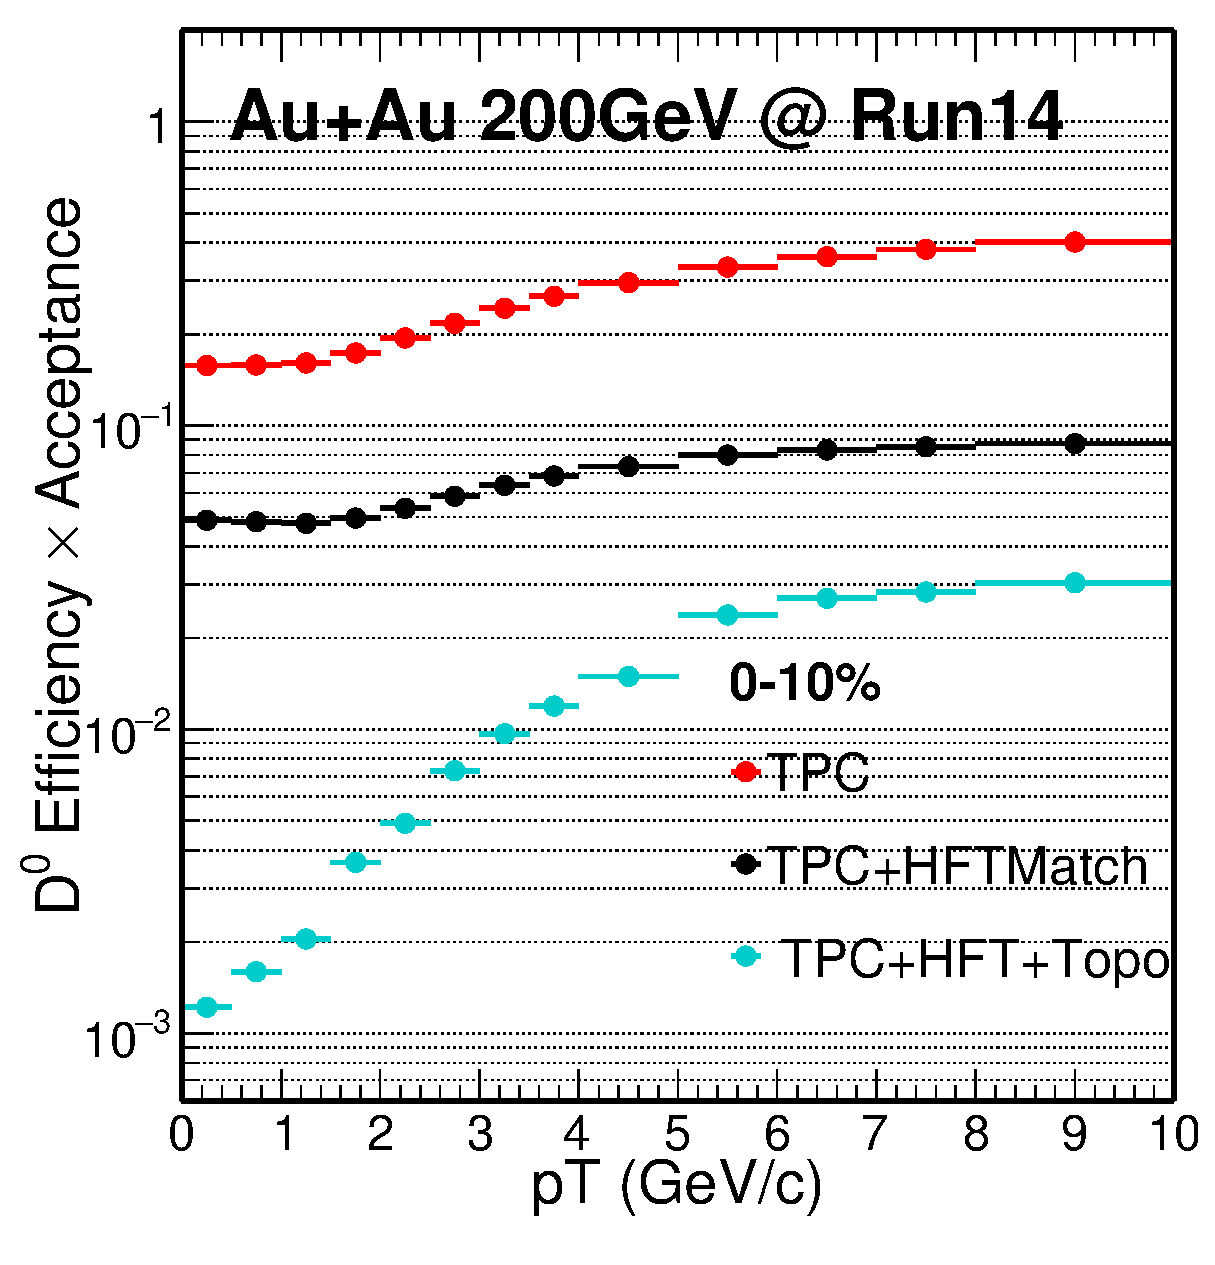
\includegraphics[width=1.0\textwidth,angle=0]{fig/HFT_efficiencyCombineStepbyStep_2.eps}
\caption{ $D^0$ efficiency step by step from TPC, HFT Ratio, Topological cut in most central 0-10\%. \label{D0effStep}}
\end{minipage}
\hfill
\begin{minipage}[htbp]{0.52\linewidth}
\centering
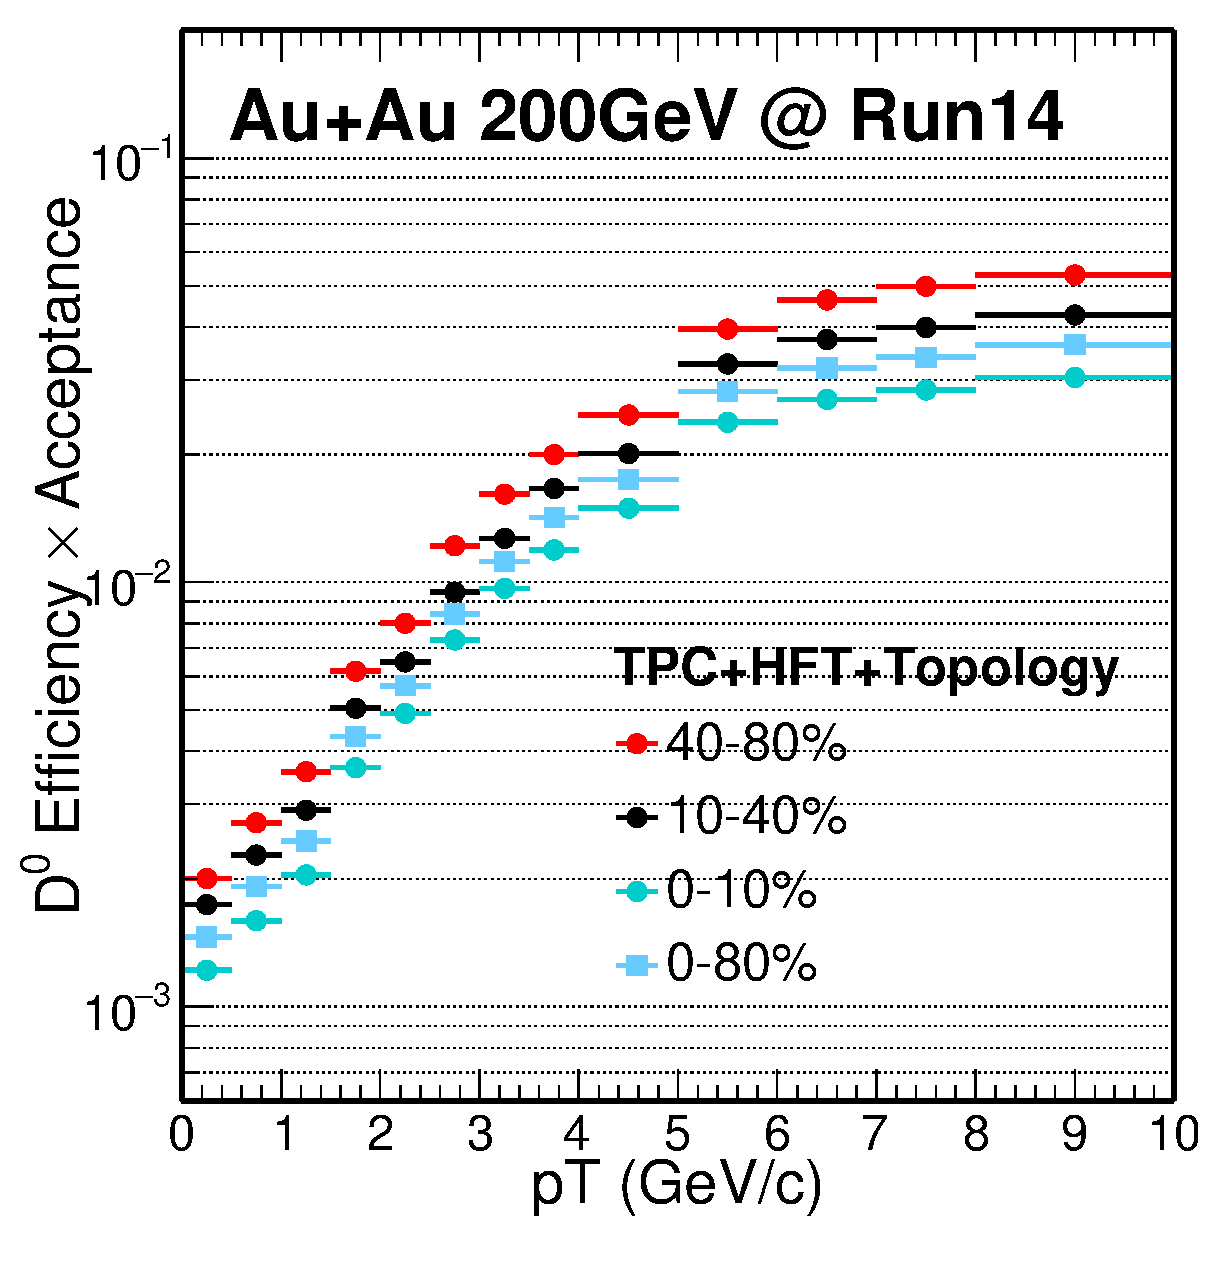
\includegraphics[width=1.0\textwidth,angle=0]{fig/HFT_efficiencyCombineCompare_5.eps} 
\caption{ $D^0$ efficiency including TPC, HFT and Topological cut in several centralities. \label{D0effCombine}}
\end{minipage}
\end{figure}

We study all the efficiencies with small centrality bin width, in total we have 9 centrality bins from our StRefmultCorr class. Since the $D^0$ production is scaled by the number of binary collisions ($\textup{N}_{\textup{bin}}$), the $D^0$ is favor produced in more central collisions. So the final efficiencies for the wider centrality bins 0-10\%, 10-40\%, 40-80\% and 0-80\% are calculated using $\textup{N}_{\textup{bin}}$ as weights, for example, the efficiency in 0-80\% is calculated as the following Eq.~\ref{effcombine}. Fig~\ref{D0effCombine} shows the $D^0$ efficiency for 4 wide centralities after TPC, HFT match and Topological efficiency included.

\begin{equation}
  \textup{Efficiency}_{0-80\%} = \sum_{i=1}^{9}(\textup{Efficiency}_{i} \times N_{bin}^{i}) / <\textup{N}_{\textup{bin}}>
\label{effcombine}
\end{equation}

The Data-Driven Fast-Simulation also provide the topological information, can be used for the comparison with real data. For the real data part, within the $D^0$ mass window we can statistical subtract the background and extract the pure $D^0$ topological distributions. The invariant mass plots shown as Fig.~\ref{d0massforTopo}. $D^0$ is in the 2 < $p_T$ < 3 GeV/$c$, 0-80\% centrality. Black is unlikesign foreground, blue is likesign background and red is mixed event background. The blue vertical lines are the mass window used for the topological comparison. For each topological variable, that corresponding topological cut was removed when reconstruct the $D^0$ candidate, so that we can compare that variable in a wide range.

\begin{figure}[htbp]
\centering
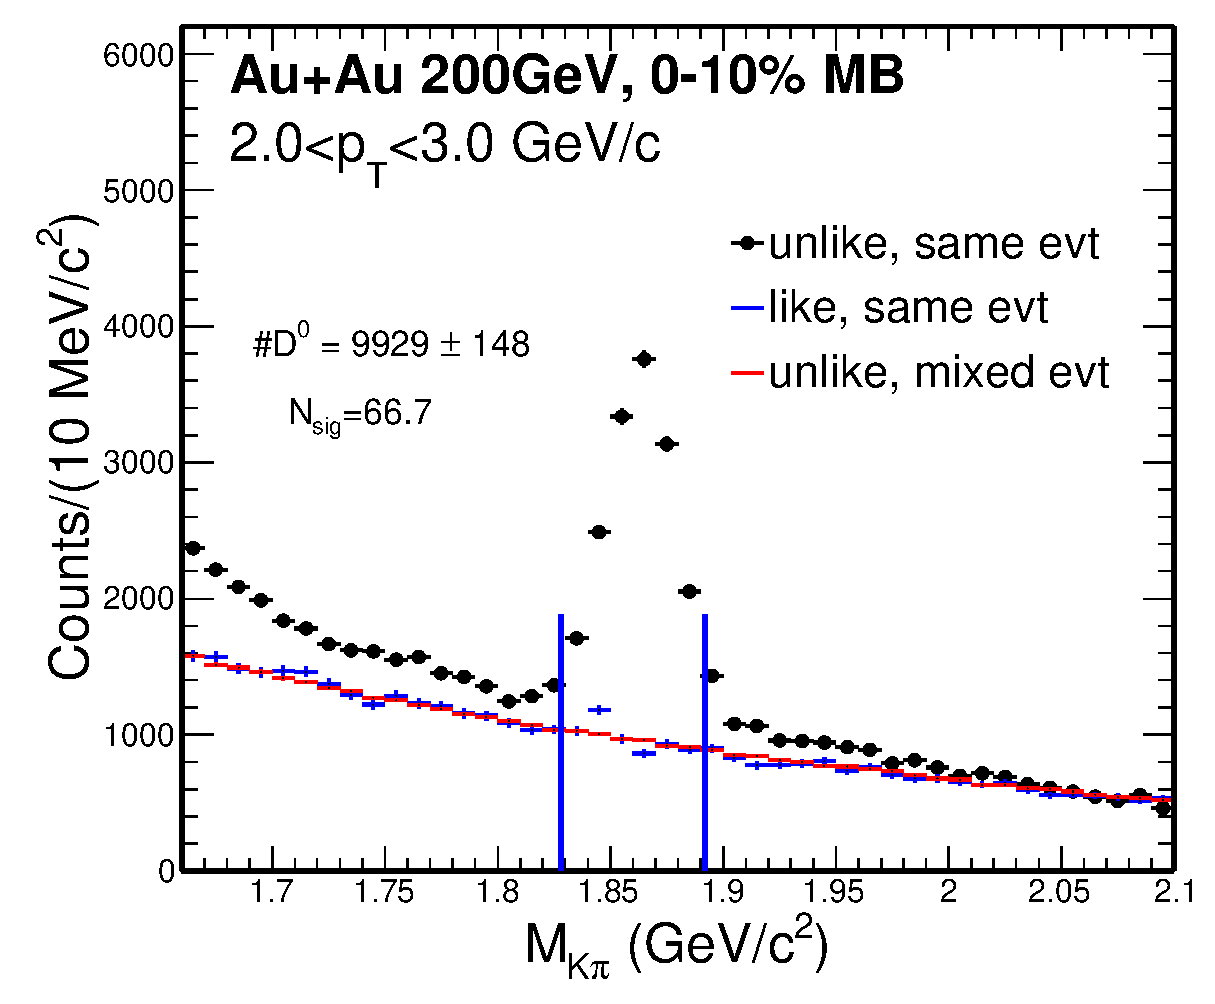
\includegraphics[keepaspectratio,width=0.6\textwidth]{fig/Mixed_cent_8_9_pt_2_3.eps}
\caption{$D^0$ invariant mass distributions in the 2 < $p_T$ < 3 GeV/$c$, 0-10\% centrality. Black is unlikesign foreground, blue is likesign background and red is mixed event background. The blue vertical lines are the mass window used for the topological comparison.}
\label{d0massforTopo}
\end{figure}

\begin{figure}[htbp]
\begin{minipage}[htbp]{0.52\linewidth}
\centering
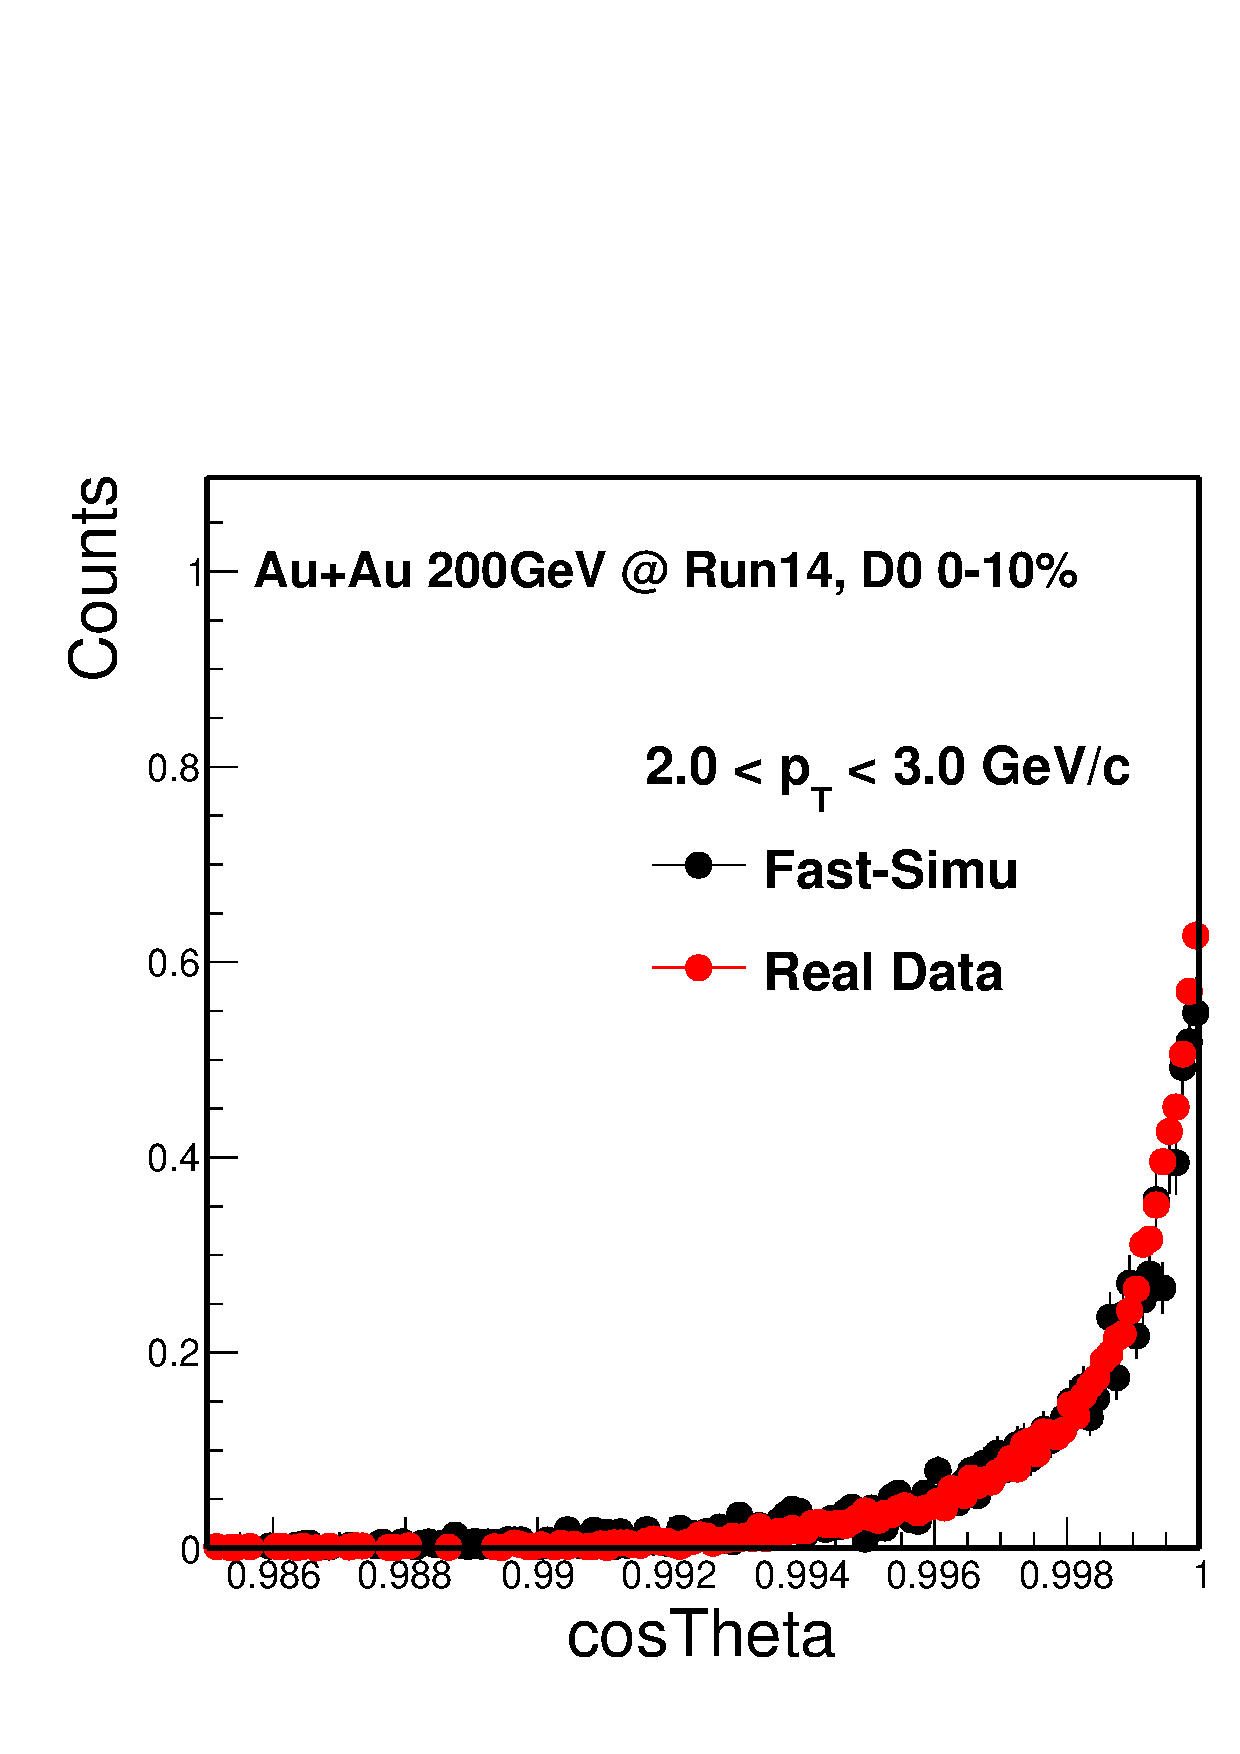
\includegraphics[width=1.0\textwidth,angle=0]{fig/pointingangle.pdf}
\caption{ $D^0$ cosTheta distribution in most central 0-10\% between Fast-Simulation and Real Data.\label{pointingangle}}
\end{minipage}
\hfill
\begin{minipage}[htbp]{0.52\linewidth}
\centering
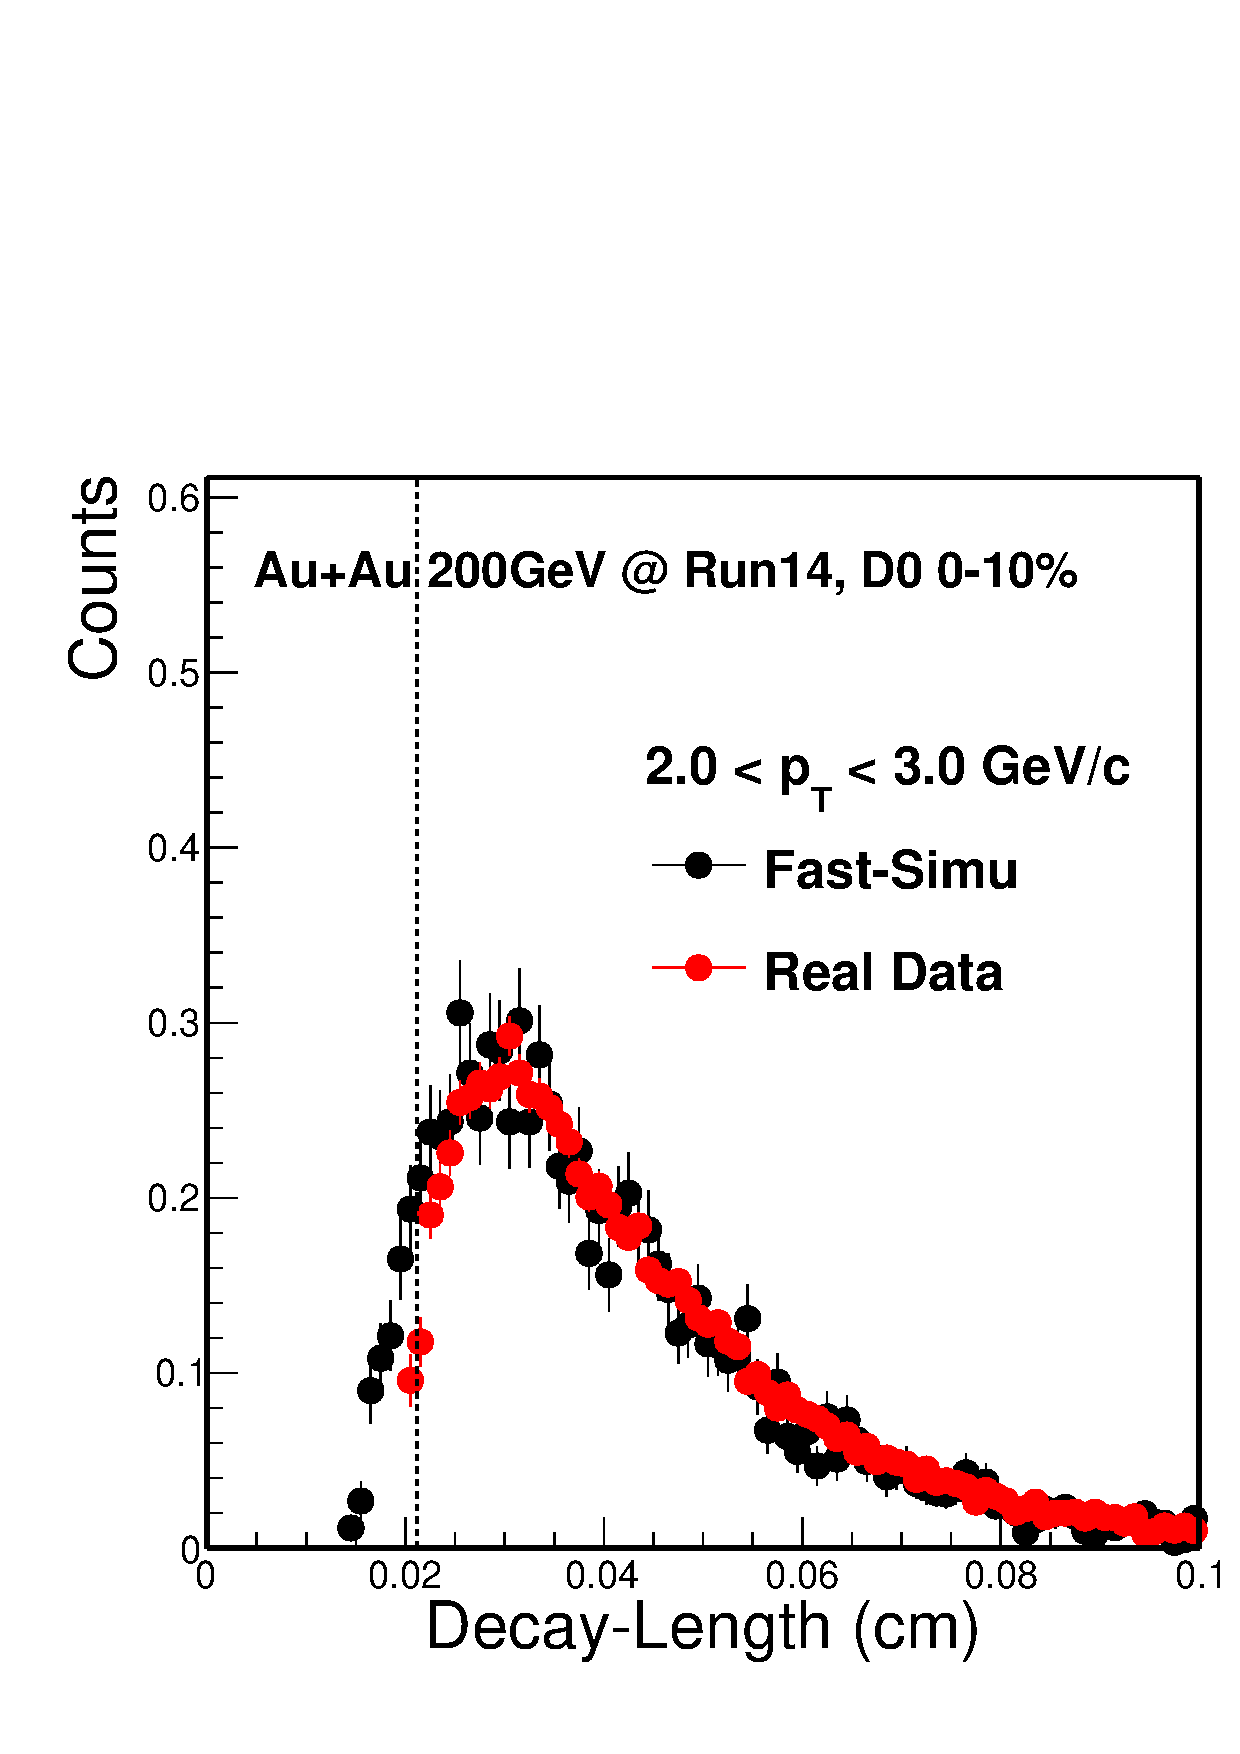
\includegraphics[width=1.0\textwidth,angle=0]{fig/DecayL.pdf} 
\caption{ $D^0$ decay length distribution in most central 0-10\% between Fast-Simulation and Real Data.\label{DecayL}}
\end{minipage}
\end{figure}

\begin{figure}[htbp]
\begin{minipage}[htbp]{0.52\linewidth}
\centering
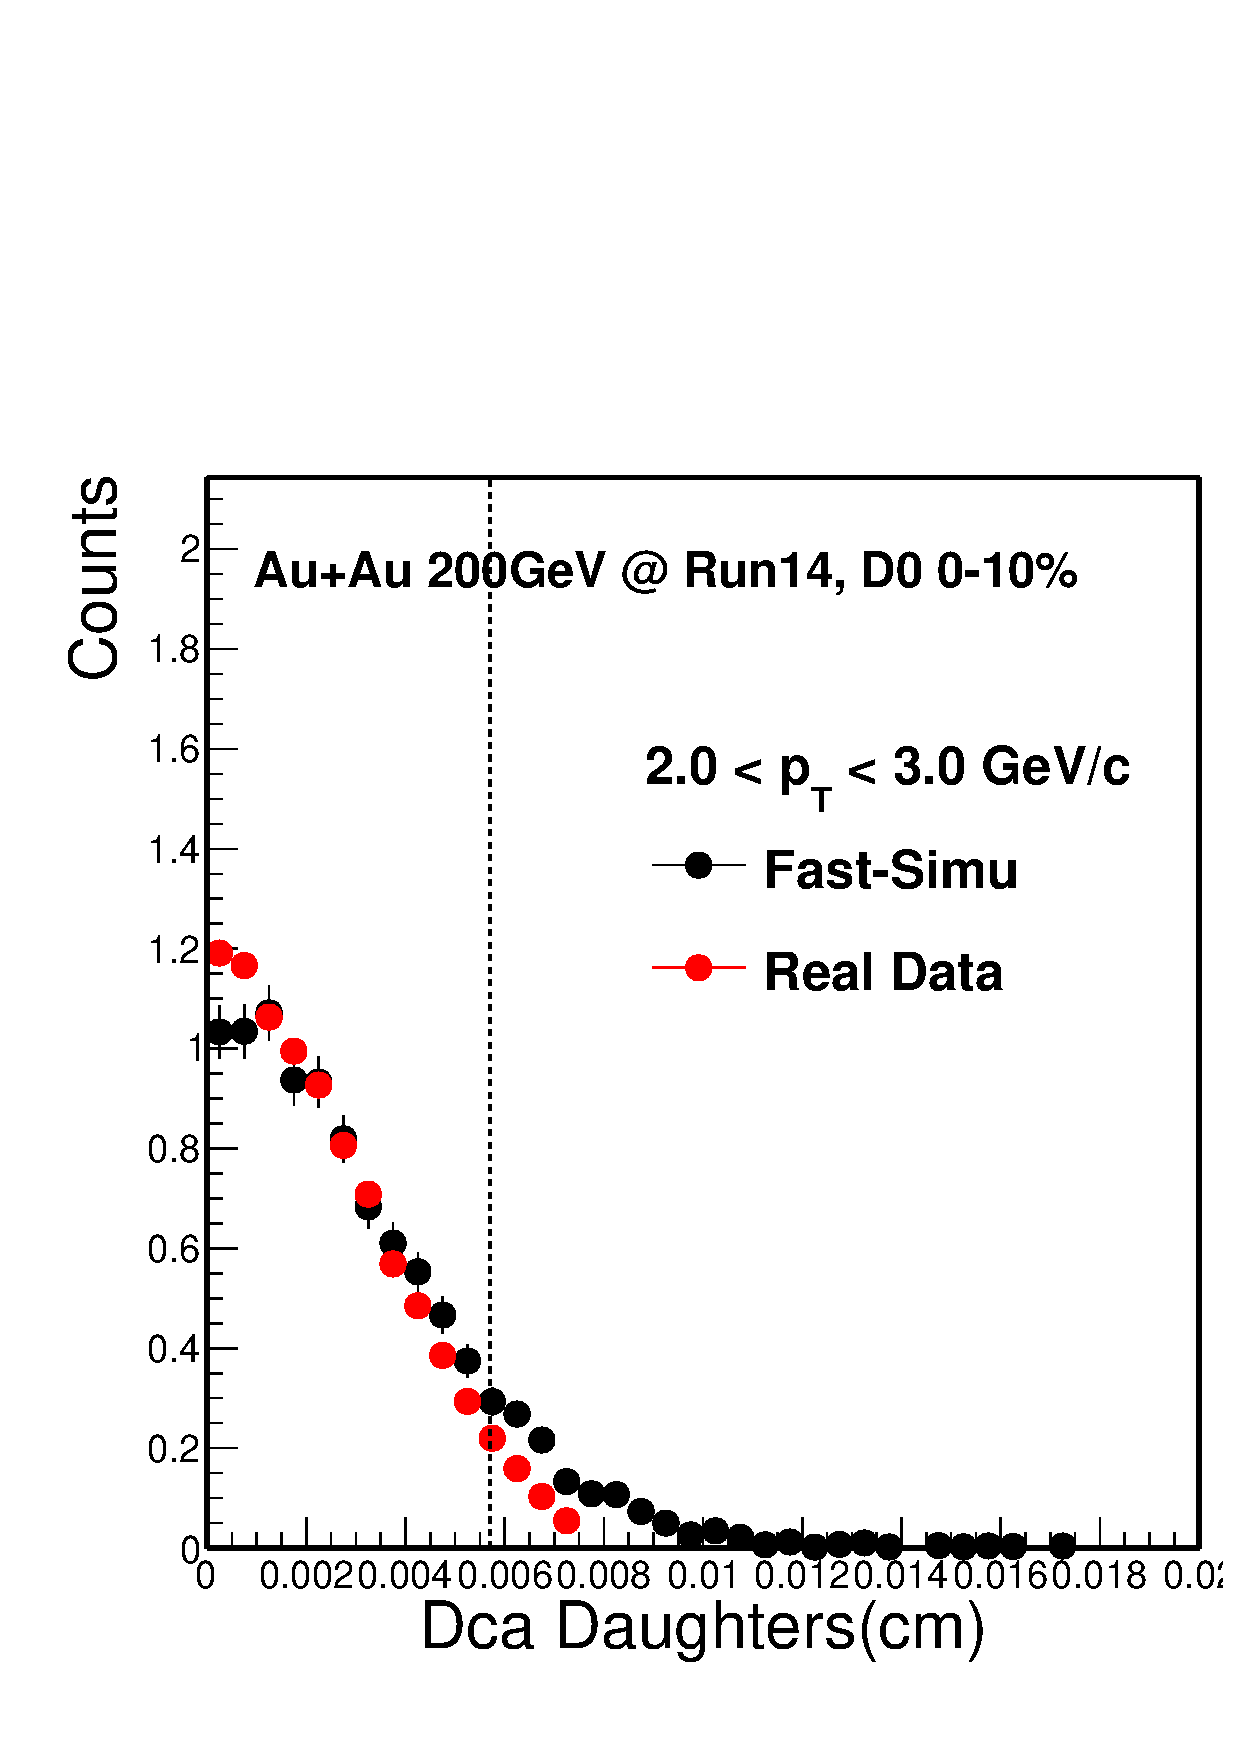
\includegraphics[width=1.0\textwidth,angle=0]{fig/dcaDaughters.pdf}
\caption{ $D^0$ dcaDaughters distribution in most central 0-10\% between Fast-Simulation and Real Data.\label{dcaDaughters}}
\end{minipage}
\hfill
\begin{minipage}[htbp]{0.52\linewidth}
\centering
\includegraphics[width=1.0\textwidth,angle=0]{fig/D0Dca2Vtx.pdf} 
\caption{ $D^0$ dca to Vertex distribution in most central 0-10\% between Fast-Simulation and Real Data.\label{D0Dca2Vtx}}
\end{minipage}
\end{figure}

\begin{figure}[htbp]
\begin{minipage}[htbp]{0.52\linewidth}
\centering
\includegraphics[width=1.0\textwidth,angle=0]{fig/pionDca.pdf}
\caption{ $D^0$ pionDca distribution in most central 0-10\% between Fast-Simulation and Real Data. \label{pionDca}}
\end{minipage}
\hfill
\begin{minipage}[htbp]{0.52\linewidth}
\centering
\includegraphics[width=1.0\textwidth,angle=0]{fig/kaonDca.pdf} 
\caption{ $D^0$ kaonDca distribution in most central 0-10\% between Fast-Simulation and Real Data. \label{kaonDca}}
\end{minipage}
\end{figure}

From Fig.~\ref{pointingangle} to Fig.~\ref{kaonDca}, these are the topological variables (cos($\theta$), decayLength, dcaDaughters, D0DcaToVtx, PionDca and KaonDca) used for the $D^0$ reconstruction. The distributions from the real data part are using mixed event method to statistical subtract the background. The Data-Driven Fast-Simulation part was the package we relayed on for our efficiency study as shown before.

Comparison these topological variables between real data and Fast-Simulation, the agreement is reasonable good, which means our Data-Driven Fast-Simulation method can well reproduce the topological variables in real data. In another word, the efficiency estimation from Data-Driven Fast-Simulation is reliable. Note, there are some small discrepancy such as single track Dca distributions in the low end, that's because in the data analysis part, we already require some minimum cut in order to save the computing resource. There is another method we are going to discuss in the following section, also can be used to validating our Fast-Simulation method.

\subsection{Validation with Full GEANT+Hijing Simulation}

Before discuss the details of this Hijing validation, it's better to conclude those assumptions we made before. The first assumption is the factorization shown in Eq.~\ref{efffact}. Relaying on the Hijing simulation, we have two samples. One is only include TPC tracking, another one include both HFT and TPC in tracking. From the first sample, we can extract the TPC factorized tracking efficiency, and the second sample can be used to extract the overall total efficiency and HFT over TPC factorized efficiency separately. Fig.~\ref{assumption01} shows the comparison between the overall efficiency and the multiplied factorization efficiency. The red one is from overall efficiency from the second sample, and the blue one is multiplied efficiency from two components. The bottom panel shows the double ratio of these two efficiency, and they are perfectly factorized as the ratio is flat as unity.

\begin{figure}[htbp]
\centering
\includegraphics[keepaspectratio,width=0.7\textwidth]{fig/assumption01.png}
\caption{(top)HFT Efficiency Factorization comparison. (bottom) Double Ratio of these factorization.}
\label{assumption01}
\end{figure}

The second assumption is for the spatial resolution, it is encoded in those $\textup{Dca}_{\textup{XY}}$ and $\textup{Dca}_{\textup{Z}}$ variables, and they are correlated in the two dimensions. Fig.~\ref{assumption2} shows the comparison between the input Dca from real data and output Dca from Fast-Simulation in three dimensions. The first row is Dca in XY plane, the second row is in Z plane and the last row is in the 3-D dimension. From the left to right is the comparison from low $p_{T}$ to high $p_{T}$. As shown the red line is from data and black line is from fast simulation, the agreement is pretty good.
For the others assumption, they will be discussed separately in the following section.

\begin{figure}[htbp]
\centering
\includegraphics[keepaspectratio,width=1.0\textwidth]{fig/assumption2.png}
\caption{Comparison of Dca between data (red) and Fast-Simulation (black). From top to bottom, the comparison is for $\textup{Dca}_{\textup{XY}}$, $\textup{Dca}_{\textup{Z}}$ and $\textup{Dca}$. From left to right the transverse momentum is from low $p_T$ to high $p_T$.}
\label{assumption2}
\end{figure}

\subsection{Hijing Samples Performance}
\label{hijingsample}
The Hijing sample was run through the Full Hijing + GEANT simulation with realistic pileup hits (UPC+MB) in PXL and sensor masking tables. They can provide reasonable performance for the HFT matching ratio and Dca resolution. 
In total we have $\sim$45K 0-10\% centrality Hijing events, and for each event is embedded with 20 $D^0$'s. So in total, we have $\sim$900K $D^0$ for this Hijing sample. The embedded $D^0$ has small effect on the tracking since the multiplicity is much higher compared to 20 $\times$ 2 $D^0$' decayed daughters.

\begin{figure}[htbp]
\begin{minipage}[htbp]{0.52\linewidth}
\centering
\includegraphics[width=1.0\textwidth,angle=0]{fig/HijingRatio.eps}
\caption{ HFT Ratio comparison between data and Hijing simulation in Au+Au 200 GeV/c, 0-10\%.\label{HijingRatio}}
\end{minipage}
\hfill
\begin{minipage}[htbp]{0.52\linewidth}
\centering
\includegraphics[width=1.0\textwidth,angle=0]{fig/HijingDca.eps} 
\caption{ $\pi^{\pm}$ $\textup{Dca}_{\textup{XY}}$ comparison between data and Hijing simulation in Au+Au 200 GeV/c, 0-10\%.\label{HijingDca}}
\end{minipage}
\end{figure}

As shown in Fig.~\ref{HijingRatio} is the HFT matching ratio comparison between data (red) and Hijing samples (black) in Au+Au 200 GeV/$c$ from 0-10\% centrality, the bottom panel is the double ratio of these two HFT matching ratio. The value is around unity, which means the Hijng simulation can well reproduce these matching performance. 

Fig.~\ref{HijingDca} shows the pions $\textup{Dca}_{\textup{XY}}$ comparison between data (red) and Hijing samples (black) in Au+Au 200 GeV/$c$ from 0-10\% centrality at 1.0 < $p_T$ < 1.2GeV/$c$, the bottom panel is the double ratio of these two Dca distributions. The value is also around unity, which means the Hijng simulation well describes the real data.

\subsection{Validation Procedures}
\label{validationprocedure}

The idea is simple for this Hijing validation, we have the enriched $D^0$ Hijing sample. After run through the detector and full GEANT simulation, the $D^0$ efficiency and topological variables distributions can be extracted. Another procedure is extract the necessary ingredients from Hijng sample for the Fast-Simulation input (Fast-Simulation with Hijing input), such as the TPC Tracking efficiency, the HFT matching ratio and the 2D $\textup{Dca}_\textup{XY}$-$\textup{Dca}_\textup{Z}$ distributions similar as we used in real data analysis and discussed in the previous section. Then run through the Fast Simulation, as discussed before, the $D^0$ efficiency and topological variables are also available in this way and can be compared to the first Hijing + GEANT procedure. The workflow is shown in Fig.~\ref{validation0}.

\begin{figure}[htbp]
\centering
\includegraphics[keepaspectratio,width=1.0\textwidth]{fig/validation0.pdf}
\caption{Hjiing validation procedure and workflow}
\label{validation0}
\end{figure}

\subsubsection{Validation Efficiency}
\label{validationeff}

The first step is to check the kinematic form different MC decayer such as PYTHIA, Hijing, evtGen and PhaseSpace class from ROOT. Need to make sure the decayer used for Fast-Simulation has the same kinematic as the Hijng. After the basic acceptance cut, such as $D^0$ |y| < 1, daughter $p_T$ > 0.2 GeV/$c$ and |$\eta$| <1 cut. $D^0$ is the simple phase space decay, all these decayer give the same acceptance efficiency as shown in Fig.~\ref{d0decayer} left panel, the right panel shows the double ratio to PYTHIA. As all the decayer follow the same trend they have the same decay kinematic, so, for our Fast-Simulation decayer we choose PYTHIA for this validation and also for our real data analysis.

\begin{figure}[htbp]
\centering
\includegraphics[keepaspectratio,width=1.0\textwidth]{fig/Acceptance_D0Decayer.eps}
\caption{$D^0$ pure acceptance from different MC decayer, such as PYTHIA, Hijing, evtGen and PhaseSpace class. (right) Double ratio of the acceptance to PYTHIA.}
\label{d0decayer}
\end{figure}

The second step is to check the kinematic with the reconstructed TPC tracking information. Compare to the first step, this one fold in the momentum resolution and the TPC acceptance effect. Fig.~\ref{d0tpceff} left panel shows this efficiency $\times$ Acceptance comparison between Hijing + GEANT (red) and Fast-Simulation with Hijing input (black), the right panel shows the double ratio to Hijing. As the red line is the fit function and the fit results around $\sim$1 shows very good agreement, which means this step is also doing right work.

\begin{figure}[htbp]
\centering
\includegraphics[keepaspectratio,width=1.0\textwidth]{fig/Physics_FastHijingVsPureHijing_TpcOnly2.eps}
\caption{The comparison of $D^0$ TPC acceptance $\times$ efficiency between Hijing + GEANT (red) and Fast-Simulation with Hijing input (black). (right) Double ratio of these acceptance to Hijing.}
\label{d0tpceff}
\end{figure}

The next step is to trying to fold in the HFT matching efficiency and this is to consider the HFT acceptance effect. Fig.~\ref{d0hftmatcheff} left panel shows this efficiency $\times$ Acceptance comparison after TPC and HFT matching between Hijing + GEANT (red) and Fast-Simulation (black), the right panel shows the double ratio to Hijing. As the red line is the fit function and the fit results around $\sim$1 shows good agreement, which means this HFT matching step is also correctly implemented in the package. For the small discrepancy at the high $p_T$ range, this is purely due to the limited statistics. Since the Hijing sample is time consumption, we do not have enough statistics for the HFT match ratio input. But this problem is not exist for our real data analysis since we have $\sim$900M events which is totally enough and we checked the HFT match ratio, they can extend to a reasonable high $p_T$ range in real data. We did another small check, use one quart of these Hijing statistics for this validation, and the discrepancy shown here is bigger than the current results, which is another approve of the limited Hijing statistics.

\begin{figure}[htbp]
\centering
\includegraphics[keepaspectratio,width=1.0\textwidth]{fig/Physics_FastHijingVsPureHijing_HFTRatio2.eps}
\caption{The comparison of $D^0$ TPC + HFT match acceptance $\times$ efficiency between Hijing + GEANT (red) and Fast-Simulation with Hijing input (black). (right) Double ratio of these acceptance to Hijing.}
\label{d0hftmatcheff}
\end{figure}

The last step is folding in the topological cuts and then compare between the Hijing and Fast-Simulation. Fig.~\ref{d0hfttopoeff} left panel shows this efficiency $\times$ Acceptance comparison after TPC, HFT matching and topological cuts between Hijing + GEANT (red) and Fast-Simulation (black), the right panel shows the double ratio to Hijing. Still the red line is the fit function and the fit results around $\sim$0.93 shows good agreement, which means this topological variables are well described in the package. For the left panel, there are some twist for this efficiency $\times$ acceptance at $p_T$ $\sim$1 GeV/$c$ and 2 GeV/$c$, this is due to the topological cuts are different in separate $p_T$ ranges. As the red points show the efficiency from Hijing + GEANT, the statistics error is larger compared to the Fast-Simulation which shows by black. This is also the reason we use data-driven Fast-Simulation for our efficiency study, it can be easily enlarge the statistics by a factor of 100 or even 1000 compare to the traditional Full GEANT simulation especially for this kind of low efficiency studies. Fig.~\ref{d0hfttopoeff2} shows the same plots of the comparison as Fig.~\ref{d0hfttopoeff} with different binning, we merged some binning for statistics concern. After merged the binning, the agreement is even better from the fitting shown on the right panel, the fitting results is $\sim$0.96.

\begin{figure}[htbp]
\centering
\includegraphics[keepaspectratio,width=1.0\textwidth,angle=0]{fig/Physics_FastHijingVsPureHijing_HFTTopo2.eps}
\caption{The comparison of $D^0$ TPC + HFT match + Topological acceptance $\times$ efficiency between Hijing + GEANT (red) and Fast-Simulation with Hijing input (black). (right) Double ratio of these acceptance to Hijing.}
\label{d0hfttopoeff}
\end{figure}

\begin{figure}[htbp]
\centering
\includegraphics[keepaspectratio,width=1.0\textwidth,angle=0]{fig/Physics_FastHijingVsPureHijing_HFTTopo.eps}
\caption{The comparison of $D^0$ TPC + HFT match + Topological acceptance $\times$ efficiency between Hijing + GEANT (red) and Fast-Simulation with Hijing input with wide binning (black). (right) Double ratio of these acceptance to Hijing.}
\label{d0hfttopoeff2}
\end{figure}

From Hijing + GEANT simulation, we know exactly whether the HFT matched track is real match or mismatch, so we can determine the HFT real matched efficiency $\times$ acceptance for $D^0$ reconstruction from Hijing sample. Fig.~\ref{d0hfttoporealeff} shows these real matched efficiency $\times$ acceptance comparison between Hijng + GEANT and our previously Fast-Simulation. The right panel shows the double ratio of these efficiency and fitted with a line, the parameters shows $\sim$0.98 which means the (previous) Fast-Simulation can well reproduce the real HFT matched reconstruction efficiency. Fig.~\ref{d0hfttoporealeff2} shows the same plots of the comparison with different binning. 

\begin{figure}[htbp]
\centering
\includegraphics[keepaspectratio,width=1.0\textwidth,angle=0]{fig/Real_Physics_FastHijingVsPureHijing_HFTTopo2.eps}
\caption{The comparison of $D^0$ TPC + HFT Real match + Topological acceptance $\times$ efficiency between Hijing + GEANT (red) and Fast-Simulation with Hijing input (black). (right) Double ratio of these acceptance to Hijing.}
\label{d0hfttoporealeff}
\end{figure}

\begin{figure}[htbp]
\centering
\includegraphics[keepaspectratio,width=1.0\textwidth,angle=0]{fig/Real_Physics_FastHijingVsPureHijing_HFTTopo.eps}
\caption{The comparison of $D^0$ TPC + HFT Real match + Topological acceptance $\times$ efficiency between Hijing + GEANT (red) and Fast-Simulation with Hijing input with wide binning (black). (right) Double ratio of these acceptance to Hijing.}
\label{d0hfttoporealeff2}
\end{figure}

If we compare with the previous Hijing HFT matched efficiency (not necessary to be real matched), it also indicate that most of the Mis-matched daughter tracks are removed by topological cuts as we said in the assumptions. Fig.~\ref{d0hfttopoAlleff} shows the different components contributions directly from Hijing, the black one is HFT matched, red one requires all the daughter tracks are real matched and the blue one shows at least one of the daughter tracks are mis-matched. Right panel shows the relative fraction of the real match and mis-mismatch contribution. As see, most of the mis-matched tracks are removed, but still there are $\sim$5\% contribution from this study.

\begin{figure}[htbp]
\centering
\includegraphics[keepaspectratio,width=1.0\textwidth,angle=0]{fig/ALL_Physics_FastHijingVsPureHijing_HFTTopo.eps}
\caption{The comparison of $D^0$ TPC + HFT (real/mis) match + Topological acceptance $\times$ efficiency for Hijing + GEANT. (right) Double ratio of the components form Hijing.}
\label{d0hfttopoAlleff}
\end{figure}

Above all the discussions in this section ~\ref{validationeff}, we are confident that the Fast-Simulation method can well reproduce the acceptance and efficiency for this HFT related analysis. The precision as shown on Fig.~\ref{d0hfttopoeff2} is good enough for our efficiency study. For the missed-match check, there are $\sim$5\% contributions in the signals. And there is another approvement that will describe in the following section.

\subsubsection{Validation Topological Distributions}
\label{validationTopo}

As discussed before, we can extract the topological variables from both Hijing + GEANT and Fast-Simulation relay on those Hijing input. Similar as we did in Sec. ~\ref{d0efficiency}, we can compare the topological distributions from these two procedures. This will be another evidence that our Fast-Simulation can well reproduce the topological variables which is crucial for these kind of secondary vertex reconstruction analysis.

\begin{figure}[htbp]
\begin{minipage}[htbp]{0.52\linewidth}
\centering
\includegraphics[width=1.0\textwidth,angle=0]{fig/HijingcosTheta.eps}
\caption{ $D^0$ cosTheta distribution in most central 0-10\% between Hijing and Fast-Simulation.\label{Hijingpointingangle}}
\end{minipage}
\hfill
\begin{minipage}[htbp]{0.52\linewidth}
\centering
\includegraphics[width=1.0\textwidth,angle=0]{fig/HijingDecayL.eps} 
\caption{ $D^0$ decay length distribution in most central 0-10\% between Hijing and Fast-Simulation.\label{HijingDecayL}}
\end{minipage}
\end{figure}

\begin{figure}[htbp]
\begin{minipage}[htbp]{0.52\linewidth}
\centering
\includegraphics[width=1.0\textwidth,angle=0]{fig/HijingdcaPions.eps}
\caption{ $D^0$ pions Dca distribution in most central 0-10\% between Hijing and Fast-Simulation.\label{HijingdcaPions}}
\end{minipage}
\hfill
\begin{minipage}[htbp]{0.52\linewidth}
\centering
\includegraphics[width=1.0\textwidth,angle=0]{fig/HijingdcaKaons.eps} 
\caption{ $D^0$ kaons Dca distribution in most central 0-10\% between Hijing and Fast-Simulation.\label{HijingdcaKaons}}
\end{minipage}
\end{figure}

\begin{figure}[htbp]
\centering
\includegraphics[keepaspectratio,width=0.52\textwidth]{fig/HijingdcaDaughters.eps}
\caption{$D^0$ dcaDaughters distribution in most central 0-10\% between Hijing and Fast-Simulation.}
\label{HijingdcaDaughters}
\end{figure}

From Fig.~\ref{Hijingpointingangle} to Fig.~\ref{HijingdcaDaughters}, these are the topological variables used for the $D^0$ reconstruction. The topological distributions can be extracted both directly from Hijng + GEANT and from Fast-Simulation relay on Hijing input. The Fast-Simulation part was the same package as we used for the efficiency study before.

As seen, the comparison of topological variables from Hijing have a very good agreement, which means again our Fast-Simulation method can well reproduce the topological variables in Hijing sample just as in the real data case. In another word, the efficiency estimation from this Hijing-Data-Driven Fast-Simulation is reliable.  This is the other confident as we discussed in the last part of previous section ~\ref{validationeff}.


\subsection{PID Efficiency and Double Counting Correction}

The PID efficiency part includes the efficiency from $dE/dx$ or $n\sigma$ cut efficiency and the TOF matching+$1/\beta$ cut efficiency. The $dE/dx$ and $1/\beta$ calibration usually uses a specific set of tracks. The performance for identified particles that pass our analysis cut may not necessarily be exactly normal Gaussian distributions with means=0 and widths=1. It is desired to calibrate each individual distributions for identified particles for efficiency correction and mis-PID effect study.

For $n\sigma$ calibration, we followed the same method as described in Ref.~\cite{Xu:2008th} to calibrate high $p_{\rm T}$ pions and protons by selecting daughters from $K_{S}^0$ and $\Lambda$ decays.

\subsubsection{$dE/dx$ Calibration}

\subsection{Vertex Resolution Correction}

\subsection{Validation with Ks Spectra Measurement}

To verify the 

\begin{figure}
\centering
\includegraphics[width=0.7\textwidth]{fig/Ks_spectra_PtCut_0.eps}
\caption{\label{fig:Ks_spectra}Ks spectra.}
\end{figure}

\section{\label{results}Results}

\section{\label{Run1011}Re-analysis of Run10/11 data}

\subsection{Long and Yifei's re-analysis}

\subsection{Xiaolong's re-analysis}

\section{\label{Run14TPC}Run14 TPC analysis}

\clearpage

\bibliographystyle{alpha}
\bibliography{D0spectra_Note}

\end{document}
